\documentclass{article}
\usepackage{amsmath}
%%
%% Default settings for artisynth
%%
\NeedsTeXFormat{LaTeX2e}
%%\ProvidesPackage{artisynthDoc}[2012/04/05]

\usepackage[T1]{fontenc}
\usepackage[latin1]{inputenc}
\usepackage{listings}
\usepackage{makeidx}
\usepackage{latexml}
\usepackage{graphicx}
\usepackage{framed}
\usepackage{booktabs}
\usepackage{color}

\newcommand{\pubdate}{\today}
\newcommand{\setpubdate}[1]{\renewcommand{\pubdate}{#1}}
\newcommand{\code}[1]{{\tt #1}}

\iflatexml
\usepackage{hyperref}
\setlength\parindent{0pt} 
\else
%% then we are making a PDF, so include things that LaTeXML can't handle: 
%% docbook style, \RaggedRight
\usepackage{ifxetex}
\usepackage{xstring}
\usepackage{pslatex} % fixes fonts; in particular sets a better-fitting \tt font

\usepackage[most]{tcolorbox}
\definecolor{shadecolor}{rgb}{0.95,0.95,0.95}
\tcbset{
    frame code={}
    center title,
    left=0pt,
    right=0pt,
    top=0pt,
    bottom=0pt,
    colback=shadecolor,
    colframe=white,
    width=\dimexpr\textwidth\relax,
    enlarge left by=0mm,
    boxsep=0pt,
    arc=0pt,outer arc=0pt,
}%

\usepackage[A4]{artisynth_papersize}
%\usepackage[letter]{artisynth_papersize}
\usepackage[hyperlink]{asciidoc-dblatex} 

%\usepackage{verbatim}
\usepackage{ragged2e}
\setlength{\RaggedRightRightskip}{0pt plus 4em}
\RaggedRight
\renewcommand{\DBKpubdate}{\pubdate}
\renewcommand{\DBKreleaseinfo}{}
\fi

% set hypertext links to be dark blue:
\definecolor{darkblue}{rgb}{0,0,0.8}
\definecolor{sidebar}{rgb}{0.5,0.5,0.7}
\hypersetup{colorlinks=true,urlcolor=darkblue,linkcolor=darkblue,breaklinks=true}

%%%%%%%%%%%%%%%%%%%%%%%%%%%%%%%%%%%%%%%%%%%%%%%%%%%%%%%%%%%%%%%%%%%%%%%%%%%%%
%
% Define macros for handling javadoc class and method references
%
%%%%%%%%%%%%%%%%%%%%%%%%%%%%%%%%%%%%%%%%%%%%%%%%%%%%%%%%%%%%%%%%%%%%%%%%%%%%%
\makeatletter

% macro to enable line break if inside a PDF file
\def\pdfbreak{\iflatexml\else\\\fi}

% code inspired by http://stackoverflow.com/questions/2457780/latex-apply-an-operation-to-every-character-in-a-string
\def\removeargs #1{\doremoveargs#1$\wholeString\unskip}
\def\doremoveargs#1#2\wholeString{\if#1$%
\else\if#1({()}\else{#1}\taketherest#2\fi\fi}
\def\taketherest#1\fi
{\fi \doremoveargs#1\wholeString}

% Note: still doesn't work properly when called on macro output ...
% i.e., \dottoslash{\concatnames{model}{base}{foo}} fails 
\def\dottoslash #1{\dodottoslash#1$\wholeString\unskip}
\def\dodottoslash#1#2\wholeString{\if#1$%
\else\if#1.{/}\else{#1}\fi\dottaketherest#2\fi}
\def\dottaketherest#1\fi{\fi \dodottoslash#1\wholeString}

\def\hashtodot #1{\dohashtodot#1$\wholeString\unskip}
\def\dohashtodot#1#2\wholeString{\if#1$X%
\else\if#1\#{.}\else{#1}\fi\hashtaketherest#2\fi}
\def\hashtaketherest#1\fi{\fi \dohashtodot#1\wholeString}

%\dollartodot{#1} does the same thing as \StrSubstitute[0]{#1}{\$}{.}
% from the packahe xstring. We define \dollartodot instead because
% LaTeXML does not implement xstring.
%
% Note that for the substituion to work, we need \ifx instead of \if,
% since otherwise escaped characters won't work properly:
% if #1 = \$, then \if#1* seems to compare '\' and '$' (and output '*'),
% rather than comparing '$' to '*'
\def\dollartodot #1{\dodollartodot#1*\wholeString\unskip}
\def\dodollartodot#1#2\wholeString{\ifx#1*%
\else \ifx#1\${.}\else{#1}\fi\dollartaketherest#2\fi}
\def\dollartaketherest#1\fi{\fi \dodollartodot#1\wholeString}

% concatenates up to three class/method names together, adding '.' characters
% between them. The first and/or second argument may be empty, in which case
% the '.' is omitted. To check to see if these arguments are empty, we
% use a contruction '\if#1@@', which will return true iff #1 is empty
% (on the assumption that #1 will not contain a '@' character).
\def\concatnames
#1#2#3{\if#1@@\if#2@@#3\else #2.#3\fi\else\if#2@@#1.#3\else#1.#2.#3\fi\fi}

\newcommand{\javabase}{}
\newcommand{\setjavabase}[1]{\renewcommand{\javabase}{#1}}

\def\artisynthDocBase{@ARTISYNTHDOCBASE}

\iflatexml
\def\ifempty#1{\def\temp{#1}\ifx\temp\empty}%
\newcommand{\artisynthManual}[3][]{%
   \ifempty{#1}
      \href{@ARTISYNTHDOCBASE/#2/#2.html}{#3}%
    \else
      \href{@ARTISYNTHDOCBASE/#1/#2.html}{#3}%
    \fi
}
\else
\newcommand{\artisynthManual}[3][]{%
\href{https://www.artisynth.org/@ARTISYNTHDOCBASE/#2.pdf}{#3}}
\fi

%\href{@ARTISYNTHDOCBASE/#2/#2.html}{#3}}



\newcommand{\javaclassx}[2][]{%
% Includes code to prevent an extra '.' at the front if #1 is empty. It
% works like this: if '#1' is empty, then '#1.' expands to '.', and so 
% '\if#1..' will return true, in which case we just output '#2'.
\href{@JDOCBEGIN/\concatnames{\javabase}{#1}{#2}@JDOCEND}{#2}}
\newcommand{\javaclass}[2][]{%
\href{@JDOCBEGIN/\concatnames{}{#1}{#2}@JDOCEND}{\dollartodot{#2}}}
\newcommand{\javaclassAlt}[2]{%
\href{@JDOCBEGIN/\concatnames{}{}{#1}@JDOCEND}{#2}}

\newcommand{\javamethodArgsx}[2][]{%
\href{@JDOCBEGIN/\concatnames{\javabase}{#1}{#2}@JDOCEND}{#2}}
\newcommand{\javamethodArgs}[2][]{%
\href{@JDOCBEGIN/\concatnames{}{#1}{#2}@JDOCEND}{#2}}
\newcommand{\javamethodAlt}[2]{%
\href{@JDOCBEGIN/\concatnames{}{}{#1}@JDOCEND}{#2}}
\newcommand{\javamethodAltx}[2]{%
\href{@JDOCBEGIN/\concatnames{\javabase}{}{#1}@JDOCEND}{#2}}

\newcommand{\javamethodNoArgsx}[2][]{%
\href{@JDOCBEGIN/\concatnames{\javabase}{#1}{#2}@JDOCEND}{\removeargs{#2}}}
\newcommand{\javamethodNoArgs}[2][]{%
\href{@JDOCBEGIN/\concatnames{}{#1}{#2}@JDOCEND}{\removeargs{#2}}}

\newcommand{\javamethod}{\@ifstar\javamethodNoArgs\javamethodArgs}
\newcommand{\javamethodx}{\@ifstar\javamethodNoArgsx\javamethodArgsx}

%%%%%%%%%%%%%%%%%%%%%%%%%%%%%%%%%%%%%%%%%%%%%%%%%%%%%%%%%%%%%%%%%%%%%%%%%%%%%
%
% Define macros for sidebars
%
%%%%%%%%%%%%%%%%%%%%%%%%%%%%%%%%%%%%%%%%%%%%%%%%%%%%%%%%%%%%%%%%%%%%%%%%%%%%%

\iflatexml
\newenvironment{sideblock}{\begin{quote}}{\end{quote}}
\else
\usepackage[strict]{changepage}
\definecolor{sidebarshade}{rgb}{1.0,0.97,0.8}
\newenvironment{sideblock}{%
    \def\FrameCommand{%
    \hspace{1pt}%
    {\color{sidebar}\vrule width 2pt}%
    %{\vrule width 2pt}%
    {\color{sidebarshade}\vrule width 4pt}%
    \colorbox{sidebarshade}%
  }%
  \MakeFramed{\advance\hsize-\width\FrameRestore}%
  \noindent\hspace{-4.55pt}% disable indenting first paragraph
  \begin{adjustwidth}{}{7pt}%
  %\vspace{2pt}\vspace{2pt}%
}
{%
  \vspace{2pt}\end{adjustwidth}\endMakeFramed%
}
\fi

\iflatexml
\newenvironment{shadedregion}{%
  \definecolor{shadecolor}{rgb}{0.96,0.96,0.98}%
  \begin{shaded*}%
% Put text inside a quote to create a surrounding blockquote that
% will properly accept the color and padding attributes
  \begin{quote}%
}
{%
  \end{quote}%
  \end{shaded*}%
}
\else
\newenvironment{shadedregion}{%
  \definecolor{shadecolor}{rgb}{0.96,0.96,0.98}%
  \begin{shaded*}%
}
{%
  \end{shaded*}%
}
\fi

% Wanted to create a 'listing' environment because lstlisting is
% tedious to type and because under latexml it may need
% some massaging to get it to work properly. But hard to do
% because of the verbatim nature of listing
%\iflatexml
%\newenvironment{listing}{\begin{lstlisting}}{\end{lstlisting}}%
%\else
%\newenvironment{listing}{\begin{lstlisting}}{\end{lstlisting}}%
%\fi

\iflatexml\else
% fancyhdr was complaining that it wanted a 36pt header height ...
\setlength{\headheight}{36pt}
\fi

% macro for backslash character
\newcommand\BKS{\textbackslash}

% macro for double hyphen (to prevent conversion of -- into -)
\newcommand\DHY{-{}-}

% Convenience stuff
\newcommand{\ifLaTeXMLelse}[2]{%
  \iflatexml %
  #1 %
  \else %
  #2 %
  \fi %
}

\newcommand{\ifLaTeXML}[1]{ %
  \iflatexml %
  #1 %
  \fi %
}

% new methodtable environment for documenting methods

% base width of the method table
\newlength{\methodtablewidth}
\iflatexml
\setlength{\methodtablewidth}{1.4\textwidth}
\else
\setlength{\methodtablewidth}{0.94\textwidth}
\fi
% horizontal space added at end of call to \methodentry
\newlength{\methodskip}
\setlength{\methodskip}{0pt}
% lengths set inside methodtable environment:
\newlength{\methodsiglength} % length of the method signature
\newlength{\methodcomlength} % length of the method comment
\setlength{\methodsiglength}{0.5\methodtablewidth}
\setlength{\methodcomlength}{0.5\methodtablewidth}

% command to add a method to a method table:
% arg #1: package and signature for finding URL
% arg #2: anchor text
% arg #3: comment describing the method
\newcommand{\methodentry}[3]{%
\javamethodAlt{#1}{\parbox[t]{\methodsiglength}{#2}}&
{\parbox[t]{\methodcomlength}{#3}}\\%
\noalign{\vspace{\methodskip}}}

% methodtable environment takes two arguments, both scale factors for
% methodtablewidth:
% arg #1: width of the method signature column
% arg #2: width of the method comment column
\newenvironment{methodtable}[3][0pt]{%
\begingroup
\setlength{\topskip}{0pt}
\setlength{\methodskip}{#1}
\setlength{\methodsiglength}{#2\methodtablewidth}%
\setlength{\methodcomlength}{#3\methodtablewidth}%
\iflatexml
\begin{snugshade}
\else
\begin{tcolorbox}
\fi
\renewcommand{\arraystretch}{1}
\begin{tabular}{ll}}{%
\end{tabular}
\renewcommand{\arraystretch}{1}
\iflatexml
\end{snugshade}
\else
\end{tcolorbox}
\fi
\endgroup}

% commands for added top, mid and bottom lines in the table.
% uses booktabs for PDF, regular hline for HTML
\newcommand{\topline}{\iflatexml\hline\else\toprule\fi}
\newcommand{\midline}{\iflatexml\hline\else\midrule\fi}
\newcommand{\botline}{\iflatexml\hline\else\bottomrule\fi}
\newcommand{\blankline}{%
\multicolumn{2}{l}{\iflatexml{@SPACE}\else\phantom{M}\fi}\\}%
% add vertical space within a two colum method environment
\newcommand{\methodspace}[1]{%
\iflatexml
\multicolumn{2}{l}{@VERTSPACE[#1]}\\
\else
\noalign{\vspace{#1}}%
\fi}%
% break a line and add an indentation of 1em
\newcommand{\brh}{\\\phantom{M}}

\makeatother


\def\mech{artisynth.core.mechmodels}
\def\mgeo{maspack.geometry}
\def\R{{\bf R}}

\setcounter{tocdepth}{0}
\setcounter{secnumdepth}{0}

\title{ArtiSynth Update Log}
%\author{John Lloyd}
\iflatexml
\date{}
\fi

%\renewcommand{\sectionname}{}

% Listings settings
\definecolor{myblue}{rgb}{0,0,0.6}
\definecolor{mygreen}{rgb}{0,0.6,0}
\definecolor{mygray}{rgb}{0.5,0.5,0.5}
\definecolor{mylightgray}{rgb}{0.95,0.95,0.95}
\definecolor{mymauve}{rgb}{0.58,0,0.82}
\definecolor{myblack}{rgb}{0,0,0}
\lstset{
   language=Java,                   % text highlighting for Java
   breakatwhitespace=false,         % automatic breaks only at whitespace
   breaklines=true,                 % automatic line breaking
   commentstyle=\color{mygreen},    % comment style
   keepspaces=true,                 % keeps spaces in text
   keywordstyle=\color{myblue},     % keyword style
   numbers=none,                    % line-numbers; values: (none, left, right)
   numbersep=7pt,                   % how far the line-numbers are from code
   numberstyle=\scriptsize\color{mygray}, % line-numbers style
   showspaces=false,                % show spaces everywhere
   showstringspaces=false,          % underline spaces within strings
   showtabs=false,                  % show tabs
   stepnumber=1,                    % the step between two line-numbers
   stringstyle=\color{mymauve},     % string literal style
   tabsize=3,                       % sets default tabsize to 3 spaces
   backgroundcolor=\color{mylightgray}, % background color
   frame=single, 					% adds a frame around the code
   rulesepcolor=\color{mygray},
   rulecolor=\color{myblack},
   framerule=0pt,
   xleftmargin=3ex,               % numbers inside box
   framexleftmargin=3ex,			% indentation of frame
}

\begin{document}

\iflatexml
\else
\maketitle
\fi
%\section*{Next}]

%
%\subsection{Adding editable mesh bodies}
%
%\subsection*{Flip methods}
%
%\subsection*{Disabling sliders in property widgets}

%\subsection*{connectToHierarchy() modified}

% NEXT UPDATE

% \subsection*{Query methods added directly to PolygonalMesh}

\section*{Aug 14, 2022}

\subsubsection{Elastic foundation contact}

Elastic foundation contact (EFC) has been formally added to ArtiSynth, and
is available via the class
\javaclass[artisynth.core.materials]{LinearElasticContact} in the
package {\tt artisynth.core.materials}. It builds on top of
\javaclass[artisynth.core.materials]{ContactForceBehavior}, which has
been modified slightly and also moved to the {\tt materials} package.

EFC was originally implmented by Stavness and Sagl, based on a
formulation described by Bei and Fregly in ``Multibody dynamic
simulation of knee contact mechanics'', {\it Medical Engineering and
Physics}, 2004.

Once created, an EFC can be added to a collision behavior using its
{\tt setForceBehavior()} method. For example:
%
\begin{lstlisting}[]
   // Create a collision behavior that uses EFC. Set friction
   // to 0.1 so that the ball will actually roll.
   CollisionBehavior behav = new CollisionBehavior (true, 0.1);
   behav.setMethod (Method.VERTEX_PENETRATION); // needed for EFC
   // create the EFC and set it in the behavior
   LinearElasticContact efc =
      new LinearElasticContact (
         /*E=*/100000.0, /*nu=*/0.4, /*damping=*/0.1, /*thickness=*/0.1);
   behav.setForceBehavior (efc);

   // set the collision behavior between the ball and bowl
   mech.setCollisionBehavior (ball, bowl, behav);
\end{lstlisting}
%
The {\sf YoungsModulus} and {\sf thickness} properties can be bound to
a field in case an application requires them to vary over the mesh
surface. Mesh field components (see below) have been added to support
this.

An illustration of the pressure resulting from EFC between
a ball and bowl is shown below:
%
\begin{center}
\iflatexml
 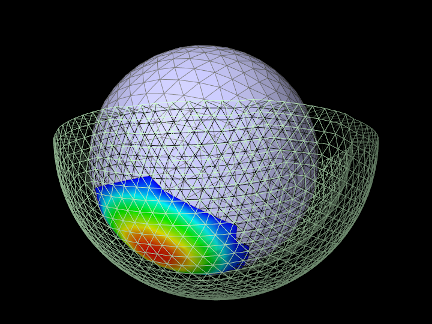
\includegraphics[]{../modelguide/images/ElasticFoundationContact}
\else
 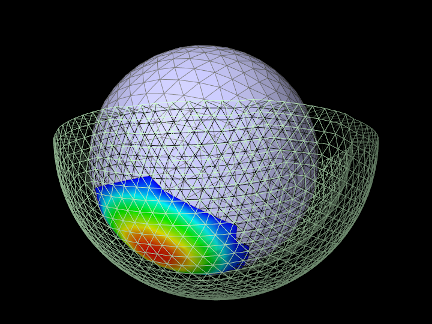
\includegraphics[width=3.75in]{../modelguide/images/ElasticFoundationContact}
\fi
\end{center}

Full details are given in the section ``Elastic foundation contact'',
in the (new) ``Contact and Collisions'' chapter of the
\href{http://www.artisynth.org/doc/pdf/modelguide.pdf}{Modeling
Guide}.

\subsubsection{New collision chapter in the Modeling Guide}

The \href{http://www.artisynth.org/doc/pdf/modelguide.pdf}{Modeling
Guide} has been revised to include a new ``Contact and Collision''
chapter specifically dedicated to explaining collision handling in
greater detail, with addtional code examples added to {\tt
artisynth.demos.tutorial}.

\subsubsection{Collision rendering property ``colorMapCollidable''
changed to ``renderingCollidable''}

The collision rendering property {\sf colorMapCollidable}, exported by both
\javaclass[artisynth.core.mechmodels]{CollisionManager} and
\javaclass[artisynth.core.mechmodels]{CollisionBehavior}, has been
changed to {\sf renderingCollidable}, and now controls the collidable
for which normals and contact forces are rendered, in addition to the
color map. The set/get accessors for {\sf colorMapCollidable} still
exist in deprecated form.

\subsubsection{Field components moved to artisynth.core.fields}

All application-level field components have been moved to the new
package {\tt artisynth.core.fields}, in order to reduce clutter in
other packages. Moved field components and their previous
packages are listed below:

\begin{tabular}{|ll|}
\hline
Component & Previous package\\
\hline
{\tt ScalarGridField} & {\tt artisynth.core.modelbase} \\
{\tt VectorGridField} & {\tt artisynth.core.modelbase} \\
{\tt ScalarNodalField} & {\tt artisynth.core.femmodels} \\
{\tt ScalarElementField} & {\tt artisynth.core.femmodels} \\
{\tt ScalarSubElemField} & {\tt artisynth.core.femmodels} \\
{\tt ScalarNodalField} & {\tt artisynth.core.femmodels} \\
{\tt ScalarElementField} & {\tt artisynth.core.femmodels} \\
{\tt ScalarSubElemField} & {\tt artisynth.core.femmodels} \\
{\tt VectorNodalField} & {\tt artisynth.core.femmodels} \\
{\tt Vector3dNodalField} & {\tt artisynth.core.femmodels} \\
{\tt VectorNdNodalField} & {\tt artisynth.core.femmodels} \\
{\tt MatrixNdNodalField} & {\tt artisynth.core.femmodels} \\
{\tt VectorElementField} & {\tt artisynth.core.femmodels} \\
{\tt Vector3dElementField} & {\tt artisynth.core.femmodels} \\
{\tt VectorNdElementField} & {\tt artisynth.core.femmodels} \\
{\tt MatrixNdElementField} & {\tt artisynth.core.femmodels} \\
{\tt VectorSubElemField} & {\tt artisynth.core.femmodels} \\
{\tt Vector3dSubElemField} & {\tt artisynth.core.femmodels} \\
{\tt VectorNdSubElemField} & {\tt artisynth.core.femmodels} \\
{\tt MatrixNdSubElemField} & {\tt artisynth.core.femmodels}
\end{tabular}

\subsubsection{API change for binding properties to fields}

Some component properties, primarly those related to FEM materials,
can be bound to a field such that their value varies over the field
domain. The API method for binding some property XXX to a field 
component of type {\tt T} has been changed from
%
\begin{lstlisting}[]
  setXXField (T field, boolean useRestPos)
\end{lstlisting}
%
to
%
\begin{lstlisting}[]
  setXXField (T field)
\end{lstlisting}
%
In other words, the second argument {\tt useRestPos} has been
removed. This argument applied only to the grid-based fields
\javaclass[artisynth.core.fields]{ScalarGridField} and
\javaclass[artisynth.core.fields]{VectorGridField}, and specified
whether or not rest positions should be used when determining values
for points within an FEM mesh. Instead, this behavior should now be
specified by setting the new {\sf useFemRestPosition} property within {\tt
ScalarGridField} or {\tt VectorGridField}.

\subsubsection{Field components for meshes}

Additional field components have been added to the package {\tt
artisynth.core.fields} to describe fields on meshes. At present, the
mesh types are restricted to triangular polygonal meshes. The field
component include:

\begin{description}

\item[ScalarVertexField]\mbox{}

Specifies scalar values at the mesh vertices. Values at points not
lying on a vertex are determined by first finding the nearest
(triangular) face to the point, and then interpolating from the vertex
values using the barycentric coordinates of the nearest point.

\item[VectorVertexField]\mbox{}

Specifies a vector value at the mesh vertices. Values at points not
lying on a vertex are determined by first finding the nearest
(triangular) face to the point, and then interpolating from the vertex
values using the barycentric coordinates of the nearest point.

\item[ScalarFaceField]\mbox{}

Specifies scalar values at the mesh faces. Values at points not lying
on a face are determined by finding the nearest (triangular) face to
the point, and then using the value for that face. Note that this
implies the field will generally be discontinuous.

\item[VectorFaceField]\mbox{}

Specifies vector values at the mesh faces. Values at points not lying
on a face are determined by finding the nearest (triangular) face to
the point, and then using the value for that face. Note that this
implies the field will generally be discontinuous. 

\end{description}

A primary use of mesh fields is to bind them to property values
associated with elastic foundation contact. In particular, the {\sf
YoungsModulus} and {\sf thickness} properties of
\javaclass[artisynth.core.materials]{LinearElasticContact} can be
bound to fields.

The vector fields can be defined for any
\javaclass[maspack.matrix]{VectorObject}.  Subclasses for specific
vector objects include:
%
\begin{lstlisting}[]
  Vector3dVertexField
  VectorNdVertexField
  Vector3dFaceField
  VectorNdFaceField
\end{lstlisting}
%

\section*{Apr 13, 2022}

ArtiSynth 3.7 has been released and is available on the website.  This
contains all current updates.

\subsubsection{Update to the Pardiso solver}

The Pardiso solver version has been updated to 2021.1.1, and contains
support for solves with multiple right hand sides. This is in
prepartion for the coming addition of implicit friction integration,
which will allow large Coulomb friction forces to be incorporated into
FEM models.

\section*{Mar 28, 2022}

\subsubsection{New OpenSim muscle materials}

New muscle and ligament materials based on OpenSim have been added to
{\tt core.materials}:

\begin{center}
\begin{tabular}{|ll|}
\hline
Material & Description \\
\hline
{\tt Thelen2003AxialMuscle} & rigid-tendon version of the OpenSim
Thelen2003Muscle\\
{\tt Blankevoort1991Ligament} & implements the OpenSim 
Blankevoort1991Ligament	\\
{\tt Millard2012AxialMuscle} & rigid-tendon version of the OpenSim 
Millard2012 muscle\\
\hline
\end{tabular}
\end{center}

\section*{Jan 28, 2022}

\subsubsection{Improved I/O for FEM models}

The ART file format for FEM models has been modified for greater
efficiency:

\begin{itemize}

\item Rest positions for {\tt FemNode3d} are no longer written to ART
files if they are the same as the current position.

\item Nodes for elements and {\tt FemMeshComp} attachments are now
stored and read by node number instead of component path name.
The previous format is still valid.

\item Meshes in {\tt FemMeshComp} are now written internally, using
the tag 'meshdata', if they are polygonal, not associated with a file,
and do not contain colors, textures, or explicit normals.

\end{itemize}

\subsubsection{Changes to {\tt maspack}}

\begin{itemize}

\item Added {\tt solvers.MurtyLCPSolver} to implement Murty's method
for LCPs and BLCPs, including block pivoting.

\item Added {\tt matrix.SparseCRSMatrix} as a simpler CRS-based sparse
matrix replacement for {\tt SparseMatrixCRS}.

\item Added methods to {\tt matrix.SparseBlockMatrix}: {\tt
removeRows()}, {\tt removeCols()}, {\tt addBlock(bi,bj,Matrix)}, {\tt
mul(MatrixNd,MatrixNd)}, {\tt mulLeft(MatrixNd,MatrixNd)},
and {\tt mulTransposeRight(MatrixNd,MatrixNd)}.

\item Added {\tt matrix.SparseBlockSignature} to represent the
structure of sparse block matrices.

\end{itemize}

\section*{Sep 16, 2021}

Some follow on updates from the Sep 12 update:

\subsubsection{Ability to set the UI look and feel}

A property called {\sf lookAndFeel} has been added to the layout
preferences, which allows one to set the UI look and feel, which is
based on Java Swing. See the ``Layout preferences'' section of the
\artisynthManual{uiguide}{User Interface Guide}.

\subsection*{More command line option changes}

Command line options related to the layout have been modified.  The
options {\tt -noTimeline} and {\tt timelineRight} have been removed,
and the following have been added:

\begin{center}
\begin{tabular}{|ll|}
\hline
Option & Description \\
\hline
{\tt -timelineVisible} & show the timeline at startup\\
{\tt -timelineHidden} & hide the timeline at startup\\
{\tt -timelineLocation <loc>} &
set the timeline location relative to the main frame\\
{\tt -jythonLocation <loc>} & 
set the Jython console location relative to the main frame\\
{\tt -lookAndFeel <laf>} & 
set the UI look and feel\\
\hline
\end{tabular}
\end{center}

\subsection*{Viewer property change}

The viewer property {\sf axisLengthRadiusRatio}, used when rendering
coordinate axes as solid arrows, has been replaced with {\sf
axisRadiusRatio}, with the value of the latter the inverse of the
former.

\section*{Sep 12, 2021}

A number of updates have been made, mainly with respect to the user
interface, allowing model and script menus to be customized, and other
settings and configuration information, including startup models, the
external classpath, and movie maker settings, to be stored in a
user-specific configuration folder. Other changes include a new
stop-all button that will halt both simulation and Jython scripts, and
new API support for removing model components in code.

\subsection*{New user configuration folder}

In order to separate user-specific settings from the ArtiSynth
installation, ArtiSynth now creates the configuration folder {\tt
ArtiSynthConfig} in the user's home folder, and uses this to store
various items such as preferences, model and script menus, the startup
model, model and script history, and the external classpath.

\subsection*{Revised model menu with editing}

The model menu, located under {\sf Models} in the main menu bar, has
been revised to include a number of new entries at the end:

\begin{center}
\iflatexml
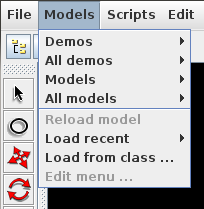
\includegraphics[]{images/modelMenu}
\else
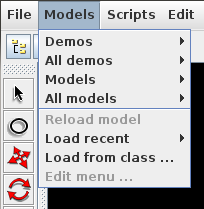
\includegraphics[width=1.75in]{images/modelMenu}
\fi
\end{center}

The {\sf ``Reload model''} and {\sf ``Load from class ...''}  entries
have been relocated from the {\sf File} menu, {\sf ``Load recent''}
has replaced {\sf ``Recent''}, and the entry {\sf ``Edit menu ...''}
opens a model menu editor that allows interactive editing of the
upper portion of the menu.

For details on menu editing, see ``Customizing the Model
and Script Menus'' in the \artisynthManual{uiguide}{User Interface
Guide}.

The XML files describing the model menu have also changed. The XML
format has been simplified, and the default menu file has been moved
from {\tt demoMenu.xml} in the ArtiSynth installation folder to {\tt
settings/modelMenu.xml} in the user configuration folder.

\subsection*{Revised script menu with editing}

The script menu, located under {\sf Scripts} in the main menu bar and
used to run Jython scripts, has been revised to include new entries
and make it feel-compatible with the model menu:

\begin{center}
\iflatexml
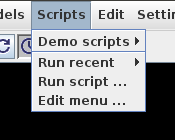
\includegraphics[]{images/scriptMenu}
\else
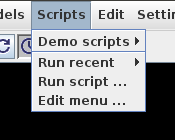
\includegraphics[width=1.5in]{images/scriptMenu}
\fi
\end{center}

{\sf ``Run script ...''} replaces {\sf ``Load script''} and opens a
dialog that allows the user to select a script, while {\sf ``Run
recent''} reruns recently run scripts.

The upper part of the script menu can be customized with an
arrangement of entries invoking specific scripts. This menu can be
customized in the same manner as the model menu by selecting {\sf
``Edit menu ...''} at the bottom. Script menu
information is contained in the file {\tt settings/scriptMenu.xml} in
the user configuration folder. The default menu supplies an entry
{\sf ``Demo scripts''} that expands to all scripts located in
%
\begin{verbatim}
  src/artisynth/demos/scripts
\end{verbatim}
%
relative to the ArtiSynth installation folder.

\subsection*{Revised settings menu}

The {\sf Settings} menu has been revised to allow additional control
over application properties related to the viewer, simulation control
and GUI interaction. These are collected into the menu items {\sf
``Viewers ...''}, {\sf ``Simulation ...''}, {\sf ``Interaction ...''},
and {\sf ``Mouse ...''}.

With respect to the previous entries, {\sf ``Background color''} and
{\sf ``Selection color''} are now controlled under {\sf ``Viewers
...''}; {\sf ``Mouse preferences ...''} is now {\sf ``Mouse ...''};
and {\sf ``Enabled articulated transforms''}, {\sf ``Visual display
rate''}, {\sf ``Real-time scaling''}, and {\sf ``Init draggers in
world coords''} are controlled by the properties {\sf
articulatedTransforms}, {\sf frameRate}, {\sf realTimeScaling}, and
{\sf initDraggersInWorld} located under {\sf ``Interaction ...''}.

See the ``Settings'' section in the \artisynthManual{uiguide}{User
Interface Guide}.

\subsection*{New preferences settings}

Many application properties, including those related to the viewer,
simulation control, GUI interaction, window layout, and movie making
can now be set permanently via the {\it preferences editor}, which can
be opened via {\sf Settings > Preferences ...}.

See the ``Preferences'' section in the
\artisynthManual{uiguide}{User Interface Guide}.

\subsection*{New stop-all button}

The play controls have been extended to include a new {\it stop-all}
button:
%
\begin{center}
\iflatexml

\includegraphics[]{../uiguide/images/playControls}
\else

\includegraphics[width=3in]{../uiguide/images/playControls}
\fi
\end{center}
%
Located at the right with a square icon, this buttons stops simulation
(in the same manner as the pause button), but also aborts any
currently running Jython command or script.

\subsection*{New support for deleting components in code}

A new static method has been added to
\javaclass[artisynth.core.modelbase]{ComponentUtils}:
%
\begin{lstlisting}[]
   ComponentUtils.deleteComponentsAndDependenices (comps);
\end{lstlisting}
%
where {\tt comps} is a list of model components. This can be used to
``prune'' components and their dependencies from existing models, with
a behavior that should be identical to selecting the components in the
GUI and then choosing {\sf Delete} from the context menu.

\subsection*{Simplified navigation panel visuals}

The navigation panel visuals have been simplified so that composite
component entries are now indicated with arrow icons (below, left),
instead of folders and lines (below, right):

\begin{center}
\begin{tabular}{cc}
\iflatexml
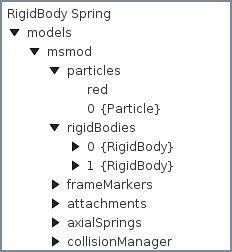
\includegraphics[]{images/navpanelNew}
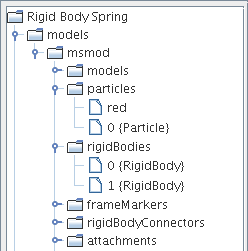
\includegraphics[]{images/navpanelOld}
\else
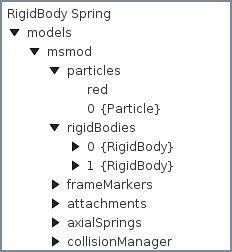
\includegraphics[width=2in]{images/navpanelNew}
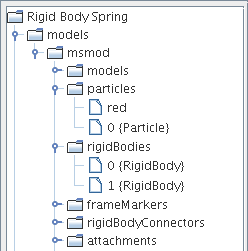
\includegraphics[width=2.1in]{images/navpanelOld}
\fi
\end{tabular}
\end{center}

\subsection*{Startup model now settable within ArtiSynth}

A startup model can now be set from within ArtiSynth to specify a
model (with optional {\tt build()} method arguments) to be loaded when
the application first starts. To do this, select {\sf Settings >
Startup model ...}. This capability replaces the need to specify such
models using the command line option {\tt -model <modelName>}
(although this command line option is still supported).

See ``Setting a startup model'' in the
\artisynthManual{uiguide}{User Interface Guide}.

\subsection*{External classpath now settable within ArtiSynth}

The external classpath, which contains class folders and JAR files for
models and packages located outside of {\tt artisynth\_core}, can now
be set from within ArtiSynth.  To do this, select {\sf Settings >
External classpath ...}, which opens an external classpath editor.
This capability replaces the need to edit the {\tt EXTCLASSPATH} file
by hand. The {\tt EXTCLASSPATH} file has also been moved to the user
configuration folder.

See ``Setting the external classpath'' in the
\artisynthManual{uiguide}{User Interface Guide}.

\subsection*{Libraries now updatable within ArtiSynth}

It is now possible to update the JAR files and native libraries from
within ArtiSynth, instead of calling
%
\begin{verbatim}
  bin/updateArtisynthLibs
\end{verbatim}
%
in the ArtiSynth installation folder.  Choose {\sf Update libraries}
from the {\sf File} menu.

\subsection*{Movie maker updates}

\begin{itemize}

\item The default folder for movie files is now {\tt
ArtiSynthConfig/movies} under the user's home folder.  This can also
be customized via {\sf Settings > Preferences > Movies > movie folder}.

\item A new {\sf Messages} tab has been added to the movie panel,
which displays the progress of move making commands along with any
error messages.

\item Customized command settings for the encoder options {\tt
FFMPEG}, {\tt MENCODER}, and {\tt AVCONV} can now be stored
permanently via {\sf Settings > Preferences > Movies} and selecting
{\sf Customize Method} for the selected method. In addition, there is
a new {\tt CUSTOM} method which can be set to {\it any} command-line
based movie making command available on the ArtiSynth host computer.

\item An explicit {\it stop time} can be set indicating when movie
recording should stop.

\end{itemize}

See the updated section ``Making Movies'' in the
\artisynthManual{uiguide}{User Interface Guide}.

\subsection*{Revised command line arguments}

The following command line options have been modified or removed:

\begin{center}
\begin{tabular}{|ll|}
\hline
Option & Change \\
\hline
{\tt -largeTimeline} & replaced with {\tt -timelineWidth <width>} and {
\tt -timelineHeight <height>} \\
{\tt -timelineZoom <level>} & replaced with {\tt -timelineRange <time>}\\
%%{\tt -home <ArtiSynthHomeDir>} & removed\\
{\tt -historyFile <file>} & removed\\
{\tt -updateLibs} & removed; choose {\sf File > Update libraries} 
from the main application menu instead\\
{\tt -demosMenu <file>} & renamed; use {\sf -modelMenu <file>} instead\\
{\tt -demosFile <file>} & renamed; use {\sf -demoFile <file>} instead\\
\hline
\end{tabular}
\end{center}

\subsection*{Enhanced help menu}

On systems where Java-browser integration is supported, the {\sf Help}
menu has been expanded to open browser windows to the modeling guide,
user interface guide, MATLAB interface manual, and Java API.

\subsection*{Jython documentation moved to the User Interface Guide}

Documentation for the Jython interface has been moved from the
``Interfacing ArtiSynth to MATLAB and Jython'' to the new section
``Jython Interaction and Scripting'' in the
\artisynthManual{uiguide}{User Interface Guide}, and the original
manual has been renamed to ``Interfacing ArtiSynth to MATLAB''.

\section*{Mar 5, 2021}

ArtiSynth 3.6 has been released and is available on the website.

\section*{Mar 4, 2021}

\subsection*{Pardiso updated to MKL 2021}

The Pardiso solver has been updated to MKL 2021.1. Users updating from
github should also run the command {\tt updateArtisynthLibs}.

\subsection*{New joint components}

A number of new joints have been added to ArtiSynth, including:

\begin{itemize}

\item
\javaclass[artisynth.core.mechmodels]{SliderJoint}:
1 DOF joint allowing translation along the
$z$ axis.

\item
\javaclass[artisynth.core.mechmodels]{CylindricalJoint}:
2 DOF joint allowing translation and
rotation along the $z$ axis.

\item
\javaclass[artisynth.core.mechmodels]{SkewedUniversalJoint}: 
2 DOF roll-pitch joint in which the roll-pitch axes may be at a
skewed angle relative to each other.

\item
\javaclass[artisynth.core.mechmodels]{PlanarJoint}:
3 DOF joint allowing translation and
rotation in the $x$-$y$ plane.

\item
\javaclass[artisynth.core.mechmodels]{PlanarTranslationJoint}: 
2 DOF joint allowing translation
in the $x$-$y$ plane.

\end{itemize}

In addition, the following joints have been added to replace {\tt
RevoluteJoint}, {\tt RollPitchJoint} and {\tt SphericalRpyJoint}:

\begin{itemize}

\item \javaclass[artisynth.core.mechmodels]{HingeJoint}: Identical to
{\tt RevoluteJoint}, except that its coordinate $\theta$ is oriented
{\it counter-clockwise} about the $z$ axis instead of {\it clockwise}.

\item
\javaclass[artisynth.core.mechmodels]{UniversalJoint}:
Identical to {\tt RollPitchJoint}, except
that its roll-pitch coordinates $\theta, \phi$ are computed with
respect to the rotation $\R_{CD}$ from frame C to D, instead of the
rotation $\R_{DC}$ from frame D to C.

\item \javaclass[artisynth.core.mechmodels]{SkewedUniversalJoint}:
Identical to {\tt SphericalRpyJoint}, except that its roll-pitch-yaw
coordinates $\theta, \phi, \psi$ are computed with respect to the
rotation $\R_{CD}$ from frame C to D, instead of the rotation
$\R_{DC}$ from frame D to C.

\end{itemize}

Rendering of the new joints is also controlled differently, with
the properties {\sf shaftLength}, {\sf shaftRadius}, and {\sf jointRadius}
used to control the size of the shaft and ball structures that are
drawn for visualization.

The old joints {\tt RevoluteJoint}, {\tt RollPitchJoint} and {\tt
SphericalRpyJoint} are still supported for legacy purposes.

Full details on the new joints, along with examples, are given in the
``Joint components'' section of the
\href{http://www.artisynth.org/doc/pdf/modelguide.pdf}
{Modeling Guide}.

\subsection*{Expanded joint documentation and custom joints}

The documentation in the
\href{http://www.artisynth.org/doc/pdf/modelguide.pdf} {Modeling
Guide} describing how joints and connectors are created, used and
implemented has been enhanced, with new sections describing
constraints, coordinates, constraint forces, and rendering.  In
addition, the joint implementation has been refactored to make it
easier to create custom joints, with full details given in the section
``Custom Joints'' in the chapter ``Mechanical Models II''.

\subsection*{API changes for joints and connectors}

Some small changes have been made to the methods for joints and
connectors:

\begin{itemize}

\item In joints and connectors which are subclasses of 
\javaclass[artisynth.core.mechmodels]{BodyConnector}, {\tt
numUnilateralConstraints()}, which returned the number of {\it
engaged} unilateral constraints, has been renamed to {\tt
numEnagedUnilateralConstraints()}. Similarly, in subclasses of
\javaclass[maspack.spatialmotion]{RigidBodyCoupling}, {\tt
numUnilaterals()} has been renamed to {\tt numEnagagedUnilaterals()}.

\item In joints and connectors which are subclasses of
\javaclass[artisynth.core.mechmodels]{BodyConnector}, {\tt
numUnilateralConstraints()} now returns the total number of unilateral
constraints, engaged or otherwise.  Similarly, in subclasses of
\javaclass[maspack.spatialmotion]{RigidBodyCoupling}, {\tt
maxUnilaterals()} has been renamed to {\tt numUnilaterals()}.

\item In subclasses of
\javaclass[artisynth.core.mechmodels]{BodyConnector}, the spatial
forces returned by the methods {\tt getBilateralForceInA()} are now
given in world coordinates. This was done to be consistent with {\tt
Frame} and {\tt RigidBody}, whose forces (returned by {\tt getForce()})
are also given in world coordinates.

\item In \javaclass[artisynth.core.mechmodels]{SphericalJoint},
rendering of the joint as a ball is now controlled by setting its {\sf
jointRadius} property, together with the {\sf faceColor} rendering
property, instead of the previous method of using point rendering
properties.

\end{itemize}

In addition to these changes, the penetration tolerance for unilateral
constraints which are {\it rotary} in nature is now controlled by the
{\sf rotaryLimitTol} property, exported by both {\tt MechModel} and
the joint classes.

New methods are also provided for determining the constraint forces
acting on a joint in different coordinate frames:
%
\begin{lstlisting}[]
   // returns constraint forces on joint frame C (in frame C coordinates):
   getBilteralForceInC()
   getUnilteralForceInC()

   // if bodyB is a frame, returns constraint forces on body B
   getBilteralForceInB()
   getUnilteralForceInB()
\end{lstlisting}
%

\subsection*{Reimplementation of skinning}

The class \javaclass[artisynth.core.femmodels]{SkinMeshBody}, which
implements skinning, has been rewritten to allow skinned meshes which
are connected to FEM models to behave properly under FEM rotation.

The {\tt SkinMeshBody} API has also been refactored to allow greater
flexibility in determining the connection weights between the mesh
vertices and the underlying rigid bodies and FEM models. Markers and
points can now be attached to a {\tt SkinMeshBody}, even in the
absence of a mesh, and this can be used as an simpler, more
approximate way to implement muscle wrapping behavior.

Full details on the updated skinning mechanism and how to use it are
given in the new chapter ``Skinning'' in the
\href{http://www.artisynth.org/doc/info/modelguide/modelguide.html}
{Modeling Guide}.

\subsection*{Improvements to large probe displays}

Large probe displays have been rewritten to provide higher quality
plotting, better interactive control, and the ability to export plots
to svg, postscript, and image files.

Full details on these changes are given in the ``Large displays''
section of the
\href{http://www.artisynth.org/doc/html/uiguide/uiguide.html} {User
Interface Guide}. To give a sense of the difference, the old display
looked like this,
%
\begin{center}
\iflatexml
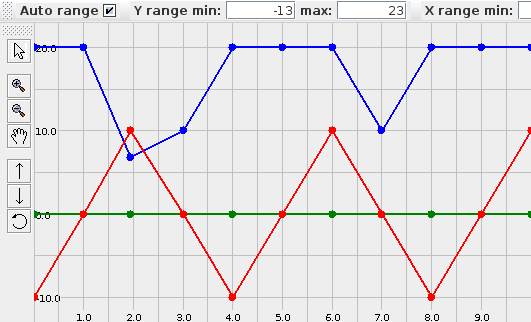
\includegraphics[]{images/largeProbeDisplayOld}
\else
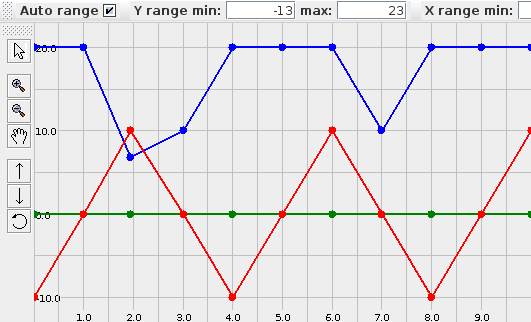
\includegraphics[width=0.66\textwidth]{images/largeProbeDisplayOld}
\fi
\end{center}
%
while the new display looks like this:
%
\begin{center}
\iflatexml
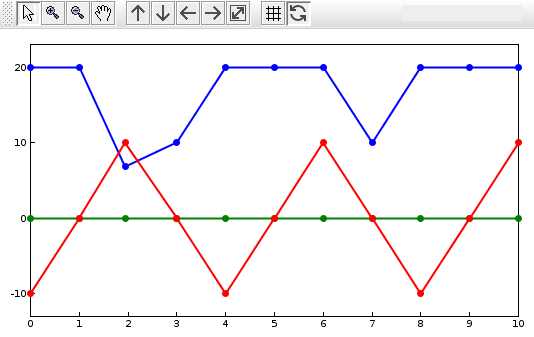
\includegraphics[]{images/largeProbeDisplayNew}
\else
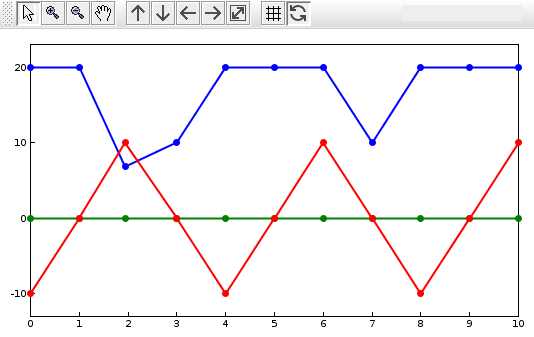
\includegraphics[width=0.66\textwidth]{images/largeProbeDisplayNew}
\fi
\end{center}
%

\subsection*{Solid arrow rendering of coordinate frames}

Frames and rigid bodies now have a new property called {\sf
axisDrawStyle}, that specifies how coordinate axes should be drawn.
Its type is the enumerated type {\tt Frame.AxisDrawStyle}, with the
possible values {\tt OFF}, {\tt LINE}, and {\tt ARROW}.  Setting it to
{\tt ARROW} will cause coordinate axes to be rendered as solid arrow,
as in this example:
\begin{center}
\iflatexml
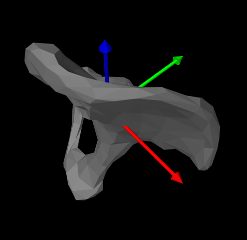
\includegraphics[]{images/hipBodyArrowAxes}
\else
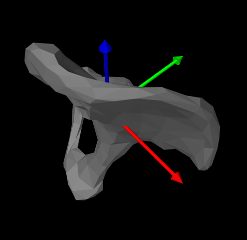
\includegraphics[width=0.4\textwidth]{images/hipBodyArrowAxes}
\fi
\end{center}

\subsection*{MAPStress and MAPStrain added to FEM surface rendering}

The enumerated type
\javaclass[artisynth.core.femmodels]{FemModel\$SurfaceRender}, which
controls the rendering of FEM surface meshes through an FEM model's
{\sf surfaceRendering} property, has been extended to include {\tt
MAPStress} and {\tt MAPStrain}, which render the surface as a color
map using the maximum absolute values of the principal stress and
strain components, respectively.

\section*{Apr 16, 2020}

\subsection*{Refactoring of the TrackingController}

The \javaclass[artisynth.core.inverse]{TrackingController}, which
provides ArtiSynth's inverse modeling capabilities, has been
refactored. This includes both internal code reorganization and
harmonization of the API.

\subsubsection*{Organization of cost and constraint terms}

The basic usage model for the tracking controller remains the same: an
application creates an instance of 
{\tt TrackingController}, adds it to the root model's controllers
using {\tt addController()}, and then populates it with various cost
and constraint terms for the quadratic program that is used to solve
for excitations.  However, the class organization for these terms has
been redesigned.

All terms now implement the interface
\javaclass[artisynth.core.inverse]{QPTerm}, with a base implementation
provided by \javaclass[artisynth.core.inverse]{QPTermBase}.  A {\tt
QPTerm} also uses
\javamethod[artisynth.core.inverse.QPTerm]{getType()} to specify its
type, which is defined by the enumerated type
\javaclass[artisynth.core.inverse]{QPTerm\$Type} and is either {\tt
COST} (cost term), {\tt INEQUALITY} (inequality constraint), or {\tt
EQUALITY} (equality constraint). These are implemented by
subinterfaces of {\tt QPTerm}: cost terms by
\javaclass[artisynth.core.inverse]{QPCostTerm} (with base
implementation \javaclass[artisynth.core.inverse]{QPCostTermBase})
and constraint terms by
\javaclass[artisynth.core.inverse]{QPConstraintTerm} (with base
implementation
\javaclass[artisynth.core.inverse]{QPConstraintTermBase}).  The
interface \javaclass[artisynth.core.inverse]{LeastSquaresTerm} (with
base implementation
\javaclass[artisynth.core.inverse]{LeastSquaresTermBase}) implements
{\it both} cost and constraint terms.

All cost and constraint terms are added to the controller as
subcomponents. Before performing each inverse computation, the
controller checks its subcomponents to find which terms to use.

\subsubsection*{Internal vs. external terms}

Cost and constraint terms are now either {\it internal} or {\it
external} to the controller. Internal terms include:
%
\begin{lstlisting}[]
  MotionTargetTerm     // cost/constraint term for point and frame tracking
  ForceTargetTerm      // cost/constraint term for joint force tracking
  ForceEffectorTerm    // cost/constraint term for force effector force tracking
  BoundsTerm           // inequality constraint term for excitation bounds
  L2RegularizationTerm // cost term for regularization excitation values
  DampingTerm          // cost term that inhibits how quickly excitations change
\end{lstlisting}
%
The {\tt MotionTargetTerm} and {\tt BoundsTerm} are always present in
the controller and can be accessed using
\javamethod[artisynth.core.inverse.TrackingController]{getMotionTargetTerm()}
and
\javamethod[artisynth.core.inverse.TrackingController]{getBoundsTerm()}.
Other internal terms can be added, removed or queried using {\it add},
{\it get} and {\it remove} methods. For example, for the 
{\tt ForceTargetTerm}, these methods are 
\javamethod[artisynth.core.inverse.TrackingController]{addForceTargetTerm()},
\javamethod[artisynth.core.inverse.TrackingController]{getForceTargetTerm()},
and
\javamethod[artisynth.core.inverse.TrackingController]{removeForceTargetTerm()}.

External terms include
\begin{lstlisting}[]
  NonuniformBoundsTerm // set explicit nonuniform excitation bounds
  ProportionalTerm     // cost term proportional to the sum of the excitations
\end{lstlisting}
%
as well as any custom terms implemented by an application. External
terms can be added added, removed and queried using
%
\begin{lstlisting}[]
  addCostTerm (term)
  removeCostTerm (term)
  getCostTerms()

  addConstraintTerm (term)
  removeConstraintTerm (term)
  getEqualityConstraints()
  getInequalityConstraints()
\end{lstlisting}
%

\begin{sideblock}
The previous methods {\tt addInequalityTerm} and {\tt
addEqualityTerm} have been replaced by {\tt addConstraintTerm}.
\end{sideblock}

\begin{sideblock}
The {\tt add} and {\tt remove} methods for external
terms should {\it not} be used for the internal terms. While it is
possible to create an instance of an internal term, such as {\tt
MotionTargetTerm}, and add it to the controller using {\tt
addCostTerm(term)}, this will simply add an {\it additional} motion
term to the controller that is separate from the internal one.
\end{sideblock}

\subsubsection*{Excitation components now stored using ExciterComp}

The excitation components used by the controller were previously
stored in a subcomponent list called {\tt "exciters"}. This was
actually incorrect since ArtiSynth components can not belong to more
than one list at a time.  In the revised implementation, {\tt
"exciters"} is now a list of {\tt ExcitationComp} objects, each of
which contains a reference to an excitation component along with an
associated weight. This means that excitation weights can now be set
interactively by changing the {\sf weight} property in each {\tt
ExcitationComp}.

\subsubsection*{Some term properties moved to the controller}

The following properties, which were previously present in some
individual cost and constraint terms, have now been moved to the
controller itself and should be set and queried there:
%
\begin{verbatim}
  useTimestepScaling
  useTrapezoidalSolver
  normalizeH 
  useKKTFactorAndSolve
\end{verbatim}
%

\subsubsection*{Target and source components now stored 
within their cost terms}

The previous version of the tracking controller contained the
following subcomponents, listing various target and source components
for the MotionTargetTerm and ForceTargetTerm:
%
\begin{lstlisting}[]
  exciters               // excitation components
  targetPoints           // target (reference) points for the MotionTargetTerm
  sourcePoints           // source (tracking) points for the MotionTargetTerm
  targetFrames           // target (reference) frames for the MotionTargetTerm
  sourceFrames           // source (tracking) frames for the MotionTargetTerm
  targetForces           // target (reference) forces for the ForceTargetTerm
\end{lstlisting}
%
In the refactored controller, the force and motion target terms have
been reimplemented as composite components, each maintaining lists of
their target and source components. Since (as indicated above) all
cost and constraint terms are now stored as controller subcomponents,
the resulting component hierarchy now looks like this:
%
\begin{lstlisting}[]
  exciters
  motionTerm
    targetPoints         // target (reference) points
    sourcePoints         // source (tracking) points 
    targetFrames         // source (tracking) frames 
    sourceFrames         // target (reference) frames
  boundsTerm
  L2RegularizationTerm
  forceTerm
    targetForces         // target (reference) forces
\end{lstlisting}
%

\subsubsection*{ForceMinimizationTerm renamed to ForceEffectorTerm}

The {\tt ForceMinimizationTerm} class has been renamed to
\javaclass[artisynth.core.inverse]{ForceEffectorTerm}, since it now
permits the forces produced by certain force effectors (those which
implement \javaclass[artisynth.core.mechmodels]{ForceTargetComponent}) to
be set to a particular target force. Setting that target force to zero
(which is the default value) will minimize the force. Likewise, the
{\tt ForceMinimizationTarget} class, which was used to describe each
force effector controlled by the {\tt ForceEffectorTerm}, has been
renamed to \javaclass[artisynth.core.inverse]{ForceEffectorTarget}.

\subsubsection*{``Enabled'' property replaced with ``active''}

The property {\sf enabled}, which was used to enable or disable the
controller, and was controlled using {\tt setEnabled(enable)} and {\tt
getEnabled()}, has been replaced by the property {\sf active}, which
is controlled using {\tt setActive(enable)} and {\tt getActive()} (and
already existed in the controller's base class).

\subsubsection*{Different names for probes created by InverseManager}

The names and file names of the probes created by the {\tt
InverseManager} have been changed to be more consistent. This affects
any of the probes created by the following methods:
%
\begin{lstlisting}[]
  // InverseManager methods (static):
  InverseManager.addProbes (rootModel, controller, duration, interval)
  InverseManager.resetProbes (rootModel, controller duration, interval)

  // TrackingController methods:
  createProbes (rootModel)
  createProbes (rootModel, duration, interval)
  createProbesAndPanel (rootModel)
  createProbesAndPanel (rootModel, duration, interval)
\end{lstlisting}
%
Probes created by the {\tt InverseManager} are now identified by an
enumerated type,
\javaclass[artisynth.core.inverse]{InverseManager\$ProbeID}, as
described in the next section. The old and new names associated with
these probes are:
%
\begin{center}
\begin{tabular}{|lll|}
\hline
Probe & old name & new name \\
\hline
{\tt TARGET\_POSITIONS} & {\tt "target positions"} & {\it unchanged} \\
{\tt TARGET\_FORCES} & {\tt "target forces"} & {\it unchanged} \\
{\tt INPUT\_EXCITATIONS} & {\tt "input excitations"} & {\it unchanged} \\
{\tt TRACKED\_POSITIONS} & {\tt "target positions"} & {\tt "tracked positions"} \\
{\tt SOURCE\_POSITIONS} & {\tt "model positions"} & {\tt "source positions"} \\
{\tt COMPUTED\_EXCITATIONS} & {\tt "input excitations"} & {\it unchanged} \\
\hline
\end{tabular}
\end{center}
%
while the old and new file names are:
%
\begin{center}
\begin{tabular}{|lll|}
\hline
Probe & old name & new name \\
\hline
{\tt TARGET\_POSITIONS} & {\tt "ref\_targetPos\_input.txt"} & {\tt "target\_positions.txt} \\
{\tt TARGET\_FORCES} & {\tt "ref\_targetForce\_input.txt"} & {\tt "target\_forces.txt"} \\
{\tt INPUT\_EXCITATIONS} & {\tt "excitations\_input.txt"} & {\tt "input\_excitations.txt"} \\
{\tt TRACKED\_POSITIONS} & {\tt "ref\_target\_positions.txt"} & {\tt "tracked\_positions.txt"} \\
{\tt SOURCE\_POSITIONS} & {\tt "model\_target\_positions.txt"} & {\tt "source\_positions.txt"} \\
{\tt COMPUTED\_EXCITATIONS} & {\tt "excitations.txt"} & {\tt "computed\_excitations.txt"} \\
\hline
\end{tabular}
\end{center}
%

\begin{sideblock}
To revert to the previous naming conventions, applications can set the
static attribute {\tt InverseManager.useLegacyNames} to {\tt true}.
\end{sideblock}

\subsubsection*{Different default probe update interval}

The {\tt TrackingController} property {\sf probeInterval}, which
controls the update interval for the output probes created by
%
\begin{lstlisting}[]
  createProbes (rootModel);
  createProbesAndPanel (rootModel);
\end{lstlisting}
%
now has a default value of {\tt -1}, which causes the output probes to
be updated at the current simulation rate. The previous default value
was {\tt 0.01}. To revert to this value, one can set the static
attribute {\tt TrackingController.DEFAULT\_PROBE\_INTERVAL} to {\tt
0.01}.

\subsubsection*{Refactoring of the InverseManager}

The InverseManager, which is a utility class for creating probes and a
control panel for use with the tracking controller, has been
refactored so that all its methods are now static and take a root
model as one of their arguments. The primary methods are:
%
\begin{lstlisting}[]
  // create probes and add them to the root model:
  addProbes (root, controller, duration, interval) 

  // clear all probes, and then call addProbes():
  resetProbes (root, controller, duration, interval)

  // create a control panel for the tracking controller
  addInversePanel (root, controller)
\end{lstlisting}
%
As before, the {\tt addProbes()} method creates three input probes and
three output probes. Each probes starts at time 0 and has a stop time
indicated by {\tt duration}, while the output probes have an update
interval given by {\tt interval}. The probes themselves are now
identified by the enumerated type
\javaclass[artisynth.core.inverse]{InverseManager\$ProbeID}.
The input probes are:
%
\begin{lstlisting}[]
 TARGET_POSITIONS     // desired trajectory for all motion targets
 TARGET_FORCES        // desired trajectory for all constraint force targets
 INPUT_EXCITATIONS    // input excitations to used for forward simulation
\end{lstlisting}
%
Once created, these can be located and managed within the root model using
the {\tt InverseManager} methods
%
\begin{lstlisting}[]
  findInputProbe (root, probeId)
  setInputProbeData (root, probeId, data, timeStep)
\end{lstlisting}
%
The output probes are:
%
\begin{lstlisting}[]
 TARGET_POSITIONS     // updated observed trajectory for all motion targets
 SOURCE_POSITIONS     // actual trajectory for all motion targets
 COMPUTED_EXCITATIONS // excitations computed by the inverse solver
\end{lstlisting}
%
and can be located within the root model using the
method
%
\begin{lstlisting}[]
  findOutputProbe (root, probeId)
\end{lstlisting}
%

Also as before, the {\tt createPanel()} method creates a control panel
for viewing and adjusting controller properties, and adds it to the
root model. After, the panel can be located within the root model
using the method {\tt findInversePanel(root)}.

Similar to before, the {\tt TrackingController} supplies the
convenience methods
%
\begin{lstlisting}[]
  createProbes (rootModel)
  createProbes (rootModel, duration, interval)
  createProbesAndPanel (rootModel)
  createProbesAndPanel (rootModel, duration, interval)
\end{lstlisting}
%
which create probes and panels, with {\tt createProbes(rootModel)} and
{\tt createProbesAndPanel(rootModel)} using the controller's {\sf
probeDuration} and {\sf probeInterval} properties to supply the {\tt
duration} and {\tt interval} information.

More details on the \javaclass[artisynth.core.inverse]{InverseManager}
can be found in its API documentation.

\section*{Jan 22, 2020}

\subsection*{Export for numeric probes}

It is now possible to export numeric probe data as either a {\tt .csv}
or {\tt .txt} files. To do this, select the probe (in either the
navigation panel or the timeline), and choose {\sf Export} or {\sf
Export as ...} from the context menu.

\subsection*{Resetting the initial state}

The RootModel now contains the method {\tt resetInitialState()}, which
causes the initial state (i.e., the state at time 0) to be reset to
the current state.

This can also be called interactively using the new {\sf reset state}
button 
\iflatexml

\includegraphics[]{../uiguide/images/resetState} 
\else

\includegraphics[width=0.2in]{../uiguide/images/resetState} 
\fi
located at the top left.

\subsection*{Disabling realtime simulation}

By default, when running with graphics enabled, the simulation tries
to run in real time, with the simulation slowed down (if necessary) so
it does not proceed faster then real time. This can now be disabled,
using the {\tt Main} method {\tt setRealTimeAdvancement(enable)}, so
that the simulation runs as fast as possible. Note that real-time
advancement is disabled by default when running in batch mode, which
is why batch simulations sometimes run faster.

Real-time advancement can also be controlled with the new {\sf
real-time enable} button
\iflatexml

\includegraphics[]{../uiguide/images/realtimeEnable} 
\else

\includegraphics[width=0.2in]{../uiguide/images/realtimeEnable} 
\fi
located at the top left.

\subsection*{Full play controls added to the main viewer}

The play controls in the main viewer have been extended to include the
skip-back and skip-forward buttons that advance the model across
waypoints.

\subsection*{Embedded FEM support}

A new set of utility methods has been added for creating embedded FEM
models, and in particular voxelized embedding FEMs. The utilities were
originally created by Antonio S\'{a}nchez and have now been added to the
package {\tt core.femmodels}, with the main class being {\tt
EmbeddedFem}. Two of its principal methods are:
%
\begin{lstlisting}[]
   static FemModel3d createBoundingFem (
      FemModel3d fem, PolygonalMesh mesh, RigidTransform3d trans, 
      int minRes, double maxElemWidth, double margin)

   static FemModel3d createVoxelizedFem (
      FemModel3d fem, PolygonalMesh mesh, RigidTransform3d trans, 
      int minRes, double maxElemWidth, double margin)
\end{lstlisting}
%

\section*{Sep 19, 2019}

\subsection*{Enhancements to saving models}

When saving a model to a file using the {\sf Save model as ...} menu
item, users can now choose the following options:

\begin{description}

\item[Save waypoint data:] \mbox{}

Causes the state data for any valid waypoints to be saved in addition
to the waypoint locations.  This is optional because a large number of
waypoints may significantly increase the file size for models with
large state sizes.

\item[Core components only:] \mbox{}

Save only those components which are present in the main {\tt
artisynth\_core} package. Any non-core components, and any other
components which have a hard dependency on them, will not be written,
and the user will be advised of this via a message dialog.  The root
model is saved as a pure instance of {\tt RootModel}, instead of the
application-specific class that was used to build it. This means that
any properties or class overrides specific to the application root
model class will not be present in the saved model. The advantage to
storing a model using only core components is that it can be loaded by
any other user running that same ArtiSynth version, without needing
access to any application-specific classes.

\end{description}

\subsection*{Enhancements to waypoint data}

Waypoint data files (such as those written using the menu items {\sf
Save waypoints as ...}  and {\sf Save waypoints}) now contain
annotations so that when they are later loaded into a model, checks
are performed to help ensure that the state is consistent with that
model.

\subsection*{Easier reading and writing of meshes}

It is now possible to construct, read, or write any of the mesh
components (\javaclass[maspack.geometry]{PolygonalMesh},
\javaclass[maspack.geometry]{PolylineMesh},
\javaclass[maspack.geometry]{PointMesh}) by simply specifying a file
and then have the file format inferred directly from the file suffix.
The currently supported file formats, and their applicability to the
different mesh types, are given in the table below:

\begin{center}
\begin{tabular}{|ll|ccc|}
\hline
Suffix & Format & {\tt PolygonalMesh} & {\tt PolylineMesh} & {\tt PointMesh} \\
\hline
.obj & Alias Wavefront &X&X&X\\
.ply & Polygon file format &X&&X\\
.stl & STereoLithography &X&&\\
.gts & GNU triangulated surface &X&&\\
.off & Object file format &X&&\\
.vtk & VTK ascii format &X&&\\
.vtp & VTK XML format &X&X&\\
\hline
\end{tabular}
\end{center}

The new constructors are
%
\begin{lstlisting}[]
   PolygonalMesh (String fileName) throws IOException
   PolygonalMesh (File file) throws IOException

   PolylineMesh (String fileName) throws IOException
   PolylineMesh (File file) throws IOException

   PointMesh (String fileName) throws IOException
   PointMesh (File file) throws IOException
\end{lstlisting}
%
and the new read/write methods are:
\begin{lstlisting}[]
   read (File file) throws IOException
   write (File file) throws IOException

   read (File file, boolean zeroIndexed) throws IOException
   write (File file, String fmtStr, boolean zeroIndexed) throws IOException
\end{lstlisting}
%
For the latter methods, the argument {\tt zeroIndexed} specifies
zero-based vertex indexing (in the case of Alias Wavefront {\tt .obj}
files), while {\tt fmtStr} is a C-style format string specifying the
precision and style with which the vertex coordinates should be
written. (In the former methods, zero-based indexing is false and
vertices are written using full precision.)

\begin{sideblock}
Note: the method
\begin{verbatim}
   read (File file, String fmtStr)
\end{verbatim}
which was specific to {\tt PolygonalMesh}, has been removed.
In its place, one can use
\begin{verbatim}
   read (File file, String fmtStr, boolean zeroIndexed)
\end{verbatim}
with {\tt zeroIndexed} set to false.
\end{sideblock}

\subsection*{New scripting commands}

New commands have been added to the Matlab and Jython scripting
interfaces for saving and loading models and waypoints,
%
\begin{lstlisting}[]
   saveModelFile (filename)
   saveModelFile (filename, saveWayPoints, coreCompsOnly)

   saveWayPoints (filename)
   loadWayPoints (filename)
\end{lstlisting}
%
where {\tt saveWayPoints} specifies whether to save waypoint data and
{\tt coreCompsOnly} specifies whether to save only core components, as
described above.

\subsection*{ClassAliases moved to maspack.util}

The ClassAliases package, which maps class names onto (shorter)
aliases, and now also provides support for checking to see if a class
is contained in {\tt artisynth\_core}, has been moved to {\tt
maspack.util}.

\section*{Jul 21, 2019}

\subsection*{Field components added}

Field components have been added to allow the interpolation of both
scalar and vector quantities over regular and FEM-based grids.  Once
created, a field can be ``bound'' to properties of various FEM
materials, allowing the values of these properties to vary over the
FEM domain. For example, the stiffness parameters of an FEM material
may vary at different points within the volumetric mesh.

Full documentation on creating fields and binding them to materials is
given in the new section ``Fields'', in the ``Finite Element Models''
chapter of the the
\href{http://www.artisynth.org/doc/info/modelguide/modelguide.html}
{Modeling Guide}.

\subsection*{MaterialBundles added to FemModel3d}

FemModel3d now supports the ability to add ``material bundles'', which
allow supplemental materials to be added to the elements of an FEM
model.  A material bundle can be specified for either all elements or
selected elements within the model. 

Material bundles are implemented using the class
\javaclass[artisynth.core.femmodels]{MaterialBundle}, and are
analogous to {\tt MuscleBundle}, except that they can be used for any
type of FEM material and don't specify excitation or excitation
directions.  It is possible to use a {\tt MaterialBundle} to implement a
muscle behavior, by specifying a {\tt MuscleMaterial} whose {\sf
excitation} and {\sf restDir} properties are set directly by the
application (with the latter possibly attached to a {\tt Vector3d} field).

Full documentation is given in the new section ``Varying and
augmenting materials'', in the ``Finite Element Models'' chapter of
the the
\href{http://www.artisynth.org/doc/info/modelguide/modelguide.html}
{Modeling Guide}.

\subsection*{Refactoring of FEM materials}

FEM materials have been refactored in several ways:

\begin{itemize}

\item The {\tt computeStress()} and {\tt computeTangent()} methods are
now consolidated into a single method \\ {\tt
computeStressAndTangent()} (in which the argument to return the
tangent matrix is optional). The main reason for this is efficiency:
tangent calculations often require some of the same calculations
required for stress, and so computing these quantities in the same
method avoids repeated computation.

\item The property {\sf viscoBehavior} has been removed from {\tt
FemMaterial}. Instead, viscoelasticity is now effected by creating an
instance of
\javaclass[artisynth.core.materials]{ViscoelasticMaterial}, which
takes both a base material and a viscoelastic behavior.

\item FEM materials can now maintain their own
custom state. This is done via the interface 
\javaclass[artisynth.core.materials]{HasMaterialState},
which supplies the methods
%
\begin{lstlisting}[]
  // material currently has state
  boolean hasState(); 

  // creates an object for storing the state
  MaterialStateObject createStateObject();

  // advances the state from time t0 to t1
  advanceState (MaterialStateObject state, double t0, double t1);
\end{lstlisting}
%
For materials which have state, the system creates state instances
which are stored at each element integration point and supplied as an
additional argument to the {\tt computeStressAndTangent()} method.

\item A new FEM material,
\javaclass[artisynth.core.materials]{ScaledFemMaterial}, has been added
which takes a base material and a scaling factor. The latter can then be
attached to a scalar field to ``scale'' the effect of the material
over an entire FEM. The old way of doing this, which involved a
scaling factor in the integration data (class {\tt
IntegrationData3d}), has been removed.

\end{itemize}

\subsection*{MuscleBundle can now accept shell elements}

\javaclass[artisynth.core.femmodels]{MuscleBundle} and
\javaclass[artisynth.core.femmodels]{MuscleElementDesc} have been
extended to allow shell as well as volumetric elements. This means
that elements for these objects are now referenced by {\tt
FemElement3dBase} instead of {\tt FemElement3d}.

\subsection*{AuxiliaryMaterials now deprecated}

With the addition of {\tt MaterialBundles}, the existing means for
added ``extra'' materials to an FEM, using \\
{\tt AuxiliaryMaterial}, is
now deprecated. {\tt AuxiliaryMaterials} are still used ``under the
hood'' to implement {\tt MuscleBundles}, but it is expected that they
will eventually be removed.

An undocumented feature known as {\tt AuxMaterialBundle} currently
exists within ArtiSynth, which allows \\ 
{\tt AuxiliaryMaterials} to be
added to an FEM model in a manner analogous to {\tt MaterialBundle}.
To accommodate {\tt MaterialBundle}, the methods for adding, removing
and accessing {\tt AuxMaterialBundles} have been renamed as follows:

\begin{tabular}{ll}
\hline
Old method & New method \\
\hline
{\tt getMaterialBundles()} & {\tt getAuxMaterialBundles()} \\
{\tt addMaterialBundle(bundle)} & {\tt addAuxMaterialBundle(bundle)} \\
{\tt removeMaterialBundle(bundle)} & {\tt removeAuxMaterialBundle(bundle)} \\
{\tt clearMaterialBundles()} & {\tt clearAuxMaterialBundles()}\\
\hline
\end{tabular}

\subsection*{MuscleElementDesc not longer extends ExcitationComponent}

To quickly review: A
\javaclass[artisynth.core.femmodels]{MuscleBundle} is the basic
grouping of elements within an
\javaclass[artisynth.core.femmodels]{FemMuscleModel} that share a
single excitation value.  Each element within a {\tt MuscleBundle} is
described by a single
\javaclass[artisynth.core.femmodels]{MuscleElementDesc}. Removing the
\javaclass[artisynth.core.mechmodels]{ExcitationComponent} interface
from {\tt MuscleElementDesc} means that it is no longer be possible to
control the excitation for one or more {\tt MuscleElementDescs} {\it
separately} from the excitation of the {\tt MuscleBundle}. In other
words, a {\tt MuscleBundle} now represents the smallest possible
grouping of FEM elements for which you can provide a single
excitation.

Note that as before, one is still able to combine the excitations of
several MuscleBundles using MuscleExciter components.

\subsection*{Other changes}

\begin{itemize}

\item Excitation component has been simplified by removing the methods
%
\begin{lstlisting}[]
  void addExcitationSource(ExcitationComponent ex)

  double getDefaultActivationWeight()
\end{lstlisting}
%

\item In the {\tt maspack.properties} package, added {\tt
setAllowedTypes()} to {\tt PropertyDesc}, to specify which subclasses
of {\tt getValueClass()} may be used for creating instances of a
property within a {\tt CompositePropertyPanel}.

\item In {\tt maspack.widgets}, modified {\tt CompositePropertyPanel}
to use reflection to look for the method \\ {\tt
initializePropertyValues()} in the declaration of a {\tt
CompositeProperty}, and use this to help initialize the subproperties
of a {\tt CompositeProperty} based on the value of a previous
object with the same base class.

\item Added the methods {\tt getMaxAbsPrincipalStress()} and {\tt
getMaxAbsPrincipalStrain()} to
\javaclass[artisynth.core.femmodels]{FemNode3d}.

\end{itemize}

\section*{May 6, 2019}

\subsection*{Enhanced rigid body inertia computation}

The method by which inertia is automatically computed for a rigid body
based on the geometry of its mesh components (when its {\sf
inertiaMethod} is {\tt MASS} or {\tt DENSITY}) has been improved.
Mesh components now have a property {\sf massDistribution} which
determines how the mesh's inertia contribution is determined for a
given mass.  {\tt VOLUME}, {\tt AREA}, {\tt LENGTH}, and {\tt POINT}
indicate, respectively, that the mass is distributed evenly over the
mesh's volume, area (faces), length (edges), or points. The default
value is determined by the mesh type: {\tt VOLUME} for a closed {\tt
PolygonalMesh}, {\tt AREA} for an open {\tt PolygonalMesh}, {\tt
LENGTH} for a {\tt PolylineMesh}, and {\tt POINT} for a {\tt
PointMesh}. Applications can specify an alternate value providing the
mesh has the features to support it. Specifying {\tt DEFAULT} will
restore the default value.should be determined.

Full details are given in the section ``Multiple meshes'',
located under ``Rigid bodies'', in the
\href{http://www.artisynth.org/doc/info/modelguide/modelguide.html}
{Modeling Guide}.

\subsection*{Saving models in mid-simulation}

It is now possible to save a model to a file in mid-simulation.
Previously, it was assumed that the simulation ``time'' was 0.  Now,
however, you can simulate to some time $t$, and then save the model
(using {\sf File > Save model as ...}). Loading the resulting file
(using {\sf File > Load model ...}) will restore the model to the
simulation time $t$.

If the model contains valid waypoints, the state of these waypoints is
now also saved and restored. One caution is that if there are many
waypoints and the model state is large, the resulting save file may
also be quite large.

\subsection*{Forces and nodal stress/strains now saved as
state}

Forces and nodal stress/strain values are now saved as state within
waypoints.  This ensures that when a model is reset to a given
waypoint at time $t$, forces and stress/strains will be reset to the
same values they had when the simulation originally reached $t$.

\subsection*{Improvement and simplification of the state mechanism}

The interface {\tt HasAuxState}, used to indicate components which
store state, has been renamed to {\tt HasNumericState} and moved to
{\tt artisynth.core.modelbase}. It has also been simplified, with the
methods {\tt skipAuxState()} and {\tt getInitialState()} removed and
{\tt getAuxState()}, {\tt setAuxState()}, and {\tt advanceAuxState()}
renamed to {\tt getState()}, {\tt setState()} and {\tt
advanceState()}.

Numerous internal changes have been made to the mechanism by which
model state is saved and restored, both from waypoints and from model
files, largely with the goal of ensuring exact repeatability of results
when simulation resumes from a previously stored state.

\subsection*{Menu command for saving and loading waypoints}

A new set of menu commands have been added for saving and loading
waypoints. These are accessed from the {\sf File} menu and include:

\begin{description}

\item[Load wayPoints ...]\mbox{}

Loads a set of waypoints from a specified file. As before, loading
waypoints are superimposed on top of any existing waypoints.

\item[Save wayPoints as ...]\mbox{}

Saves the current set of waypoints to a specified file.

\item[Save wayPoints]\mbox{}

Saves the current set of waypoints to a previously specified file.

\end{description}

Previously, saving and loading waypoints had to be performed from the
timeline. The save file now also includes information for all
waypoints, with or without state, along with information identifying
breakpoints.

As before, the waypoint data file is binary, since this typically
requires half the file size and improves file I/O times by as much as
tenfold.

\subsection*{Changes to nodal stress/strain computation and 
contact rendering}

Stress or strain computation can now be explicitly enabled for
individual FEM nodes via the {\sf computeStress} and {\sf
computeStrain} properties of
\javaclass[artisynth.core.femmodels]{FemNode3d}.  Otherwise, when
needed for {\tt Stress} or {\tt Strain} rendering of an FEM mesh,
nodal computation of stress/strain is now optimized to require
computation of stress/strain values only for those nodes associated
with the mesh.

A new property {\sf colorMapInterpolation} has been added to
\javaclass[artisynth.core.mechmodels]{CollisionManager} and
\javaclass[artisynth.core.mechmodels]{CollisionBehavior}
to control color interpolation when a penetration depth or
contact pressure map is requested via the {\sf drawColorMap} property.
The default interpolation is HSV.

\subsection*{Constraint impulses now stored as forces}

Bilateral and unilateral constraint impulses are now converted to
forces when they are stored in the model. This means that it is no
longer necessary to convert impulses to forces by dividing by the
simulation time step. In particular:

\begin{itemize}

\item The methods {\tt setBilateralImpulses(lam,h,idx)} and {\tt
setUnilateralImpulses(the,h,idx)} (in {\tt MechSystem} and {\tt
Constrainer}) have been changed to {\tt setBilateralForces(lam,s,idx)}
and {\tt setUnilateralForces(the,s,idx)}. Within each of these, the
forces should be computed from {\tt s*lam} and {\tt s*the}.

\item The methods {\tt getBilateralImpulses(lam,idx)} and {\tt
getUnilateralImpulses(the,idx)} have been changed to {\tt
getBilateralForces(lam,idx)} and {\tt getUnilateralForces(the,idx)}.

\item Related '{\tt Impulse}' methods have been renamed to '{\tt
Force}'.

\item {\tt CollisionResponse.getContactImpulses()} has been changed to
{\tt getContactForces()}.

\item The last argument for {\tt
ContactForceBehavior.computeResponse()} has been changed from {\tt
region} (giving the contact's penetration region) to {\tt contactArea}
(which gives the estimated average area associated with the contact).

\end{itemize}

\section*{Feb 11, 2019}
%
\subsection*{Muscle wrapping added}

Muscle wrapping has now been officially added to ArtiSynth, with
documentation supplied by a new chapter called ``Muscle Wrapping'' in
the
\href{http://www.artisynth.org/doc/info/modelguide/modelguide.html}
{Modeling Guide}.  This documentation refers to a number of examples
that have been added to {\tt artisynth.demos.tutorials}.

\subsection*{RigidBody and RigidCompositeBody Merged}

It is now possible to add multiple meshes to a 
\javaclass[artisynth.core.mechmodels]{RigidBody},
subsuming the functionality previously offered by {\tt
RigidCompositeBody}, which is now deprecated.

Each rigid body mesh is stored in a mesh component, 
\javaclass[artisynth.core.mechmodels]{RigidMeshComp}, which is in turn
contained in a subcomponent list named {\tt meshes}. Meshes can be of
any type, including 
\javaclass[maspack.geometry]{PolygonalMesh},
\javaclass[maspack.geometry]{PolylineMesh} and
\javaclass[maspack.geometry]{PointMesh}.
The method 
\javamethod[\mech.RigidBody]{getSurfaceMesh()}
returns the first {\tt PolygonalMesh} in the list, and 
\javamethod[\mech.RigidBody]{getSurfaceMeshComp()}
returns its associated {\tt RigidMeshComp}.

Meshes can be added to a {\tt RigidBody} by creating a {\tt
RigidMeshComp} for them and then using methods such as
%
\begin{lstlisting}[]
  void addMeshComp (RigidMeshComp mcomp)
  boolean removeMeshComp (RigidMeshComp mcomp)
  int numMeshComps()
  void clearMeshComps()
\end{lstlisting}
%
They can also be added directly, using the methods
%
\begin{lstlisting}[]
  RigidMeshComp addMesh (MeshBase base)
  RigidMeshComp addMesh (MeshBase base, boolean hasMass, boolean isCollidable)
\end{lstlisting}
%
which allocate and return a {\tt RigidMeshComp}.  The latter method
also specifies {\tt hasMass}, which indicates if the mesh should
contribute to the body's inertia, and {\tt isCollidable}, which
indicates if it should contribute to the body's collision mesh.

\javaclass[artisynth.core.mechmodels]{RigidMeshComp} also contains new
properties, {\sf mass} and {\sf density}, that can directly control
how the mesh contributes to the rigid body's inertia when
its {\sf inertiaMethod} is {\tt MASS} or {\tt DENSITY}.

Full details are given in the new section ``Multiple meshes'',
located under ``Rigid bodies'', in the
\href{http://www.artisynth.org/doc/info/modelguide/modelguide.html}
{Modeling Guide}.

\subsection*{Distance grids stored in DistanceGridComp}

A new component, \javaclass[\mech]{DistanceGridComp}, has been added
for containing, controlling, and visualizing the distances grids
represented by \javaclass[\mgeo]{DistanceGrid}.
Full documentation is given in the new section
``Distance Grids and Components'' in the 
\href{http://www.artisynth.org/doc/info/modelguide/modelguide.html}
{Modeling Guide}.

In particular, the distance grid for a rigid body has been moved into
its own {\tt DistanceGridComp}, which is a subcomponent of the body
named {\tt "distanceGrid"}. One can obtain a reference to the grid
component via the method
%
\begin{lstlisting}[]
  DistanceGridComp getDistanceGridComp();
\end{lstlisting}
%

\subsection*{API changes involving RigidBody}

The wrapping code and the removal of {\tt RigidCompositeBody} have
engendered some API changes involving {\tt RigidBody}.

1) The following methods concerning surface meshes have been renamed. The
old methods have been retained but deprecated:

\begin{tabular}{ll}
\hline
Old method & New method \\
\hline
{\tt getMesh()} & {\tt getSurfaceMesh()} \\
{\tt setMesh(mesh)} & {\tt setSurfaceMesh(mesh)} \\
{\tt setMesh(mesh,fileName)} & {\tt setSurfaceMesh(mesh,fileName)}\\
{\tt setMesh(mesh,fileName,X)} & {\tt setSurfaceMesh(mesh,fileName,X)}\\
\hline
\end{tabular}

2) The field names for the enumerated type {\tt RigidBody.InertiaMethod}
have been capitalized, so that {\tt Density}, {\tt Mass}, and {\tt
Explicit} are now {\tt DENSITY}, {\tt MASS}, and {\tt EXPLICIT}.

3) The rigid body's distance grid has been moved into its own
component, which is a {\tt DistanceGridComp} that can be obtained via
{\tt getDistanceGridComp()}. The old {\tt RigidBody} properties for
controlling the distance grid have therefore been replaced by their
equivalent properties in the grid component:

\begin{tabular}{ll}
\hline
Old {\tt RigidBody} property & New {\tt DistanceGridComp} property \\
\hline
{\sf distanceGridRes} & {\sf resolution} \\
{\sf distanceGridMaxRes} & {\sf maxResolution} \\
{\sf distanceGridOBB} & {\sf fitWithOBB} \\
{\sf distanceSurfaceIso} & {\sf surfaceDistance} \\
{\sf renderDistanceGrid} & {\sf renderGrid} \\
{\sf distanceGridRenderRanges} & {\sf renderRanges} \\
\hline
\end{tabular}

In addition, the old {\tt RigidBody} property {\sf
renderDistanceSurface} has been replaced by the combination of the
{\tt DistanceGridComp} properties {\sf renderSurface} and {\sf
surfaceType}, along with the new {\tt RigidBody} property {\sf
gridSurfaceRendering}. The latter, if set {\tt true}, will cause the
grid's isosurface to be rendered instead of the rigid body mesh
components.

4) The component {\tt RigidMesh}, which allowed wrapping around a rigid
body with a general polygonal mesh, has been removed. Instead,
wrapping is now supported for all rigid bodies. Wrapping is still
computed using analytic methods for the special {\tt RigidBody}
subclasses {\tt RigidCylinder}, {\tt RigidSphere}, {\tt
RigidEllipsoid}, and {\tt RigidTorus}.

5) In the class \javaclass[\mech]{RigidMeshComp}, the property {\sf
physical} has been renamed {\sf hasMass}.  The class no longer
contains a distance grid, and so methods and properties relating to
this have been removed.  Also, the {\tt RigidBody} method
\begin{lstlisting}[]
  RigidMeshComp addMesh (MeshBase base, boolean hasMass, boolean isCollidable)
\end{lstlisting}
%
takes the additional argument {\tt isCollidable} indicating if the
mesh should be treated as collidable.

\subsection*{addFrameMarkerWorld() added to MechModel}

A new method, \javamethodAlt{\mech.MechModel.addFrameMarkerWorld()}{%
addFrameMarkerWorld(frame,pos)}, has been added to
\javaclass[\mech]{MechModel}. This creates a
\javaclass[\mech]{FrameMarker}, attaches it to {\tt frame}
at the position {\tt pos} in world coordinates, adds it to the {\tt
MechModel}, and returns it.  It differs from the existing method
\javamethodAlt{\mech.MechModel.addFrameMarker(FrameMarker,Point3d)}{%
addFrameMarker(frame,loc)} in that the latter places the marker at the
location {\tt loc} in {\it frame} coordinates.

\subsection*{Shell elements added to FemModel}

Shell elements have been added to FEM models. Full documentation on
this will be provided soon; in the meantime, please note the
following:

Shell elements are described by instances of
\javaclass[artisynth.core.femmodels]{ShellElement3d}, and currently
include \javaclass[artisynth.core.femmodels]{ShellTriElement} and
\javaclass[artisynth.core.femmodels]{ShellQuadElement}.  They may be
added and removed from a {\tt FemModel3d} using the following methods:
%
\begin{lstlisting}[]
  void addShellElement (elem)        // add a shell element
  void addShellElements (elems)      // add several shell elements
  boolean removeShellElement (elem)  // remove a shell element
  void clearShellElements ()         // remove all shell elements
  int numShellElements ()            // returns the number of shell elements
\end{lstlisting}
%
Both shell elements and the usual volumetric elements use the same
nodes (\javaclass[artisynth.core.femmodels]{FemNode3d}), and can share
nodes between elements. 

Regular volumetric elements are still identified simply as
``elements'', and are added and removed using the original methods {\tt
addElement(e)}, {\tt removeElement(e)}, etc. In particular, {\tt
numElements()} still returns the number of volumetric elements.  In
order to query the total number of volumetric and shell elements, one
should use the method
%
\begin{lstlisting}[]
  int numAllElements ()              // number of shell and volumetric elements
\end{lstlisting}
%

When used in connection with a shell element, an FEM node must supply
an extra three degrees of freedom which specify a direction vector
(known as a {\it director}) that is used for the shell
computations. By default, this director vector is allocated and
initialized automatically. It may be queried using the methods:
%
\begin{lstlisting}[]
  boolean hasDirector ()             // returns true is a director is allocated
  Vector3d getDirector ()            // gets director value
  Vector3d getDirectorVel ()         // gets director velocity
  void setDirector (dir)             // explicitly sets director value
  void setDirectorVel (dvel)         // explicitly sets director velocity

  Vector3d getRestDirector()         // gets director rest value
  void setRestDirector (dir)         // explicitly sets director rest value
\end{lstlisting}
%

\subsection*{API changes related to shell elements}

\subsubsection*{FemElement3d replaced by FemElement3dBase in some cases}

Both shell and volumetric elements now subclass from
\javaclass[artisynth.core.femmodels]{FemElement3dBase}. Consequently,
some methods which are general to all elements now use {\tt
FemElement3dBase} instead of {\tt FemElement3d}. This includes
the following query methods in {\tt FemModel3d}:
%
\begin{lstlisting}[]
  FemElement3dBase findNearestElement (loc, pnt) 
  FemElement3dBase findSurfaceElement (loc, pos) 
  FemElement3dBase findContainingElement (pos) 
  FemElement3dBase getSurfaceElement (face) 
\end{lstlisting}
%

\subsubsection*{New and reimplemented element and node queries}

The following element and nodal query methods have also been added to
{\tt FemModel3d}:
%
\begin{lstlisting}[]
  FemElement3d findNearestVolumetricElement (loc, pnt) 
  ShellElement3d findNearestShellElement (loc, pnt) 
  FemElement3dBase findNearestElement (loc, pnt, filter) 
\end{lstlisting}
%

\subsubsection*{FemElement3d.hasFace() replaced by containsFace()}

The {\tt FemElement3d} methods 
%
\begin{lstlisting}
  hasFace(n0,n1,n2)
  hasFace(n0,n1,n2,n3)
\end{lstlisting}
%
used to determine if an element contains a
specific triangular or quadrilateral face, have been lifted
to {\tt FemElement3dBase} and renamed to
%
\begin{lstlisting}
  containsFace(n0,n1,n2)
  containsFace(n0,n1,n2,n3)
\end{lstlisting}
%

\subsubsection*{FemElement.computeRestVolumes() returns
minimum Jacobian determinant}

The method
\javamethod[artisynth.core.femmodels]{FemElement.computeRestVolumes()}
no longer returns the computed rest volume. Instead, it stores the
rest volume in the element and returns the minimum Jacobian
determinant that was used in the volume computation. This makes {\tt
computeRestVolumes()} behave the same as {\tt computeVolumes()}. To
obtain the rest volume, one should use {\tt getRestVolume()}:
%
\begin{lstlisting}[]
  elem.computeRestVolumes();
  dpuble vol = elem.getRestVolume();
\end{lstlisting}
%

\subsubsection*{FemNode3d.getElementDependenices() is deprecated}

The method
\javamethod[artisynth.core.femmodels]{FemNode3d.getElementDependencies()}
is now deprecated. Instead, one should use the following:

%
\begin{lstlisting}[]
  getAdjacentElements()               // returns all adjacent elements
  getAdjacentVolumetricElements()     // returns adjacent volumetric elements
  getAdjacentShellElements()          // returns adjacent shell elements
\end{lstlisting}
%

\subsubsection*{FemModel3d.getElementNeighbors() is deprecated}

The method {\tt FemModel3d.getElementNeighbors(node)} is now
deprecated. Instead, one should use one of the {\tt FemNode3d}
methods: 
%
\begin{lstlisting}[]
  getAdjacentElements()
  getAdjacentVolumetricElements()
  getAdjacentShellElements()
\end{lstlisting}
%

\subsubsection*{FemModel.ElementFilter is now an interface}

The class {\tt FemModel.ElementFilter} has been changed to an interface.

\subsubsection*{FemElement3dBase.computePosition() renamed to computeLocalPosition()}

The method {\tt FemElement3dBase.computePosition(pos,ncoords)}, which
computes a point position within an element based on natural
coordinate values, has been renamed to {\tt
computeLocalPosition(pos,ncoords)}.

\section*{Mar 14, 2018}

\subsection*{ArtiSynth has moved to Github}

Both the {\tt artisynth\_core} and {\tt artisynth\_models}
repositories have been moved to Github, where they can
be accessed via the URLs
%
\begin{lstlisting}[]
  https://github.com/artisynth/artisynth_core.git
  https://github.com/artisynth/artisynth_models.git
\end{lstlisting}
%
Users who were working from Subversion checkouts of these projects
should replace them with fresh checkouts ('clones') from Github.
Eclipse users should remove their existing {\tt artisynth\_core} and
{\tt artisynth\_models} projects from Eclipse, and all users should
archive the existing project directories.

The new versions can then be cloned from Github, and libraries should
be downloaded for {\tt artisynth\_core}. Eclipse users will also need
to unpack the Eclipse project files from {\tt eclipseSettings.zip}.
A Unix-like command line sequence to perform these operations
is as follows:
%
\begin{lstlisting}[]
  > git clone https://github.com/artisynth/artisynth_core.git 
  > cd artisynth_core
  > bin/updateArtisynthLibs
  > unzip eclipseSettings.zip
  > cd ..
  > git clone https://github.com/artisynth/artisynth_models.git 
  > cd artisynth_models
  > unzip eclipseSettings.zip
\end{lstlisting}
%
Eclipse users will also need to reimport these new projects into
Eclispe. Full details on installing projects from Github are given in
the updated installation guides:
\href{http://www.artisynth.org/doc/info/installation}%
{www.artisynth.org/doc/info/installation}.

\begin{sideblock}
Note that users with Github accounts and SSH keys may wish to use the
SSH URLs instead:
%
\begin{verbatim}
  git@github.com:artisynth/artisynth_core.git
  git@github.com:artisynth/artisynth_models.git
\end{verbatim}
%
\end{sideblock}

\begin{sideblock}
Write access to the old svn repositories for {\tt artisynth\_core} and
{\tt artisynth\_models} has been frozen. Users posting changes should
first clone the new Github repositories, and then push these changes
to Github.
\end{sideblock}

\subsection*{ArtiSynth updated to Java 8}

ArtiSynth has been updated to Java 8, and the compilation settings for
both Makefiles and Eclipse projects (the latter contained in each
project's {\tt eclipseSettings.zip} file) have been changed to request
Java 8 compatibility. 

This should mean that one should also be able to run and compile under
Java 9, although we have noted some problems related to Java OpenGL
(JOGL) when compiling on Java 9 and then running on Java 8.  We
therefore recommend that users stay with a Java 8 JDK for the
moment. Java 8 is also compatible with current versions of MATLAB.

\subsection*{isActive() method added to monitors and controllers}

An {\tt isActive()} method has been added to the
\javaclass[artisynth.core.modelbase]{Monitor} and
\javaclass[artisynth.core.modelbase]{Controller} interfaces, with a
default implementation provided by
\javaclass[artisynth.core.modelbase]{ModelAgentBase} (which also
implements a {\tt setActive()} method and exports {\sf active} as a
property).

This provides the ability to turn monitors and controllers off at run
time: those for which {\tt isActive()} returns false will not be
called.

Existing implementations of
\javaclass[artisynth.core.modelbase]{Monitor} or
\javaclass[artisynth.core.modelbase]{Controller} which do not subclass
\javaclass[artisynth.core.modelbase]{MonitorBase} or
\javaclass[artisynth.core.modelbase]{ControllerBase} will need to be
augmented to provide an {\tt isActive()} method.


\section*{Jan 15, 2018}

\subsection*{Change in ArtiSynth web server}

The URL for distributing ArtiSynth libraries and files has changed
from {\tt artisynth.magic.ubc.ca/artisynth/files} to {\tt
www.artisynth.org/files}. This should affect only applications making
use of this {\tt URL}.

However, it does require updating {\tt artisynth\_core} in order to be
able to use the {\tt bin/updateArtisynthLibs} command.

\section*{Nov 26, 2017}

\subsection*{Elliptic selection}

A new {\it elliptic} selection method has been introduced, thanks to
work by Doga Tekin at ETH. To activate it, select the ellipse icon
(second from the top of the selection toolbar). The viewer cursor will
then change to include a surrounding ellipse (which defaults to a
circle). Dragging while in elliptic selection mode will cause the
cumulative selection of all objects visible within the ellipse, in a
manner very much like a ``paint'' selection. If the {\tt SHIFT}
modifier key is pressed, selection is replaced with deselection. The
current selection can also be cleared by hitting the `{\tt c}' key
within the viewer. The dimensions of the selection ellipse can be
adjusted by dragging with the {\tt CTRL} and {\tt ALT} modifier keys
pressed, or hitting the `{\tt d}' key to cause the ellipse to be reset
to its default (circular) dimensions.

Full details are given in the ``Viewer Selection'' section of the
\href{http://www.artisynth.org/doc/html/uiguide/uiguide.html} {User
Interface Guide}.

http://www.artisynth.org/doc/html/uiguide/uiguide.html

\subsection*{Updated mouse bindings}

The mechanism by which mouse bindings are set has been updated.
Choosing {\sf Setting > Mouse Preferences ...} from the main menu will
bring up a dialog which allows you to adjust the mouse bindings and
wheel zoom scale, and also displays the buttons and modifier keys
required for different actions.

Names of the available bindings include {\sf ThreeButton}, {\sf
TwoButton}, {\sf OneButton}, {\sf Laptop}, and {\sf Mac}.  {\sf
ThreeButton}, {\sf Laptop}, and {\sf Mac} correspond to the previous
bindings {\sf default}, {\sf laptop} and {\sf mac}.  {\sf TwoButton},
{\sf OneButton} are identical to {\sf ThreeButton}, except that the
middle mouse button is emulated with the {\sf ALT} key and (for the
latter) the right mouse button is emulated using the {\tt META} key
(which is usually {\tt WINDOWS} or (on Mac) {\tt COMMAND}).

By default, ArtiSynth now detects the number of buttons on the mouse
and sets the bindings to either {\sf ThreeButton}, {\sf TwoButton} or
{\sf OneButton}, as appropriate. It is still possible to override the
mouse bindings using the {\tt -mousePrefs <bindings>} command line
argument.

Details are given in the ``Alternate Mouse Control Settings'' section
of the \href{http://www.artisynth.org/doc/html/uiguide/uiguide.html}
{User Interface Guide}.

\subsection*{Numeric control probes}

A new type of input probe,
\javaclass[artisynth.core.probes]{NumericControlProbe}, has been
added, that takes numeric data and passes it to an application-supplied
function which can apply that data in any desired way.  This is
similar to using a {\tt Controller}, except that the driving data can
be viewed using the timeline displays or loaded from a file.  {\tt
NumericControlProbe}s are complimentary to {\tt NumericMonitorProbes},
which were added last June.

For details, see the "Numeric control probes"
section of the 
\href{http://www.artisynth.org/doc/html/modelguide/modelguide.html}
{Modeling Guide}.

\subsection*{ProbeDataFunction}

The interface {\tt NumericMonitorProbe.DataFunction}, which could be
used to define the data generating function for 
\javaclass[artisynth.core.probes]{NumericMonitorProbe},
has been lifted to
\javaclass[artisynth.core.probes]{DataFunction} and
is also used to define the data application function
for \javaclass[artisynth.core.probes]{NumericControlProbe}.

\subsection*{Command line options for the MovieMaker}

The following command line options have been added to control the
MovieMaker:

\begin{verbatim}
  -movieFrameRate <rate> # movie frame rate (Hz)
  -movieMethod <method>  # movie making method
\end{verbatim}

The movie method should be currently be one of {\tt internal},
{\tt mencoder}, {\tt mencoder\_osx}, {\tt ffmpeg}, {\tt animated\_gif},
or {\tt avconv}.

\subsection*{SignedDistanceGrid replaced by DistanceGrid}

The class {\tt SignedDistanceGrid} has been replaced by
\javaclass[maspack.geometry]{DistanceGrid}, which can be either signed
or unsigned. A number of new features have been added to distance
grids, including:

\begin{itemize}

\item The ability to explicitly specify the center and orientation of
the grid with respect to its local coordinate system;

\item Writing and scanning the grid to and from a file;

\item Grid interpolation based on either linear or quadratic interpolation;

\item The ability to either generate the grid from mesh data, or to
specify its values explicitly;

\item CSG operations based on signed distance grids;

\end{itemize}

\subsection*{New centering methods for meshes}

It is often useful to align the local coordinate system for a mesh
with its center, and sometimes also with its oriented
bounding box (OBB).

To this end, we have added a number of methods to 
\javaclass[maspack.geometry]{MeshBase}:
%
\begin{lstlisting}[]
   translateToCentroid()    // translate mesh to its centroid
   transformToOBB()         // align mesh with its OBB 
   transformToOBB(method)   // align mesh with its OBB (as produced by method)

   getOBB()                 // get the mesh's OBB
   getOBB(method)           // get the mesh's OBB (as produced by method)
\end{lstlisting}
%
The translate and transform methods reposition the vertex positions so
as to achieve the required change in local coordinates. Note that this
is independent of the additional {\it mesh-to-world} transform,
controlled by \javamethod[maspack.geometry.MeshBase]{getMeshToWorld()}
and \javamethod[maspack.geometry.MeshBase]{setMeshToWorld()}, that
maps from local to world coordinates.

For \javaclass[maspack.geometry]{PolygonalMesh}, the following
additional method is available:
%
\begin{lstlisting}[]
   translateToCenterOfVolume()  // translate mesh to its center of volume
\end{lstlisting}
%

\section*{July 28, 2017}

\subsection*{Update to JOGL 2.3.2}

The OpenGL rendering package has been updated to JOGL 2.3.2. Since the
GL rendering implementation is hidden from the user, this should not
affect application source code {\it unless} you are using GL directly
for some reason. In that case, you will need to replace
%
\begin{lstlisting}[]
  javax.media.opengl
\end{lstlisting}
%
with
%
\begin{lstlisting}[]
  com.jogamp.opengl
\end{lstlisting}
%
However, the underlying JOGL libraries {\it have} changed, so after
you have updated {\tt artisynth\_core}, you {\it will} need to run
{\tt bin/updateArtisynthLibs} (or run {\tt artisynth} with the {\tt
-updateLibs} option) to obtain the new libraries.

\begin{sideblock}
Important: if you compile and/or run ArtiSynth from the command line,
you will also need to remove from the folder {\tt
\$ARTISYNTH\_HOME/lib} any existing {\tt .jar} files beginning
with {\tt jogl2*} or {\tt matlabcontrol*}. Otherwise, these may
conflict with the new libraries. Eclipse users may also wish to do this
to remove clutter.
\end{sideblock}

Eclipse users will need to change the JOGL libraries in their
build path. Select the project for {\tt artisynth\_core}, and then
under {\sf Properties...} go to {\sf Java Build Path > Libraries}, and
replace
%
\begin{lstlisting}[]
  jogl2-all.jar
  jogl2-gluegen-rt.jar
  matlabcontrol-4.1.0.jar
\end{lstlisting}
%
with
%
\begin{lstlisting}[]
  jogl-all-2.3.2.jar
  gluegen-rt-2.3.2.jar
  matconsolectl-4.4.4.jar
\end{lstlisting}
%
Also, make sure that these libraries are exported. Switch to the {\sf
Order and Export} tab and make sure that the export boxes are checked.
The last library is used for implementing the MATLAB interface.

\begin{sideblock}
This change should allow ArtiSynth to run on versions of MATLAB from
2016 onward (but will prevent it from running on earlier versions).
\end{sideblock}

\section*{June 6, 2017}

\subsection*{Viewer grid labeling}

The viewer grid now provides numeric axis labels, which can be enabled
by hitting the {\tt 'l'} key in the viewer. Label properties such as
size and color and which axes are labelled can be controlled by right
clicking in the viewer and choosing {\sf Set viewer grid properties}.

More details can be found in the "Axis Labeling" section
of the 
\href{http://www.artisynth.org/doc/html/uiguide/uiguide.html}
{User Interface Guide}.

\subsection*{Numeric monitor probes}

A new type of output probe,
\javaclass[artisynth.core.probes]{NumericMonitorProbe}, has been
added, which generates data through an application-supplied function.
This is similar to using a {\tt Monitor}, with the added advantage
that the generated numeric data can be viewed using the timeline
displays or saved to a file.

For details, see the "Numeric monitor probes"
section of the 
\href{http://www.artisynth.org/doc/html/modelguide/modelguide.html}
{Modeling Guide}

\subsection*{Rendering signed distance grid surfaces}

ArtiSynth components that support signed distance grids, such as
\javaclass[artisynth.core.mechmodels]{RigidBody}, now support the
ability to render the zero surface associated with the grid. This can
controlled through the property {\sf renderDistanceSurface}.  When
enabled, this will cause an approximation of the grid's zero surface
to be displayed instead of primary surface mesh. The purpose of this
is to allow one to visualize how coarsely the distance grid
approximates the mesh on which it is based.

\section*{Apr 10, 2017}

\subsection*{Constructive solid geometry added to SurfaceMeshIntersector}

The {\tt SurfaceMeshIntersector} class in {\tt maspack.collision} has
been significantly upgraded for improved robustness and now supports
the ability to perform constructive solid geometry (CSG) operations
between two triangular meshes. The CSG methods include:
%
\begin{lstlisting}[]
  PolygonalMesh findIntersection (mesh0, mesh1);
  PolygonalMesh findUnion (mesh0, mesh1);
  PolygonalMesh findDifference01 (mesh0, mesh1);
  PolygonalMesh findDifference10 (mesh0, mesh1);
\end{lstlisting}
%
which return the intersection, union, and differences ({\tt
mesh0}-{\tt mesh1}) and ({\tt mesh1}-{\tt mesh0}) with respect to {\tt
mesh0} and {\tt mesh1}. If the resulting CSG volume is null, then the
returned mesh will be empty and its {\tt isEmpty()} method will return
{\tt true}.

The CSG capabilities rely partly on the following enhanced version of
{\tt findContoursAndRegions()}:
%
\begin{lstlisting}[]
  boolean findContoursAndRegions (cinfo, mesh0, regions0, mesh1, regions1);
\end{lstlisting}
%
Like {\tt findContoursAndRegions (cinfo, mesh0, mesh1)}, this returns
{\tt true} if {\tt mesh0} and {\tt mesh1} intersect and places the
resulting contact information in {\tt cinfo}. However, the additional
arguments {\tt regions0} and {\tt regions1}, which are instances of
\javaclass[maspack.collision]{SurfaceMeshIntersector\$RegionType}, can
be used to specify how the penetration regions for each mesh should be
computed:

\begin{tabular}{lll}
\hline
{\tt INSIDE} & 
Compute regions on the mesh that are {\it inside} the other mesh\\
{\tt OUTSIDE} & 
Compute regions on the mesh that are {\it outside} the other mesh\\
{\tt NONE} & 
Do not compute penetration regions\\
\hline
\end{tabular}

Some effort has been put into helping ensure that the CSG methods are
robust, work well in the presence of degenerate contacts (e.g.,
edge-edge, vertex-edge, and vertex-vertex), and return meshes that are
both closed and manifold. However, it is important to remember that
polygonal CSG operations are inherently ill-conditioned and
problematic situations are still possible. For example, degenerate
contacts are assumed to be within machine precision - essentially,
vertices and edges that are within this tolerance are ``snapped
together''. However, near-degenerate situations which are just outside
machine precision may result in ill-conditioned CSG meshes.  Also, it
is not always possible to ensure that the meshes are manifold in the
case of intersections involving non-closed meshes.

\subsection*{Changes to maspack.collision.ContactInfo}

Some changes have been made to the
\javaclass[maspack.collision]{ContactInfo} structure which returns
contact information. This includes the following method name changes:

\begin{tabular}{ll}
\hline
Old method & New method \\
\hline
{\tt getMesh0()} & {\tt getMesh(0)}\\
{\tt getMesh1()} & {\tt getMesh(1)}\\
{\tt setRegionTol(tol)} & {\tt setContactPlaneTol(tol)}\\
{\tt getRegionTol()} & {\tt getContactPlaneTol()}\\
{\tt getPenetrationRegions0()} & {\tt getRegions(0)}\\
{\tt getPenetrationRegions1()} & {\tt getRegions(1)}\\
{\tt getPenetratingPoints0()} & {\tt getPenetratingPoints(0)}\\
{\tt getPenetratingPoints1()} & {\tt getPenetratingPoints(1)}\\
\hline
\end{tabular}

In addition, the new method
\javamethodAlt{maspack.collision.ContactInfo.getRegionsType()}%
{getRegionsType(meshNum)} can be used to query the type of regions
associated with a particular mesh.

\subsection*{Changes to maspack.collision.PenetrationRegion}

Because the penetration regions computed for a mesh may now be either
inside {\it or} outside the opposite mesh, the following methods in
\javaclass[maspack.collision]{PenetrationRegion} have been renamed:

\begin{tabular}{ll}
\hline
Old method & New method \\
\hline
{\tt getInsideVertices()} & {\tt getVertices()}\\
{\tt numInsideVertices()} & {\tt numVertices()}\\
{\tt isInsideVertex (vtx)} & {\tt containsVertex (vtx)}\\
&\\
{\tt getInsideFaces()} & {\tt getFaces()}\\
{\tt numInsideFaces()} & {\tt numFaces()}\\
{\tt isInsideFace (vtx)} & {\tt containsFace (vtx)}\\
&\\
{\tt getInsideEdges()} & {\tt getEdges()}\\
{\tt numInsideEdges()} & {\tt numEdges()}\\
{\tt isInsideEdge (vtx)} & {\tt containsEdge (vtx)}\\
\hline
\end{tabular}

\subsection*{Collision handling support for signed distance grids}

The ArtiSynth collision handling mechanism has now been extended to
work using signed distance fields, in situations where at least one of
the collidable bodies has a fixed mesh and maintains and exports a
signed distance grid (via the {\tt CollidableBody} methods
{\tt hasDistanceGrid()} and
{\tt getDistanceGrid()}).
Although more approximate than the methods based on intersecting
triangles and contours, signed distance methods can be significantly
faster. Signed distance collisions can be activated by setting the
{\sf collideType} property in either the collision manager or a
specific collision behavior to \javaclassAlt{%
artisynth.core.mechmodels.CollisionManager\$ColliderType\#SIGNED\_DISTANCE}%
{ColliderType.SIGNED\_DISTANCE}.

Updated information on signed distance collisions and the
configuration and rendering of signed distance grids is given in the
sections ``Collision Implementation and Rendering'' and ``Configuring
and rendering signed distance grids'' of the
\artisynthManual{modelguide}{ArtiSynth Modeling Guide}.

\subsection*{Improved compatibility between Swing and JOGL}

Certain compatiblity issues between Java Swing and Java OpenGL (JOGL)
have been fixed by switching the default JOGL rendering widget from
{\tt GLCanvas} to {\tt GLJPanel}. This fixes problems including: jumps
and widget blanking when dragging the viewer between screens in a
dual-monitor setup, the inability of the viewer to reposition itself
correctly in MacOS Sierra, and widget blanking under some system
configurations when using tiling widget managers.

{\tt GLJPanel} works by doing all graphics rendering to an off-screen
buffer and then copying the resulting pixels into the Swing widget.
This introduces a slight overhead but completely isolates Swing from
JOGL. In order to fix a known bug, it was also necessary to create our
own implementation of {\tt GLJPanel} in {\tt maspack.render.GL.jogl}.

{\tt GLJPanel} is now the default rendering widget. However, one can
explicitly ask for either {\tt GLCanvas} or {\tt GLJPanel} by starting
ArtiSynth with the {\tt -useGLJPanel} or {\tt -useGLCanvas} command
line options.

\subsection*{Refactoring of FemFactory}

A cleanup has been done in {\tt artisynth.core.femmodels.FemFactory}.
This includes some changes to method signatures:

\begin{description}

\item[createTorus() methods:]\mbox{}

Have been modified so that the {\tt nr} argument now gives the
number of element layers along the inner thickness, instead of the
number of node layers (since the latter definition was incompatible
with quadratic elements).

\item[createTube() methods:]\mbox{}

Have been modified so that the {\tt nl} and {\tt nr} arguments now
give, respectively, the number of elements along the length and the
number of element layers along the thickness, instead of the number of
node and node layers (since the latter definition was incompatible
with quadratic elements).

\item[createExtrusion() methods:]\mbox{}

Have been modified so that all now take an additional argument {\tt
zOffset} which optionally offsets the first element layer from the
surface.  {\tt createTetExtrusion()} and {\tt
createQuadtetExtrusion()} have also been restricted to triangular
meshes, since it is not otherwise possible to ensure that the
resulting FEM elements are conforming.

\end{description}

\subsection*{Return arguments in basic vector methods}

Fabien P\'{e}an at ETH has provided a patch in which some of the more
commonly used {\tt Vector} methods now return self-references.  This
allows chaining of computational statements into more compact forms
such as

%
\begin{lstlisting}[]
    Vector3d v, r, a, b;
    ...
    r.add (v.normalize(), r.sub(a,b));
\end{lstlisting}
%

\section*{Oct 18, 2016}

\subsection*{New collision manager}

The ArtiSynth collision manager, which is used by {\tt MechModel} to
manage collisions between collidable bodies, has been rewritten to
provide greater control over collision behavior, collision rendering,
and the observation of collision responses. 

The principal change is that
\javaclass[artisynth.core.mechmodels]{CollisionBehavior} objects now
contains {\it all} information related to collision control, including
not just the friction and whether collisions are enabled, but also the
parameters used to fine tune the behavior, compliance (if desired),
rendering of quantities such as contact normals and points,
etc. Collision behavior objects are now stored as subcomponents of
the collision manager as proper ArtiSynth components, allowing users
to select them and edit their properties. Most of the properties
exported by {\tt CollisionBehavior} are also exported by the collision
manager, from which they are inherited by behaviors which have not set
them explicitly. Since behaviors are now proper components, they can
also be selected and edited using the GUI navigation panel.

Full details are given in the ``Collision Handling'' section of the
\artisynthManual{modelguide}{ArtiSynth Modeling Guide} 
and, for the GUI aspects, the
\artisynthManual{uiguide}{ArtiSynth User
Interface Guide}.

By separating behavior and response from the internal collision
handling, the collision manager no longer needs to maintain $O(n^2)$
collision handlers for all possible collision possibilities.  Instead,
handlers are created on demand when a collision is actually observed,
and the collision manager is also free to employ bounding volume
hierarchies to reduce the number of collision checks (although this 
has not yet been implemented).

\subsection*{Collision behavior components}

Previously, to make detailed changes to collision behavior, one needed
to either specify global properties in the collision manager, or
modify properties of the {\tt CollisionHandler} object that maintains
the collision constraints for a specific pair of collidables.

While global behavior properties can still be set in the collision
manager, behavior for specific collidables can now be managed by
setting the {\tt CollisionBehavior} components appropriate for the
collidables in question. For example, to request the drawing of
intersection contours between collidables {\tt col0} and {\tt col1},
one previously would have used a code fragment like this:
%
\begin{lstlisting}[]
   CollisionManager cm = mech.getCollisionManager();
   CollisionHandler ch = cm.getCollisionHandler (col0, col1);
   ch.setDrawIntersectionContours (true);   
\end{lstlisting}
%
Now, one would instead do something like this:
%
\begin{lstlisting}[]
   CollisionBehavior behav = new CollisionBehavior();
   behav.setDrawIntersectionContours (true); 
   mesh.setCollisionBehavior (col0, col1, behav);
\end{lstlisting}
%
One can also still use the existing {\tt setCollisionBehavior}
methods, which specify whether a collision is enabled, as well as,
optionally, its friction. These methods now create a default collision
behavior component internally, and return it, after which
it can be used to set other collision properties:
%
\begin{lstlisting}[]
   CollisionBehavior behav = mech.setCollisionBehavior (col0, col1, true);
   behav.setDrawIntersectionContours (true); 
\end{lstlisting}
%
One can also retrieve an existing behavior and set its
properties:
%
\begin{lstlisting}[]
   CollisionBehavior behav = mech.getCollisionBehavior (col0, col1);
   behav.setDrawIntersectionContours (true); 
\end{lstlisting}
%
\begin{sideblock}
Because behaviors are now proper components, it is {\it not}
permissible to add them to the collision manager twice. Specifically,
the following will produce an error:
\begin{verbatim}
   CollisionBehavior behav = new CollisionBehavior();
   behav.setDrawIntersectionContours (true); 
   mesh.setCollisionBehavior (col0, col1, behav);
   mesh.setCollisionBehavior (col2, col3, behav); // ERROR
\end{verbatim}
However, a new behavior can be created from an existing one:
\begin{verbatim}
   CollisionBehavior behav = new CollisionBehavior();
   behav.setDrawIntersectionContours (true); 
   mesh.setCollisionBehavior (col0, col1, behav);
   behav = new CollisionBehavior(behav);
   mesh.setCollisionBehavior (col2, col3, behav); // OK
\end{verbatim}
\end{sideblock}

Collision behaviors now contain most of the properties that used to be
contained exclusively in the collision manager. Most of these are
still retained in the collision manager, from which they will be
inherited if not explicitly set in the behavior. A behavior can also
set its own render properties, which will then be used instead of the
collision manager render properties.

\subsection*{Collision response components}

Another change is that information about the {\it results} of a
collision are now collected by
\javaclass[artisynth.core.mechmodels]{CollisionResponse} components,
which are created the application as needed and also stored as
subcomponents of the collision manager. This removes the need for an
application to query internal
\javaclass[artisynth.core.mechmodels]{CollisionHandler} objects to
determine things like contact impulses, mesh interpenetration regions,
etc.

For example, to obtain the current contact impulses between two FEM
models, one would previously use the following code fragment (perhaps
within a monitor {\tt apply()} method):
%
\begin{lstlisting}[]
   FemModel3d femA, femB;
 
   CollisionManager cm = mech.getCollisionManager();
   CollisionHandler ch = cm.getCollisionHandler (femA, femB);
   Map<Vertex3d,Vector3d> collMap = ch.getContactImpulses (femA);
\end{lstlisting}
%
This would now be replaced with an earlier call to set up a collision
response, perhaps in a {\tt build()} method,
%
\begin{lstlisting}[]
   CollisionResponse resp = mech.setCollisionResponse (femA, femB);
\end{lstlisting}
%
followed by the following runtime code:
\begin{lstlisting}[]
   // retrieve the response, if it's not stored in a member variable:
   CollisionResponse resp = mech.getCollisionResponse (femA, femB);
   // get impulses for first collidable:
   Map<Vertex3d,Vector3d> collMap = resp.getContactImpulses (0);
\end{lstlisting}
%
Note also that when setting up a collision response, the second
collidable can be a group specification, allowing the collection of
information between a specific collidable and an entire
group of collidables.  For example,
%
\begin{lstlisting}[]
   mech.setCollisionResponse (femA, Collidable.Rigid);
\end{lstlisting}
%
would create a response component to query collision responses between {\tt
femA} and all rigid bodies.

If desired, applications can also instantiate responses themselves and
add them to the collision manager:
%
\begin{lstlisting}[]
   CollisionResponse resp = new CollisionResponse();
   mech.setCollisionResponse (femA, femB, resp);
\end{lstlisting}
%
However, as with behaviors, the same response cannot be
added to an application twice:
%
\begin{lstlisting}[]
   CollisionResponse resp = new CollisionResponse();
   mech.setCollisionResponse (femA, femB, resp);
   mech.setCollisionResponse (femC, femD, resp); // ERROR
\end{lstlisting}
%

\subsection*{Specifying the collider}

The type of collider used for collisions can now be specified directly
in the collision manager through the {\sf colliderType} property,
whose value has the type
\javaclass[artisynth.core.mechmodels]{CollisionManager\$ColliderType}.
{\tt TRI\_INTERSECTION} is the current default, while {\tt
AJL\_CONTOUR} specifies AJL collisions. AJL collisions can still be
enabled by default through the {\tt -useAjlCollisions} command line
argument.

\subsection*{Rendering penetration depth}

Some new properties have been added to allow the rendering of
penetration depth when the collider type is set to {\tt AJL\_CONTOUR}.
For details, see the new demo {\tt demos.tutorial.PenetrationRender}
and the associated documentation in the ``Example: Rendering
penetration depth'' section of the
\artisynthManual{modelguide}{ArtiSynth
Modeling Guide}.

This example makes use of the new {\tt INACTIVE} setting for the {\sf
method} property in {\tt CollisionBehavior}, which disables the
generation of collision constraints and hence turns off the collision
response.

\subsection*{Expanded collision groups}

Another change is that the special collidable objects {\tt
Collidable.Deformable}, {\tt Collidable.Rigid} (formerly {\tt
Collidable.RigidBodies}), and {\tt Collidable.Self}, used to denote
all deformable bodies, all rigid bodies, and self collision,
respectively, have been made instances of a special subclass
\javaclass[artisynth.core.mechmodels]{Collidable\$Group} and extended
to include {\tt Collidable.AllBodies} (all rigid and deformable
bodies) and {\tt Collidable.All} (all bodies plus self-collision).

When calling one of the {\tt setCollisionBehavior} or {\tt
setCollisionResponse} methods, the second argument can be an instance
of {\tt Collidable.Group}, allowing behaviors (or responses) to be
established between a specific collidable and all members of a group.
So for example,
%
\begin{lstlisting}[]
   mech.setCollisionBehavior (femA, Collidable.AllBodies, behav);
\end{lstlisting}
%
would set the specified collision behavior between {\tt femA} and all
bodies.

\subsection*{Changes to the collision API}

\begin{itemize}

\item The collidable group {\tt Collidable.RigidBodies} has been
renamed to {\tt Collidable.Rigid}.

\item Some collision manager properties have had their names changes,
as described in the following table. These properties are also now
exported by {\tt CollisionBehavior} components:

\begin{tabular}{lll}
\hline
Old name & New name \\
\hline
{\tt collisionPointTol} & {\tt rigidPointTol}\\
{\tt collisionRegionTol} & {\tt rigidRegionTol}\\
{\tt collisionCompliance} & {\tt compliance}\\
{\tt collisionDamping} & {\tt damping}\\
\hline
\end{tabular}

\item The {\sf pentrationTol} property has been removed from the
collision manager but remains in {\tt MechModel} (where it was
before). To set penetration tolerance, one should now do
%
\begin{lstlisting}[]
   mech.setPenetrationTol (0.001);
\end{lstlisting}
%
instead of 
%
\begin{lstlisting}[]
   CollisionManager cm = mech.getCollisionManager();
   cm.setPenetrationTol (0.001);
\end{lstlisting}
%
Specifying a negative tolerance will cause the {\tt MechModel} to
compute a default value instead.

\item To draw contact normals, one now needs to set the {\sf
drawContactNormals} property to {\tt true} in either the collision
manager or collision behavior(s). The length of the drawn normals will
be obtained, as before, from the {\sf contactNormalLen} property in
the collision manage (which will be set to an estimated default value
if not set explicitly).

\item The variable {\tt doBodyFaceContact}, previously located in {\tt
CollisionHandler}, has been replaced with the {\sf bodyFaceContact}
property in both the collision manager and {\tt CollisionBehavior}.

\item The collider type used for collisions is now controlled by the
collision manager property {\sf colliderType}, whose value is an
instance of
\javaclass[artisynth.core.mechmodels]{CollisionManager\$ColliderType}.
Current available types are {\tt TRI\_INTERSECTION} (the default), and
{\tt AJL\_CONTOUR}. Either may be enabled with a code fragment like
this:
%
\begin{lstlisting}[]
   CollisionManager cm = mech.getCollisionManager();
   cm.setColliderType (ColliderType.AJL_CONTOUR);
\end{lstlisting}
%

\end{itemize}

\subsection*{Setting and enabling selection color}

It is now possible to set, or disable/enable, the selection color used
in the viewer. See the commands {\sf Selection color} and {\sf Disable
selection highlighting} in the {\sf Settings} menu.

\section*{Aug 17, 2016}

ArtiSynth 3.3 has been released and is available on the website.

\subsection*{Replacement of SurfaceMeshContourIxer}

\section*{Aug 15, 2016}

\subsection*{Replacement of SurfaceMeshContourIxer}

This is a follow-on to the update of Aug 10. The functionality of {\tt
SurfaceMeshContourIxer} to obtain intersection contours has been
merged into {\tt SurfaceMeshCollider}.

Instead of doing
%
\begin{lstlisting}[]
   SurfaceMeshContourIxer ixer = new SurfaceMeshContourIxer();
   boolean collided = ixer.findContours (mesh0, mesh1);
   if (collided) {
      for (IntersectionContour c : ixer.getContours()) {
         // do something with c
      }
   }
\end{lstlisting}
%
one now does
%
\begin{lstlisting}[]
   SurfaceMeshCollider collider = new SurfaceMeshCollider();
   ArrayList<IntersectionContour> contours = collider.getContours (mesh0, mesh1);
   if (contours != null) {
      for (IntersectionContour c : contours) {
         // do something with c
      }
   }
\end{lstlisting}
%

{\tt SurfaceMeshContourIxer} will remain in the distribution until we
are confident this works properly.  If for some reason {\tt
SurfaceMeshCollider} gives an incorrect result, one can simply replace
{\tt SurfaceMeshCollider} with {\tt SurfaceMeshContourIxer}, which has
been given a {\tt getContours(mesh0,mesh1)} method so the new code
structure does not need to be changed.

\section*{Aug 10, 2016}

\subsection*{Refactoring of maspack.collision}

The package {\tt maspack.collision}, which is used to compute
collisions between polyhedral meshes, is currently being refactored to
improve its efficiency and reliability. Many of these changes will be
invisible to most users. However, the following classes in
{\tt maspack.collision} have been renamed:

\begin{tabular}{lll}
\hline
Old name & New name \\
\hline
{\tt MeshIntersectionPoint} & {\tt IntersectionPoint}\\
{\tt MeshIntersectionContour} & {\tt IntersectionContour}\\
{\tt ContactPenetratingPoint} & {\tt PenetratingPoint}\\
{\tt ContactRegion} & {\tt ContactPlane}\\
\hline
\end{tabular}

In addition, the collider {\tt SurfaceMeshCollider} and the
intersection contour generator {\tt SurfaceMeshContourIxer} now both
use the same {\tt IntersectionContour} to describe contours.  The
merge has resulted in the following method name changes within {\tt
IntersectionContour}:

\begin{tabular}{lll}
\hline
Old method & New method \\
\hline
{\tt getArea()} & {\tt computePlanarArea()}\\
{\tt isOpen()} & {\tt !isClosed()}\\
\hline
\end{tabular}

\begin{sideblock}
Note also that {\tt SurfaceMeshContourIxer} is now deprecated. The
plan is to replace its functionality with {\tt SurfaceMeshCollider}.
\end{sideblock}

\subsection*{Introduction of contact regions for AJL collision}

A major change has been made to the postprocessing done by the AJL
collision scheme (which uses {\tt SurfaceMeshCollider}).  AJL
collisions work by determining the intersection contours between two
meshes. Previously, these contours were then processed to determine
which interpenetrating vertices, faces, and edges they contained, and
which contours were nested inside which. However, this scheme was
flawed: for closed meshes, there are no ``inner'' or ``outer''
contours; instead, there are only connected {\it penetration regions} on
each mesh, which are bounded by one or more contours.  Moreover, these
regions are not necessarily symmetric: the regions on one mesh may be
different in both number and contour composition. To properly describe
this, contours (represented by the class {\tt IntersectionContour}) no
longer contain lists of interior features. Instead, the {\tt
ContactInfo} class (which stores the contact information produced by
the collider method {\tt getContacts()}) now contains a list of
penetration regions for each mesh. Each region is described by the
class {\tt PenetrationRegion}, which stores the bounding contours
along with the vertices, faces and edges which are completely or
partially inside that region. These attributes may be queried using
the following methods:

%
\begin{lstlisting}[]
HashSet<MeshIntersectionContour> getContours()  // gets the bounding contours

int numInsideVertices()                         // number of inside vertices
HashSet<Vertex3d> getInsideVertices()           // gets the inside vertices
boolean isVertexInside(vtx)                     // true if vtx is inside

int numInsideFaces()                            // number of inside faces
HashSet<Face> getInsideFaces()                  // gets the inside faces
boolean isFaceInside(face)                      // true if face is inside

int numInsideEdges()                            // number of inside edges
HashSet<HalfEdge> getInsideEdges()              // gets the inside edges
boolean isEdgeInside(edge)                      // true if edge is inside

double getArea()                                // gets the area of the region
\end{lstlisting}
%

Note in particular the method {\tt getArea()}, which returns the exact
area of the the penetration region. This quantity is computed on
demand and then cached.

\begin{sideblock}
Note that the above only pertains to collisons preformed with AJL
collisions.  AJL collisions are not enabled in ArtiSynth by default
(although we are working toward changing this). For the moment, AJL
collisions are enabled using either the command line option {\tt
-useAjlCollisions} or by calling {\tt
SurfaceMeshCollider.setAjlCollision(enable)}.
\end{sideblock}

\subsection*{Changes to ContactInfo}

Changes have been made to the class {\tt ContactInfo}, which stores
the contact information produced by the collider method {\tt
getContacts()}. All of the fields have been made private to {\tt
maspack.collision} and the following accessors should instead be used
to obtain its information:
%
\begin{lstlisting}[]
PolygonalMesh getMesh0()                         // first collision mesh
PolygonalMesh getMesh1()                         // second collision mesh
List<ContactPlane> getContactPlanes()            // all contact planes
List<PenetratingPoint> getPenetratingPoints0()   // mesh0 vertices inside mesh1
List<PenetratingPoint> getPenetratingPoints1()   // mesh1 vertices inside mesh0
\end{lstlisting}
%
A {\tt ContactPlane}, as returned by {\tt getContactPlanes()}, is a
planar approximation to two matching penetration regions on each mesh,
with the convex hull of the contours projected onto the plane. It is
typically used to generate contact constraints between rigid bodies.

When contact is determined using AJL collision detection, the
following information is also available:
%
\begin{lstlisting}[]
List<PenetrationRegion> getPenetrationRegions0() // regions for mesh0
List<PenetrationRegion> getPenetrationRegions1() // regions for mesh1
List<IntersectionContour> getContours()          // mesh intersection contours
List<EdgeEdgeContact> getEdgeEdgeContacts()      // edge-edge contacts
\end{lstlisting}
%

Finally, when {\bf not} using AJL collisions, it is possible to
retreive the individual triangle-triangle intersections between the
meshes:
%
\begin{lstlisting}[]
List<TriTriIntersection> getIntersections()      // triangle intersections 
\end{lstlisting}
%
Note, however, that this functionality may be removed in the future.

\subsection*{New command line syntax for models and script arguments; -M removed}

A new syntax has been added for passing command line arguments to
either the {\tt build()} method for RootModels that are loaded with
the {\tt -model} option, or to a Jython script that is invoked with
the {\tt -script} option. The syntax involves placing the desired
arguments immediately after the model or script specification,
enclosed inside square brackets {\tt [ ]}.

For example, for a model,
\begin{verbatim}
artisynth -model artisynth.models.stuff.MyModel [ -foo bar ]
\end{verbatim}
will pass the strings {\tt "-foo"} and {\tt "bar"} to the {\tt
build()} method of {\tt MyModel} (via the {\tt args} argument).  This
functionality replaces the previous use of the {\tt -M} argument (in
which all arguments following {\tt -M} were passed to the {\tt
build()} method).

For a script,
\begin{verbatim}
artisynth -script myscript.py [ -xxx 123 -off ]
\end{verbatim}
will pass the strings {\tt "-xxx"}, {\tt "123"} and {\tt "-off"} to
the script {\tt myscript.py}, which can then retrieve them from
{\tt sys.argv}:
%
\begin{lstlisting}[]
import sys
print('Number of arguments:' + str(len(sys.argv)))
print('Argument List:' + str(sys.argv)) 
\end{lstlisting}
%
(thanks to Antonio for this synopsis).

\subsection*{FileGrabber changed to FileManager}

The class {\tt FileGrabber}, in {\tt maspack.fileutils}, has been
renamed to {\tt FileManager}, and additional functionality has been
added to allow it to also upload files onto a server using
a variety of ``put'' methods:
%
\begin{lstlisting}[]
   put (File source, URIx dest, int options)
   put (File path, URIx dest) 
   put (String source, int options)
   put (String source)
   put (String source, String dest, int options)
   put (String source, String dest)
\end{lstlisting}
%

\section*{Jun 16, 2016}

\subsection*{OpenGL rendering replaced by new rendering interface}

Instead of using the legacy OpenGL 2 API, ArtiSynth components now
draw themselves using a rendering API that is independent of the
underlying implementation. The main purpose of this is to (a) allow
ArtiSynth to take advantage of more advanced versions of OpenGL, and
(b) ultimately allow models to be rendered with other graphical APIs
such as Renderman.

Previously, renderable components drew themselves by overriding their
{\tt render()} method with code similar to the following:
%
\begin{lstlisting}[]
   public void render (GLRenderer renderer, int flags) {
      GL2 gl = renderer.getGL2 ();
      gl.glPushMatrix();
      renderer.setLightingEnabled (false);
      GLViewer.mulTransform (gl, myXFrameToWorld);
      renderer.setLineWidth (myRenderProps.getLineWidth());
      gl.glBegin (GL2.GL_LINES);
      renderer.setColor (myRenderProps.getLineColorArray(), isSelected());
      float l = (float)myPlaneSize/2;
      gl.glVertex3f (0f, 0f, l);
      gl.glVertex3f (0f, 0f, -l);
      gl.glVertex3f (0f, l, 0f);
      gl.glVertex3f (0f, -l, 0f);
      gl.glVertex3f (l, 0f, 0f);
      gl.glVertex3f (-l, 0f, 0f);
      gl.glEnd();
      renderer.setLightingEnabled (true);
      gl.glPopMatrix();
   }
\end{lstlisting}
%

Under the new interface, {\tt GLRenderer} has been replaced by {\tt
Renderer}, and {\it all} draw operations now proceed through the
renderer; GL is no longer used or needed. The renderer's 
functionality has been significantly enhanced to accomodate this.
For example, the code sample above could
be now be written as
%
\begin{lstlisting}[]
   public void render (Renderer renderer, int flags) {
      renderer.pushModelMatrix();
      // lighting is now controlled by setShading()
      Shading savedShading = renderer.setShading (Shading.NONE);
      renderer.mulModelMatrix (myXFrameToWorld);
      renderer.setLineWidth (myRenderProps.getLineWidth());
      renderer.setLineColoring (myRenderProps, isSelected());
      renderer.beginDraw (Renderer.DrawMode.LINES);
      float l = (float)myPlaneSize/2;
      renderer.addVertex (0f, 0f, l);
      renderer.addVertex (0f, 0f, -l);
      renderer.addVertex (0f, l, 0f);
      renderer.addVertex (0f, -l, 0f);
      renderer.addVertex (l, 0f, 0f);
      renderer.addVertex (-l, 0f, 0f);
      renderer.endDraw ();
      renderer.setShading (savedShading);
      renderer.popModelMatrix();
   }
\end{lstlisting}
%

Complete documentation for the new rendering interface, with detailed
examples, is given in the ``Rendering'' chapter of the
\artisynthManual{maspack}{Maspack Reference Manual}. 
The new {\tt Renderer} interface itself is
described in the ``Renderer Interface'' section.

This update entails changes to the ArtiSynth API. For application code
that does not explicitly implement component {\tt render()} methods or
manipulate the viewer, those changes should be limited to {\it API
changes involving RenderProps}, described below.  For application code
those does implement {\tt render()} methods or manipulate the viewer,
further changes as described under {\it API changes involving the
renderer} or {\it API changes involving the viewer} will likely be
necessary.

\subsubsection*{Support for texture mapping}

Proper support has now been added for texture mapping, including
color, normal, and bump mapping. These can be controlled through the
{\tt Renderer} interface via the composite property objects
\javaclass[maspack.render]{ColorMapProps},
\javaclass[maspack.render]{NormalMapProps}, and
\javaclass[maspack.render]{BumpMapProps}.  The revised
\javaclass[maspack.render]{RenderProps} object also exports these
through its subproperties {\sf colorMap}, {\sf normalMap}, and {\sf bumpMap}.

Texture maps can be set up either directly through the renderer, as
described in the ``Texture mapping'' section of the
\artisynthManual{maspack}{Maspack Reference Manual}, 
or by setting the {\sf colorMap}, {\sf
normalMap}, or {\sf bumpMap} rendering subproperties of ArtiSynth
components that contain polygonal meshes (as described in the
``Texture mapping'' section of the
\artisynthManual{modelguide}{ArtiSynth Modeling Guide}).

\subsubsection*{API changes involving RenderProps}

Some changes have been made to the {\tt RenderProps} object and
associated enumerated types which components use to specify generic
rendering properities.

\begin{itemize}

\item The enumerated types {\tt Shading}, {\tt Faces}, {\tt PointStyle}, and
{\tt LineStyle} are now defined in the interface
\javaclass[maspack.render]{Renderer} instead of
\javaclass[maspack.render]{RenderProps}, and {\tt Faces} has been
renamed to {\tt FaceStyle}.

\item The fields for {\tt Shading} have changed from {\tt FLAT}, {\tt
GOURAUD}, and {\tt PHONG} to {\tt FLAT}, {\tt SMOOTH}, {\tt METAL},
and {\tt NONE}. {\tt SMOOTH} takes the place of both {\tt GOURAUD} and
{\tt PHONG} to simply indicate smooth shading; different renderer
implementations are free to implement this using Gouraud or Phong
shading as desired. {\tt METAL} is used to indicate smooth shading
with more metalic-like qualities; renderer implementations are free to
implement this as they wish and in some cases there will be no
difference between {\tt SMOOTH} and {\tt METAL}. Setting the shading
to {\tt NONE} disables lighting.

\item The field {\tt ELLIPSOID} in {\tt LineStyle} has been renamed to
{\tt SPINDLE}.

\item The subproperty {\sf specular} has been added to {\tt
RenderProps}. If not {\tt null}, this specifies the specular
reflectance color.

\item The class {\tt TextureProps} that describes (colored) texture
mappings has been renamed to {\tt ColorMapProps}, and the
corresponding property {\sf textureProps} has been renamed to {\sf
colorMap}. The properties {\sf sphereMapping} and
{\sf automatic} are no longer supported and have been
removed along with their associated methods.

\item Within {\tt RenderProps}, methods named {\tt setTextureProps}
have been renamed to {\tt setColorMap}, and static methods of the form
{\tt setTextureXXX} have been renamed to {\tt setColorMapXXX}.
Also, the default value for {\tt colorMap} is always {\tt null},
and so code fragments that were written
\begin{verbatim}
   TextureProps tprops = renderProps.getTextureProps();
   ... set tprops ...
\end{verbatim}
should be rewritten as
\begin{verbatim}
   ColorMapProps tprops = new ColorMapProps();
   ... set tprops ...
   renderProps.setColorMap (tprops);
\end{verbatim}

\item The enumerated type {\tt TextureProps.Mode} has been replaced by
{\tt Renderer.ColorMixing}, and the corresponding {\sf mode} property
has been renamed to {\sf colorMixing}.

\item The additional subproperties {\sf normalMap} and {\sf bumpMap}
have been added to {\tt RenderProps} to control normal and bump
mapping.

\item The subproperties {\sf pointSlices} and {\sf lineSlices} have been
removed from {\tt RenderProps}. The resolution of built-in point and
line primitives can now be controlled with the renderer's
\javamethod[maspack.render.Renderer]{setSurfaceResolution()} method.

\item RenderProps no longer maintains material classes for faces,
lines, points, etc., and so the methods {\tt getXXXMaterial()} have
been removed. Also, the methods {\tt getXXXColorArray()}, where {\tt
XXX} is {\tt Face}, {\tt Line}, {\tt Point}, etc., have been renamed to
{\tt getXXXColorF()}.

\end{itemize}

The renaming is summarized in the first part of the table, {\it Changes
involving RenderProps}, in the {\it Summary of changes} section below.

\subsubsection*{API changes involving the renderer}

API changes involving the renderer involve some class renaming and
method refactoring, and the addition of enough renderer functionality
so that calls to OpenGl are no longer needed to draw
objects. A complete description of this additional functionality is
given in the ``Rendering'' chapter of the
\artisynthManual{maspack}{Maspack Reference Manual}.

Changes associated with renaming and reactoring include:

\begin{itemize}

\item {\tt GLRenderable} and {\tt GLSelectable} (in the {\tt render} package)
have been renamed to {\tt IsRenderable} and {\tt
IsSelectable}.  Also, {\tt GLRenderableHolder} (in {\tt
artisynth.core.renderables}) has been renamed to {\tt
IsRenderableHolder}.

\item {\tt GLSelectionListener} and {\tt GLSelectionEvent} have been
renamed to {\tt ViewerSelectionListener} and {\tt
ViewerSelectionEvent}.

\item {\tt GLSupport} has been moved from the {\tt render} package to
{\tt render.GL}, and the color support methods {\tt RGBAequals()},
{\tt interpolateColor()}, {\tt HSVtoRGB()}, and {\tt RGBtoHSV()} have
been moved from {\tt GLSupport} to {\tt render.color.ColorUtils}.

\item The method {\tt updateBounds()} (formerly in {\tt GLRenderable},
now in {\tt IsRenderable}) has had its signature change from {\tt
updateBounds(Point3d,Point3d)} to {\tt
updateBounds(Vector3d,Vector3d)}.

\item The flag {\tt GLRenderer.SELECTED} has been changed to {\tt
Renderer.HIGHLIGHT}. Other renderer flags are no longer needed and
have been removed.

\item The flag {\tt GLRenderable.TRANSLUCENT} has been changed to {\tt
IsRenderable.TRANSPARENT}.

\item The renderer method {\tt setFaceMode()} has been renamed to
{\tt setFaceStyle()}.

\item The renderer method {\tt setLightingEnabled()} has been
removed. Lighting is now disabled with the call {\tt setShading
(Shading.NONE)}. Code fragments of the form
\begin{verbatim}
   renderer.setLightingEnabled (false);
   renderer.setLightingEnabled (true);
\end{verbatim}
should be replaced with
\begin{verbatim}
   Shading savedShading = renderer.setShading (Shading.NONE);
   renderer.setShading (savedShading);
\end{verbatim}

\item The renderer method 
{\tt drawSphere(renderProps,center)}
has been replaced with
{\tt drawSphere(center,radius)}.
Code fragments of the form
\begin{verbatim}
   renderer.drawSphere (props, center)
\end{verbatim}
can be replaced with
\begin{verbatim}
   renderer.drawSphere (center, props.getPointRadius())
\end{verbatim}

\item The static method {\tt
Frame.drawAxes(renderer,frame,length,selected)} (located in {\tt
core.mechmodels.Frame}) has been replaced with the renderer method
{\tt drawAxes(frame,length,lineWidth,highlighted)}.  Code fragments of
the form
\begin{verbatim}
   renderer.setLineWidth (lineWidth);
   Frame.drawAxes (renderer, frame, length, selected);
\end{verbatim}
can be replaced with
\begin{verbatim}
   renderer.drawAxes (frame, length, lineWidth, selected);
\end{verbatim}

\item The renderer method {\tt setMaterialAndShading()} has been
removed. Instead, the shading for a {\tt RenderProps} object can be
set using {\tt setPropsShading()}, and the color settings associated
with faces, lines, points, etc. can be set using {\tt setXXXColoring
(props,highlighted)} where {\tt XXX} is {\tt Face}, {\tt Line}, {\tt
Point}, etc.
Code fragments of the form
\begin{verbatim}
   renderer.setMaterialAndShading (props, props.getXXXMaterial(), selected);
   renderer.restoreShading (props);
\end{verbatim}
can be replaced with
\begin{verbatim}
   renderer.setPropsShading (props);
   renderer.setXXXColoring (props, selected);
\end{verbatim}

\item Renderer methods of the form {\tt restoreXXX()}, where {\tt XXX}
is some graphical state property, have been removed. Typically, saving
and restoring graphics state is no longer necessary as the renderer
now restores state before calling each renderable's {\tt render()}
method.

\item The OpenGL calls {\tt glLineWidth()} and {\tt glPointSize()}
can be emulated with the renderer methods {\tt setLineWidth()}
and {\tt setPointSize()}.

\item Finally, OpenGL immediate mode can be emulated using the
renderer methods {\tt beginDraw(DrawMode.XXX)} and {\tt endDraw()},
where {\tt XXX} can be {\tt POINTS}, {\tt LINES}, {\tt LINE\_STRIP},
{\tt LINE\_LOOP}, {\tt TRIANGLES}, {\tt TRIANGLE\_STRIP}, and {\tt
TRIANGLE\_FAN}. {\tt POLYGON} is {\it not} supported. The intervening
OpenGL methods {\tt glVertex3f()}, {\tt glColor3f()}, and {\tt
glNormal3f()}, etc., are replaced with the renderer methods {\tt
addVertex()}, {\tt setColor()}, and {\tt setNormal()}.
Code fragments of the form
%
\begin{verbatim}
   gl.glBegin (GL.GL_LINES);
   gl.glVertex3f (p0);
   gl.glVertex3f (p1);
   gl.glVertex3f (p2);
   gl.glVertex3f (p3);
   gl.glEnd();
\end{verbatim}
can be replaced with
\begin{verbatim}
   renderer.beginDraw (DrawMode.LINES);
   renderer.addVertex (p0);
   renderer.addVertex (p1);
   renderer.addVertex (p2);
   renderer.addVertex (p3);
   renderer.endDraw();
\end{verbatim}
Full details are given in the section
``Drawing using draw mode'' of the
\artisynthManual{maspack}{Maspack Reference Manual}.

\end{itemize}

These changes are summarized in the second part of the table, {\it Changes
involving the renderer}, in the {\it Summary of changes} section below.

\subsubsection*{API changes involving the viewer}

API changes involving the viewer take the form of class renaming and
method refactorization, including moving some classes into the
subpackage {\tt render.GL}, as described in the third part of the table, {\it
Changes involving the viewer}, in the {\it Summary of
changes} section below.

A complete description of the viewer is
given in the ``Viewers'' section of the
\artisynthManual{maspack}{Maspack Reference Manual}.

\subsubsection*{Summary of changes}

\iflatexml
\begin{tabular}{ll}
\hline
{Old name/signature} & {New name/signature}\\
\hline
\multicolumn{2}{l}{\it Changes involving RenderProps:}\\
\else

{\it Changes involving RenderProps:}

\begin{tabular}{p{.47\textwidth}p{.47\textwidth}}
\hline
{Old name/signature} & {New name/signature}\\
\fi
\hline
\multicolumn{2}{l}{Classes and enums}\\
\hline
{\tt render.RenderProps.PointStyle} & {\tt render.Renderer.PointStyle} \\
{\tt render.RenderProps.LineStyle} & {\tt render.Renderer.LineStyle} \\
{\tt render.RenderProps.Faces} & {\tt render.Renderer.FaceStyle} \\
{\tt render.RenderProps.Shading} & {\tt render.Renderer.Shading} \\
{\tt render.TextureProps} & {\tt render.ColorMapProps} \\
{\tt render.TextureProps.Mode} & {\tt render.Renderer.ColorMixing} \\
\hline
\multicolumn{2}{l}{Enum fields}\\
\hline
{\tt Shading.GOURARD} & {\tt Shading.SMOOTH}\\
{\tt Shading.PHONG} & {\tt Shading.SMOOTH}\\
{\tt LineStyle.ELLIPSOID} & {\tt LineStyle.SPINDLE}\\
\hline
\multicolumn{2}{l}{Renamed methods}\\
\hline
{\tt RenderProps.setTextureProps()} & {\tt RenderProps.setColorMap()} \\
{\tt RenderProps.setTextureXXX()} & {\tt RenderProps.setColorMapXXX()} \\
{\tt RenderProps.set/getPointSlices()} & removed, not needed \\
{\tt RenderProps.set/getLineSlices()} & removed, not needed \\
{\tt RenderProps.getXXXMaterial()} & removed, not needed \\
{\tt RenderProps.getXXXColorArray()} & {\tt RenderProps.getXXXColorF()} \\
{\tt TextureProps.setMode()} & {\tt ColorMapProps.setColorMixing()} \\
{\tt TextureProps.setSphereMapping()} & removed, not supported \\
{\tt TextureProps.setAutomatic()} & removed, not supported \\
\hline
\iflatexml
\multicolumn{2}{l}{\it Changes involving the renderer:}\\
\else
\end{tabular}

{\it Changes involving the renderer:}

\begin{tabular}{p{.47\textwidth}p{.47\textwidth}}
\fi
\hline
\multicolumn{2}{l}{Classes and enums}\\
\hline
{\tt render.GLRenderable} & {\tt render.IsRenderable} \\
{\tt render.GLSelectable} & {\tt render.IsSelectable} \\
{\tt render.GLSelectionListener} & {\tt render.ViewerSelectionListener} \\
{\tt render.GLSelectionEvent} & {\tt render.ViewerSelectionEvent} \\
{\tt render.GLSupport} & {\tt render.GL.GLSupport}\\
{\tt core.renderables.GLRenderableHolder} & 
{\tt core.renderables.IsRenderableHolder} \\
\hline
\multicolumn{2}{l}{Flags}\\
\hline
{\tt GLRenderer.SELECTED} & {\tt GLRenderer.HIGHLIGHT}\\
{\tt GLRenderable.TRANSLUCENT} & {\tt IsRenderable.TRANSPARENT}\\
\hline
\multicolumn{2}{l}{Renamed and refactored methods}\\
\hline
{\tt GLSupport.RGBAequals()} & moved to {\tt render.color.ColorUtils} \\
{\tt GLSupport.interpolateColor()} & moved to {\tt render.color.ColorUtils} \\
{\tt GLSupport.HSVtoRGB()} & moved to {\tt render.color.ColorUtils} \\
{\tt GLSupport.RGBtoHSV()} & moved to {\tt render.color.ColorUtils} \\
{\tt GLRenderer.setFaceMode()} & {\tt Renderer.setFaceStyle()} \\
{\tt GLRenderer.setLightingEnabled()} & {\tt Renderer.setShading()}
({\tt Shading.NONE} disables lighting) \\
{\tt GLRenderer.drawSphere(props,center)} &
{\tt GLRenderer.drawSphere(center,radius)}\\
{\tt Frame.drawAxes(rdr,frame,len,selected)} &
{\tt Renderer.drawAxes(frame,len,lineWidth,selected)}\\
{\tt GLRenderable.updateBounds(Point3d,Point3d)} &
{\tt IsRenderable.updateBounds(Vector3d,Vector3d)}\\
{\tt GLRenderer.setMaterialAndShading()} &
replaced with 
{\tt Renderer.setPropsShading()} and \\
& {\tt Renderer.setXXXColoring()}\\
{\tt GLRenderer.restoreXXX()} & removed, not generally needed\\
{\tt gl.glLineWidth()} & {\tt Renderer.setLineWidth()}\\
{\tt gl.glPointSize()} & {\tt Renderer.setPointSize()}\\
{\tt gl.glBegin(GL.GL\_XXX)} & {\tt Renderer.beginDraw(DrawMode.XXX)}\\
{\tt gl.glVertex3f}, etc. & {\tt Renderer.addVertex()}\\
{\tt gl.glColor3f}, etc. & {\tt Renderer.setColor()}\\
{\tt gl.glNormal3f}, etc. & {\tt Renderer.setNormal()}\\
{\tt gl.glEnd()} & {\tt Renderer.endDraw()}\\
\hline
\iflatexml
\multicolumn{2}{l}{\it Changes involving the viewer:}\\
\else
\end{tabular}

{\it Changes involving the viewer:}

\begin{tabular}{p{.47\textwidth}p{.47\textwidth}}
\fi
\hline
\multicolumn{2}{l}{Classes and enums}\\
\hline
{\tt render.GLClipPlane} & {\tt render.GL.GLClipPlane} \\
{\tt render.GLViewer} & {\tt render.GL.GLViewer} \\
{\tt render.GLViewer.DraggerType} & {\tt render.Dragger3d.DraggerType} \\
{\tt render.GLViewer.BlendType} & {\tt render.GL.GLViewer.BlendFactor}\\
{\tt render.GLViewerFrame} & {\tt render.GL.GLViewerFrame} \\
{\tt render.GLMouseListener} & {\tt render.GL.GLMouseListener} \\
{\tt render.GLGridResolution} & {\tt render.GL.GLGridResolution} \\
\hline
\multicolumn{2}{l}{Renamed and refactored methods}\\
\hline
{\tt GLViewer.autoFitOrtho(flags)} & {\tt GLViewer.autoFitOrtho()} (removed argument) \\
{\tt GLViewer.autoFitPerspective(flags)} & {\tt GLViewer.autoFitPerspective()} (removed argument) \\
{\tt GLViewer.getWorldToEye()} & {\tt GLViewer.getViewMatrix()}\\
{\tt GLViewer.getWorldToEye(TWE)} & {\tt GLViewer.getViewMatrix(TWE)}\\
{\tt GLViewer.getWidth()} & {\tt GLViewer.getScreenWidth()}\\
{\tt GLViewer.getHeight()} & {\tt GLViewer.getScreenHeight()}\\
{\tt GLViewer.set/getDBlending()} & {\tt GLViewer.set/getBlendDestFactor()}\\
{\tt GLViewer.set/getSBlending()} & {\tt GLViewer.set/getBlendSourceFactor()}\\
{\tt GLViewer.getHeight()} & {\tt GLViewer.getScreenHeight()}\\
\hline
\hline
\end{tabular}

\subsubsection*{Legacy rendering with OpenGL 2}

If necessary, it is still possible for objects to draw themselves
using OpenGL 2. To do this, it is necessary to run ArtiSynth using the
OpenGL 2 version of the viewer, which can be requested with the
command line argument {\tt -GLVersion 2}:

%
\begin{lstlisting}[]
> artisynth -GLVersion 2
\end{lstlisting}
%

This will ensure that the {\tt Renderer} supplied to the {\tt render()}
methods is an instance of {\tt GL2Viewer}. The {\tt
render()} method can then obtain the necessary {\tt gl} references
from this viewer and perform direct GL rendering:
%
\begin{lstlisting}[]
import maspack.render.GL.GL2;

public void render (Renderer renderer, int flags) {
   if (!(renderer instanceof GL2Viewer)) {
      return; // do nothing; GL2 not available
   }
   GL2Viewer viewer = (GL2Viewer)renderer;
   GL2 gl = viewer.getGL().getGL2();
   viewer.beginGL();

   ... perform direct GL rendering ...

   viewer.endGL();
}
\end{lstlisting}
%
As shown in the example, direct GL rendering should be surrounded with
calls to the viewer methods {\tt beginGL()} and {\tt endGL()} so that
the renderer's graphics state will not be affected by the direct GL
calls.

\section*{Jan 24, 2016}

\subsection*{New mesh interface for normals, colors, and texture coordinates}

The interface for setting normals, colors, and texture coordinates in
meshes has been redesigned. Full documentation can be found in Section
3.5 (``Meshes'') of the \artisynthManual{modelguide}{ArtiSynth
Modeling Guide}. These changes have been made partly in preparation
for switching to the upcoming new rendering interface.  Some of the
main changes are:

\begin{itemize}

\item Normal, color and texture information is now stored in the mesh
base class {\tt MeshBase}. Colors are no longer stored in mesh vertices.

\item Index information can also be specified, which maps normals,
colors and texture coordinates onto the vertices of individual
features such as faces or lines.

\item Normal information for {\tt PolygonalMesh} can be created
automatically.

\item Vertex or feature coloring modes can be enabled, under which a
mesh will automatically maintain colors for each vertex or feature.

\end{itemize}
%
For normals, some of the main methods are:
%
\begin{lstlisting}[]
  setNormals (
     List<Vector3d> nrmls, int[] indices);  // set all normals and indices

  ArrayList<Vector3d> getNormals();         // get all normals
  int[] getNormalIndices();                 // get all normal indices
  int numNormals();                         // return the number of normals
  Vector3d getNormal (int idx);             // get the normal at index idx

  setNormal (int idx, Vector3d nrml);       // set the normal at index idx
  clearNormals();                           // clear all normals and indices
\end{lstlisting}
%

Similar methods exist for colors and texture coordinates. If automatic
normal creation is available, the method
%
\begin{lstlisting}[]
  hasAutoNormalCreation();
\end{lstlisting}
%
returns {\tt true} and normals are created automatically whenever {\tt
getNormals()} is called. Vertex and feature coloring can be enabled
and queried using
%
\begin{lstlisting}[]
  setVertexColoringEnabled();
  getVertexColoringEnabled();
  setFeatureColoringEnabled();
  getFeatureColoringEnabled();
\end{lstlisting}
%

\begin{sideblock}
Note: textures may not behave correctly at the moment, as other
aspects of the texture interface are being redesigned. When the new
render interface is installed, texture properties will move from {\tt
RenderProps} into {\tt MeshBase}.
\end{sideblock}


\subsection*{Renamed methods in mesh classes}

In order to provide greater API uniformity, the following methods for
querying the number of vertices, faces, and lines in various mesh
subclasses have been renamed:

\begin{tabular}{lll}
Base class & Old name & New Name \\
\hline
{\tt MashBase} & {\tt getNumVertices()} & {\tt numVertices()}\\
{\tt PolygonalMesh} & {\tt getNumFaces()} & {\tt numFaces()}\\
{\tt PolylineMesh} & {\tt getNumLines()} & {\tt numLines()}\\
\end{tabular}

\section*{Dec 3, 2015}

\subsection*{New mechanisms for transforming geometry}

The geometry transform mechanism has been completely rewritten, to
make it both more robust and more general. It is now possible to
transform components, or collections of components, with a
\javaclass[maspack.geometry]{GeometryTransformer} object, special
instances of which can be used to apply a transformation based on a
nonlinear deformation field.

Full details, and a demonstration example, as given in the section
``Transforming geometry'' of the
\artisynthManual{modelguide}{ArtiSynth Modeling Guide}.

\subsection*{Adding application-defined menu items}

The mechanism to add application-defined menu items which can be
invoked from the ArtiSynth menu bar has been changed and
generalized. 

First, the menu name under which these items appear has been changed from {\sf
Model} to {\sf Application}.

Second, application-defined menu items can now be provided not only by
the {\tt RootModel}, but by any top-level component of the {\tt
RootModel} (e.g., models, controllers, probes, etc.). Formerly, the
{\tt RootModel} could provide menu items by overriding the method {\tt
makeMenuItems()}. Now, instead, menu items can be provided by either the {\tt
RootModel} or any top-level component that implements the interface
\javaclass[artisynth.core.modelbase]{HasMenuItems}, which declares
the method
%
\begin{lstlisting}[]
   public boolean getMenuItems(List<Object> items);
\end{lstlisting}
%
The total of all menu items supplied is used to populate the pull-down
{\tt Application} menu in the ArtiSynth menu bar.

\begin{sideblock}
The {\sf Application} menu will only appear if {\tt getMenuItems()} returns
{\tt true} for one or more of these components.
\end{sideblock}

For more details, see the section ``Application-Defined Menu Items'', in the
\artisynthManual{modelguide}{ArtiSynth Modeling Guide}.

\subsection*{Updates to the Pardiso library}

The Pardiso library has been updated to include the ability to
dynamically set the number of threads used by the solver. From code,
one can do this by calling
%
\begin{lstlisting}[]
   PardisoSolver.setDefaultNumThreads (num);
\end{lstlisting}
%
which will then set the number of threads to {\tt num} upon creation
of the next instance of {\tt PardisoSolver}.

\begin{sideblock}
Note: setting the number of threads globally affects all solver
instances within the current process. There is no current way to
specify the thread number for individual solver instances.  Also, the
specified thread number is only a hint; fewer threads may be employed,
depending on the machine resources available.
\end{sideblock}

The named convention for the Pardiso library has also been changed.
The current library is now {\tt PardisoJNI.11.1.2.1}, where the first
three numbers correspond to the version numbers of the underlying MKL
library.  The new library should download automatically from the
ArtiSynth web server.

\subsection*{Tetgen has been updated to 1.5.1}

The Tetgen library has been updated to Tetgen 1.5.1 (May 2014), with
the new library named {\tt TetgenJNI.1.5.1.0}. The first three numbers
correspond to the version numbers of the underlying Tetgen library.
The new library should download automatically from the ArtiSynth web
server.

\subsection*{Creating Fem surface meshes}

Support has been added for interactively creating and rebuilding FEM
surface meshes from the right-click context menu.

\begin{itemize}

\item {\it Adding new surface meshes}. If an FEM model is selected,
then the context menu command {\sf Add new surface mesh} will create a
new surface mesh and add it to the set of mesh components contained in the
list {\tt meshes}. If a clipping plane is active, the mesh
will include only those elements which are not obscured by the
clipping plane.

\item {\it Adding new surface meshes from selected elements}. If one
or more elements of an FEM are selected, then the context menu command
{\sf Add new surface mesh for selected elements} will create a new
surface mesh encompassing only the selected elements and add it to the
set of mesh components contained in the list {\tt meshes}.

\item {\it Rebuilding an existing surface mesh}. If an FEM mesh
component is selected, and the underlying mesh type is a {\tt PolygonalMesh},
then the context menu command {\sf Rebuild as surface mesh} will
rebuild the mesh as a surface mesh for the FEM. If a clipping plane is
active, the mesh will include only those elements which are not
obscured by the clipping plane.

\end{itemize}

\subsection*{ControlPanels now support component deletion}

\javaclass[artisynth.core.gui]{ControlPanel}s have been updated to
take advantage of the
\javamethod*[artisynth.core.modelbase.ModelComponent]{updateReferences()}
method in \javaclass[artisynth.core.modelbase]{ModelComponent} to
update themselves appropriately if any components associated with
their widgets are deleted.

\subsection*{Changes to the javaclass and javamethod LaTeX commands}

The LaTeX {\tt javaclass} and {\tt javamethod} commands (defined in
{\tt doc/texinputs/artisynthDoc.tex} to generate links to Javadoc
class and method documentation from within ArtiSynth docu) have
been changed as follows:

\begin{itemize}

\item {\tt javamethodx} and {\tt javaclassx}, which prepended
package information with a string defined by the command {\tt javabase},
are no longer supported. While this means that {\tt javaclass} and
{\tt javamethod} must now fully specify their class packages,
this should result in documentation that is clearer and
easier to maintain.

\item Antonio has added a new command, {\tt javamethodAlt}, that
allows one to specify arbitrary visual text for a given method link.

\item When compiling HTML documentation files, the postprocessing step
will now produce visible {\tt WARNING} messages for class and method
links that cannot be located.

\end{itemize}

For more details, see the Javadoc References section in
\artisynthManual{documentation}{Writing Documentation for ArtiSynth}.

\section*{Aug 27, 2015}

\subsection*{ArtiSynth 3.2 released}

ArtiSynth 3.2 has been released and is available on the website.

\subsection*{Class and Method Renaming}

Some classes and methods were renamed as described in the following
charts. The reasons for this were twofold: first, since joints can now
be applied to deformable as well as rigid bodies, the notion of {\tt
RigidBodyConnector} not longer made sense. Second, there are a number
of subclasses of {\tt MeshComponent} that are used to encapsulate
various mesh objects defined in {\tt maspack.geometry} (such as {\tt
PointMesh} and {\tt PolygonalMesh}). However, these container classes
had names like {\tt FixedMesh} and {\tt FemMesh}, leading to confusion
over whether they were actual mesh classes, or components that simply
contained meshes.

\subsubsection*{Renamed classes}

\begin{tabular}{ll}
Old name & New Name \\
\hline
\multicolumn{2}{l}{Renamed classes}\\
\hline
{\tt mechmodels.RigidBodyConnector} & {\tt mechmodels.BodyConnector} \\
{\tt mechmodels.RigidBodyConstrainer} & {\tt mechmodels.BodyConstrainer} \\
{\tt mechmodels.FixedMesh} & {\tt mechmodels.FixedMeshBody} \\
{\tt mechmodels.RigidMesh} & {\tt mechmodels.RigidMeshComp} \\
{\tt femmodels.FemMesh} & {\tt femmodels.FemMeshComp} \\
{\tt femmodels.SkinMesh} & {\tt femmodels.SkinMeshBody} \\
{\tt renderables.EditableMesh} & {\tt renderables.EditableMeshComp}\\
{\tt renderables.EditablePolygonalMesh} & {\tt renderables.EditablePolygonalMeshComp}\\
\hline
\multicolumn{2}{l}{Renamed methods in MechModel}\\
\hline
{\tt addRigidBodyConnector(RigidBodyConnector)} & 
{\tt addBodyConnector(BodyConnector)} \\
{\tt removeRigidBodyConnector(RigidBodyConnector)} & 
{\tt removeBodyConnector(BodyConnector)} \\
{\tt rigidBodyConnectors()} & 
{\tt bodyConnectors()}\\
{\tt clearRigidBodyConnectors()} & 
{\tt clearBodyConnectors()}\\
\hline
\multicolumn{2}{l}{Renamed methods in FemModel3d}\\
\hline
{\tt addMesh(FemMesh)} & {\tt addMeshComp(FemMeshComp)} \\
{\tt getMesh(String)} & {\tt getMeshComp(String)} \\
{\tt getNumMeshes()} & {\tt numMeshComps()} \\
{\tt getMeshes()} & {\tt getMeshComps()} \\
{\tt removeMesh(FemMesh} & {\tt removeMeshComp(FemMeshComp)} \\
{\tt removeAllMeshes(} & {\tt clearMeshComps()} \\
{\tt getSurfaceFemMesh()} & {\tt getSurfaceMeshComp()} \\
\hline
\multicolumn{2}{l}{Renamed methods in CompositeRigidBody}\\
\hline
{\tt addMesh(RigidMesh)} & {\tt addMeshComp(RigidMeshComp)} \\
{\tt getMesh(String)} & {\tt getMeshComp(String)} \\
{\tt getNumMeshes()} & {\tt numMeshComps()} \\
{\tt getMeshes()} & {\tt getMeshComps()} \\
{\tt containsMesh(RigidMesh} & {\tt containsMeshComp(RigidMeshComp)} \\
{\tt removeMesh(RigidMesh} & {\tt removeMeshComp(RigidMeshComp)} \\
{\tt removeMesh(String} & {\tt removeMeshComp(String)} \\
\end{tabular}

\section*{Aug 24, 2015}

\subsection*{Method renaming}

{\tt FemMarker.setElement(e)} has been renamed to {\tt
FemMarker.setFromElement(e)}

\subsection*{Frame attachments added}

The long-standing ability to attach points to certain types of
ArtiSynth components is now complemented by the ability to attach
frames to components, including other frames and FEM models. See
Sections 4.5.3 and 7.6 in the Modeling Guide, and the examples {\tt
artisynth.demos.tutorial.FrameBodyAttachment} and {\tt
artisynth.demos.tutorial.FrameFemAttachment}.

\subsection*{Joints can be connected to FEM models}

The ability to add frames to FEM models allows us to connect joints
directly to these models. See Section 7.6.2 in the Modeling Guide,
and the example {\tt artisynth.demos.tutorial.JointedFemBeams}.

\subsection{Point-FEM attachments can involve arbitray nodes}

Point attachments can now be made for arbitrary collections of FEM nodes.
See Sections 7.4.3 through 7.4.6 in the Modeling Guide, and the
example {\tt artisynth.demos.tutorial.PointFemAttachment}.  The same
ability holds for FEM markers; see Section 7.5.

\subsection{Wrapping surface support added}

Support has been added for wrapping surfaces. This is done by
extending {\tt MultiPointSpring} to make some segments {\it
wrappable}, allowing them to wrap around any {\tt Wrappable} obstacle
that is added to the spring. Documentation is being prepared. In the
meantime, see the example {\tt
artisynth.demos.tutorial.CylinderWrapping}.

\section*{Mar 16, 2015}

\subsection*{MATLAB interface revised and documented}

The ArtiSynth MATLAB interface has been overhauled and significant
functionality has been added to enable ArtiSynth to be run and
scripted within MATLAB. The Jython interface has also been revised so
that the scripting commands are essentially the same in both
interfaces. A new document,
``Interfacing ArtiSynth to MATLAB and Jython'', has been prepared that
describes both interfaces in detail.

\subsection*{Pardiso library updated}

The Pardiso library has been recompiled with MKL 11.1.2. This is the
most recent version of MKL for which hybrid solves still work properly
in ArtiSynth. The updated Pardiso library is named PardisoJNI.1.1.
You may want to run {\tt updateArtisynthLibs} in {\tt
\$ARTISYNTH\_HOME/bin} to make sure that the library is properly
updated.

\subsection*{ArtiSynth server renamed}

The domain name of the ArtiSynth file server (used by some applications
to access files using {\tt maspack.fileutil.FileManager}) has
been changed from 
\begin{verbatim}
www.magic.ubc.ca
\end{verbatim}
to
\begin{verbatim}
artisynth.magic.ubc.ca
\end{verbatim}
Where necessary, application code has been
updated to reflect this change.

\subsection*{Changed everything in demos to use build method}

All {\tt RootModel} instances in the package {\tt artisynth.demos} now
create their models using the {\tt build()} method. Code that depends
on these packages has been updated accordingly.

\subsection*{Removal of static methods from Main}

%XXX Tell scot moisik about changes to MeasurementTools.java to remove
%static initializer bug.

To improve code modularity almost all methods and attributes
in {\tt Main} have now been made non-static.  This means that they
must now be called using a {\tt Main} instance, as in:
%
\begin{lstlisting}[]
   main.getWorkspace();
\end{lstlisting}
%
The current {\tt Main} instance can still be obtained using
{\tt Main.getMain()}, so that 
%
\begin{lstlisting}[]
   Main.getMain().getWorkspace();
\end{lstlisting}
%
will work if necessary.

In some cases, the required functionality has been moved directly into
the {\tt RootModel}, and whenever possible this interface should be
used instead:

\begin{tabular}{|ll|}
\hline
Static Main method & RootModel replacement \\
\hline
Main.rerender() & rerender() \\
Main.getMainFrame().getViewer() &  getMainViewer() \\
Main.getMainFrame() &  getMainFrame() \\
Main.getWorkspace().scanProbes (rtok, root) & scanProbes (rtok) \\
Main.getWorkspace().writeProbes (pw, fmt, root) & writeProbes (pw, fmt) \\
\hline
\end{tabular}

Also, these methods should ideally not be called from within the
RootModel constructor but from within its {\tt build()} method
instead.

\begin{sideblock}
Please use {\tt Main.getMain()} sparingly. The use of the static {\tt
Main} instance is being reconsidered, since it prevents the
possibility of creating multiple ArtiSynth instances within the same
executing program (one place where it might be useful to do this is
within MATLAB).
\end{sideblock}

\section*{Feb 3, 2015}

\subsection*{Removal of old collision handling code}

The old collision handling code has been removed, along with the
command line option {\tt -collisionHandler GENERIC}.

\subsection*{Changes to collision and self-collision control}

The ability to control collisions and self-collisions among objects
has been enhanced.

The {\tt Collidable} interface now contains a method {\tt
isCollidable()}. If this method returns {\tt false}, then collisions
will be disabled for that collidable, regardless of which default and
explicit collisions behaviors have been specified. For most currently
implemented bodies, the value returned by {\tt isCollidable()} is
associated with a {\tt collidable} property, so setting that property
to {\tt false} will disable collisions for that body.

{\tt Collidable} has also been modified to properly support
self-collisions.  If a collidable A has any descendant components
which are also collidable, then these descendents are called {\it
sub-collidables} of A. Self-collision within A can then be effected by
enabling collisions between all pairs of its sub-collidables for which
its {\tt allowSelfCollision()} method returns {\tt true}.

As a particular example, {\tt FemModel3d} is a collidable, while the
mesh components located in its {\tt meshes} sublist are
sub-collidables. If self-collision is enabled for an FEM model,
collisions will be enabled between any of these mesh components which
(a) contain a polygonal mesh and (b) are marked as collidable. The
surface mesh is excluded, since {\tt
FemModel3d.allowSelfIntersection()} returns {\tt false} for the surface
mesh.

More details are given in the Collision Handling section (currently
5.6) of the
\artisynthManual{modelguide}{ArtiSynth Modeling Guide}.

\subsection*{Removal of FemMeshVertex}

{\tt FemMeshVertex}, which was a special subclass of {\tt Vertex3d}
used for creating FEM meshes, has been removed. Its purpose had been
to store the {\tt FemNode3d} (if any) associated with a mesh vertex.
This information is now maintained elsewhere, and the node (if any)
associated with a vertex can now be determined using either {\tt
getSurfaceNode(vertex)} (in {\tt FemModel3d}), or {\tt
getNodeForVertex(vertex)} (in {\tt FemMesh}).

One change required by this is that {\tt
FemFactory.createHexWedgeExtrusion()} now takes an additional fifth
argument, which is either the FEM associated with the supplied surface
mesh, or {\tt null} if there is no FEM associated with the mesh.

Also, in {\tt FemModel3d}: {\tt getSurfaceMeshVertex()} has been
replaced by {\tt getSurfaceVertex()}.

\subsection*{Changes to scanMesh() in FemModel3d}

The methods {\tt scanMesh(fileName)} and {\tt scanMesh(tokenizer)} in
{\tt FemModel3d}, which read FEM meshes from a special file in which
faces are identified by node numbers, have been changed so that they
now create and return a {\tt FemMesh} object instead of a {\tt
PolygonalMesh}. The {\tt PolygonalMesh} itself can be obtained using {\tt
getMesh()} on the returned {\tt FemMesh}.

Meshes can still be scanned and added to an FEM model using
code snippets of the form
%
\begin{lstlisting}[]
   fem.addMesh (fem.scanMesh (meshFileName));
\end{lstlisting}
%

In addition, the file format has been changed from one in which faces
are indicated simply by the numbers of the underlying FEM nodes, as in
%
\begin{lstlisting}[]
    [ f 0 1 2
      f 2 3 4
      f 4 5 6
    ]
\end{lstlisting}
%
to one where faces are specified by vertex indices and vertices are in
turn specified by their associated nodes and weights, as in:
%
\begin{lstlisting}[]
    [ v 3 1.0
      v 3 0.5 1 0.5
      v 1 0.25 2 0.35 3 0.25 4 0.25
      v 2 0.5 4 0.5
      v 4 1.0
      f 1 3 2
      f 1 5 3
      f 3 5 4
    ]
\end{lstlisting}
%
This allows the handling of situations where each vertex does not
correspond exactly to one FEM node, such as fine surface and embedded
meshes. For more details, see the API documentation for {\tt
scanMesh()} and {\tt writeMesh()} in {\tt FemMesh}.

The old face-node format is maintained for backward compatibility.

\begin{sideblock}
{\bf Note:} more changes are likely in the way that FEM meshes 
are created and maintained.
\end{sideblock}

\subsection*{Changes to attachPoint() in MechModel}

The following methods in MechModel:
%
\begin{lstlisting}[]
   attachPoint (Point pnt, RigidBody body);
   attachPoint (Point pnt, Particle p);
   attachPoint (Point pnt, FemElement3d elem);
   attachPoint (Point pnt, FemModel3d fem, double reduceTol);
\end{lstlisting}
%
have all been replaced with the single method
\begin{lstlisting}[]
   attachPoint (Point pnt, PointAttachable comp);
\end{lstlisting}
where {\tt PointAttachable} is an interface indicating any component
that is capable of creating it's own point attachments
using the method:
\begin{lstlisting}[]
   PointAttachment createPointAttachment (Point pnt);
\end{lstlisting}
Implementing components include {\tt RigidBody}, {\tt Particle}, {\tt
FemElement3d}, and {\tt FemModel3d}.  

For {\tt FemModel3d}, the previous {\tt attachPoint()} method also
allowed the specification of a {\it reduction tolerance}, which if
non-zero could be used to reduce the number of nodes the point was
attached to. This can still be achieved by explicitly creating and
adding the attachment like this:
%
\begin{lstlisting}[]
   double reduceTol = 1e-8;
   PointAttachment ax = fem.createPointAttachment (pnt, reduceTol);
   mech.addAttachment (ax);
\end{lstlisting}
%

The {\tt PointAttachment} interface makes it possible to decouple {\tt
MechModel} from other packages that implement {\tt PointAttachable}
components. 

\subsection*{New key binding to select parent of current selection}

Recent changes have moved the surface meshes of some body components
into separate components located beneath the body in question. For
example, the surface mesh for a {\tt FemModel3d} is now stored as a
{\tt FemMesh} component located in {\tt meshes/surface} beneath the
FEM model. This allows for greater flexibility in controlling the
visibility and rendering of mesh components, but it also means that
when you graphicaly select on a body's surface mesh, you select the
component containing the mesh rather than the body itself.

To make it easy to navigate to the body in question, you can now use
the ESC key to quickly select the parent of the last selected
component.  For surface meshes, two quick presses of ESC will get you
from the surface mesh to the body itself (and the path name of the
revised selection will appear in the component selection box at the
bottom of the main ArtiSynth frame). While it was already possible to
do parent selection using the "UP" arrow in the component selection
box, using the ESC key is faster.

\subsection*{New createSurface() method for FemMesh}

A new static method in {\tt FemMesh},
%
\begin{lstlisting}[]
   FemMesh createSurface (String name, FemModel3d fem, Collection elements);
\end{lstlisting}
%
allows the creation of an FEM surface mesh which encloses a specified
collection of elements. This should make it easier to create
sub-surfaces.

\section*{Jan 21, 2015}

\subsection*{Refactoring of collision code}

The collision code has been refactored internally.  These changes
should be largely invisible, but if you encounter any problems, you
can (at the moment) revert to the old collision code using the command
line option {\tt -collisionHandler GENERIC}. The old collision code
will be removed completely at a later date.

\subsection*{Forces now zeroed in preadvance()}

Forces applied to dynamic components are now zeroed in the {\tt
MechModel}'s {\tt preadvance()} method, {\it before} its input probes
and controllers are applied. This is a subtle change, but it means
that probes and controllers can now set forces directly, rather than
having to set the external force. (Note that input probes and
controllers {\it not} associated with the model are called {\it
before} {\tt preadvance()} and so these will still
need to set external forces in order to have any effect.)

\subsection*{EigenDecomposition added to matrix package}

A new decomposition class, {\tt EigenDecomposition}, has been added to
{\tt maspack.matrix}. This computes eigenvalue decompositions for both
unsymmetric and symmetric dense matrices, using the methods {\tt
factor()} and {\tt factorSymmetric()}. Some of the code, particularly
for the unsymmetric case, was taken for the public domain JAMA
library.

\section*{Oct 29, 2014}

\subsection*{ArtiSynth can now be run in "batch" mode}

Changes have been made to allow ArtiSynth to be run in "batch" mode.
To do this, simply run ArtiSynth with the command line option
%
\begin{verbatim}
   -noGui
\end{verbatim}
%
and it will start up without any of the GUI structures.  The options
{\tt -model} and {\tt -playFor} can be used to load a particular model
and have it play for a specific time (in seconds), as in:
%
\begin{lstlisting}[]
   artisynth -noGui -model artisynth.demos.tutorial.NetDemo -playFor 3
\end{lstlisting}
%

It is also possible to specify a Jython script to be run, as in
%
\begin{lstlisting}[]
   artisynth -noGui -script experiment.py
\end{lstlisting}
%
Since there is no GUI, Jython will be initiated using a terminal
console instead of the usual Swing text panel. When the script
finishes, the console will remain available for interactive operation.

One may also simply start with a Jython console, and no script:
%
\begin{lstlisting}[]
   artisynth -noGui -showJythonConsole
\end{lstlisting}
%

\subsection*{Batch mode causes some GUI structures to be {\tt null}}

When run in batch mode, certain standard GUI structures, such as the
viewer, viewer manager, timeline, and main frame, will not be created
and any references to them will be {\tt null}. Models which refer to
these structures must allow for this if they are to run properly in
batch mode.

In particular, calls to the RootModel methods {\tt getMainFrame()} and
{\tt getMainViewer()} will return {\tt null} when operating in batch
mode. The {\tt Main} method {\tt getViewerManager()} and {\tt
getTimeline()} will also return {\tt null}.

Control panels can still be created as before: in batch mode, they
will still be added to the RootModel but will not be activated or made
visible.

\subsection*{Jython support code has been refactored}

In order to support both Swing panel and terminal versions of Jython,
it was necessary to refactor the Jython support code. The Swing panel
is implemented using a {\tt ReadlinePanel} (formerly called {\tt
ReadlineConsole}), while the terminal console is implemented by
subclassing the {\tt JLineConsole} class found in the Jython package
itself.

Because of the different underlying implementations, the Swing panel
and terminal implementations may behave slightly differently.  In
particular, keyboard interrupts (CTRL-C) are implemented for the Swing
panel and cause any currently existing command to be interrupted.
However, CTRL-C may not do this for the terminal console (depending on
the operating system), because of underlying issues with {\tt
JLineConsole}. On Linux, entering CTRL-C on the terminal console
simply aborts the entire program.

\subsection*{Command line options can be passed to models}

It is now possible to specify command line {\it model} options that
are passed to the {\tt args} argument of a model's {\tt build()}
method. Any command line option appearing {\it after} the delimiter
option {\tt -M} will be passed to {\tt args} (which is a {\tt String}
array). For example,
%
\begin{lstlisting}[]
   artisynth -model artisynth.demos.tutorial.NetDemo -M -color red
\end{lstlisting}
%
will cause {\tt args} to have a length of two and contain the
strings {\tt "-color"} and {\tt "red"}. If no model options are
specified, then {\tt args} will have a length of zero.

Model options can also be specified in Jython, by supplying additional
arguments to the {\tt loadModel} command:
%
\begin{lstlisting}[]
   >>> loadModel ('artisynth.demos.tutorial.NetDemo', '-color', 'red')
\end{lstlisting}
%

\subsection*{getFrame() not needed when creating ControlPanels}

When creating {\tt ControlPanel}s, it was once necessary to explicity
pack them, make them visible, and set their position with respect tp
the main ArtiSynth frame, using a code fragment in the {\tt attach()}
method that would look like this:
%
\begin{lstlisting}[]
   public void attach (DriverInterface driver) {
      ControlPanel panel;
      ... create panal ...
      panel.pack();
      panel.setVisible(true);
      JFrame frame = driver.getFrame();
      java.awt.Point loc = frame.getLocation();
      panel.setLocation(loc.x + refFrame.getWidth(), loc.y);
      root.addControlPanel(panel);
   }
\end{lstlisting}
%
All of these things are now done automatically by the {\tt
addControlPanel()} method, and so the above code can be simplified to
%
\begin{lstlisting}[]
   public void attach (DriverInterface driver) {
      ControlPanel panel;
      ... create panal ...
      root.addControlPanel(panel);
   }
\end{lstlisting}
%
Calling {\tt driver.getFrame()} is now only necessary to place the
panel in an unconventional location. Moreover, the frame can be
obtained from the {\tt RootModel} method {\tt getFrame()}, and so
there is no need to refer to the {\tt DriverInterface} structure and
the code itself can be moved into the {\tt build()} method.

\section*{Sep 24, 2014}

\subsection*{Joint coordinate frames renamed}

To simplify documentation and explanation, the coordinate frames F and
C associated with joints and rigid body connectors have been renamed
to C and G, respectively.

I am also (slowly) converting the base variable name for rigid body
transforms from X to T (with the idea to use X for more general affine
transforms).

Correspondingly, the following methods for joint components have also
been renamed as indicated:
%
\begin{lstlisting}[]
  getXFA()           -> getTCA()
  getCurrentXFA()    -> getCurrentTCA()
  getCurrentXFW()    -> getCurrentTCW()
  setXFA()           -> setTCA()
\end{lstlisting}
%
Where appropriate, transforms named XFA and XFD have been renamed to
XCA and XCD, and some other transforms beginning with X have had their
first letter changed to T.

\section*{Sep 2, 2014}

\subsection*{Pardiso JNI libraries temporarily reverted}

Some problems have been observed with hybrid solves using the MKL 11.1
version of Pardiso that was used to build libPardisoJNI.1.1.  The
Pardiso library has been reverted to libPardisoJNI.1.0 until this is
resolved.

\section*{Aug 18, 2014}

\subsection*{Pardiso JNI libraries recompiled}

The Pardiso JNI libraries have been recompiled, with the new version
called PardisoJNI.1.1. You should run {\tt bin/updateArtisynthLibs} (or
{\tt bin\BKS updateArtisynthLibs.bat} on Windows) to ensure that it is
properly installed.

\subsection*{Java version upgraded to JDK 1.7}

The supported Java version has been upgraded to JDK 1.7. Eclipse users
should change their compatibility settings accordingly: {\sf Project >
Properties > Java Compiler}, and then set {\sf Compiler compliance
level} to {\sf 1.7}. You should also install and activate a 1.7 JDK if
necessary.  The default settings in {\tt eclipseSettings.zip} have
been updated.

\subsection*{MacOS native library directory has been renamed}

The native library directory on MacOS has been renamed from {\tt
lib/Darwin-x86\_64} to {\tt lib/MacOS64}. You shouldn't need to do
anything; this directory should be created automatically by {\tt
updateArtisynthLibs}. The old {\tt Darwin-x86\_64} directory can be
deleted.

\subsection*{build() method added to RootModel}

A new method, {\tt build()}, has been added to {\tt RootModel} as the
recommended way to build models. RootModel subclasses should override this
method to construct themselves:
\begin{lstlisting}[]
   void build (String[] args) throws IOException {
      ... build your model here ...
   }
\end{lstlisting}
The first string in the {\tt args} list contains the model name. Other
strings will (in the future) contain user-supplied arguments.

The current method of model construction, using a constructor that
contains a single String {\tt name} argument, is still supported and
is used for RootModel subclasses that {\it don't} override {\tt
build()} (ArtiSynth checks this at run time). For classes that do
override {\tt build()}, ArtiSynth first creates the class using a
default no-args constructor, and then calls the {\tt build()} method
to complete the construction.

\subsection*{Control panels are automatically positioned}

By default, when you now add a {\tt ControlPanel} to a {\tt RootModel}
using {\tt addControlPanel()}, it is automatically positioned to the
upper right of the main viewer.  There is no need to call additional
code to do this.

\subsection*{EXTCLASSPATH format has been modified}

The format for the {\tt EXTCLASSPATH} file has been modified. Multiple
paths can now be placed on a single line if separated by the
system-specific path separator (';' for Windows and ':' for Linux and
MacOS). Paths can no longer be placed in double quotes, and any spaces
that appear are incorporated directly into the path name. See the
install guide for details. A template file {\tt EXTCLASSPATH.sample}
has also been created.

\section*{Jul 8, 2014}

\subsection*{ArtiSynth released under a BSD license}

The core ArtiSynth system has been separated from the anatomical
models and released under an open source BSD-style license.

An subset of the anatomical models have been collected into a separate
ArtiSynth Models package, which is also publicly available from the
{\sf Models} section of the ArtiSynth website.

\subsection*{Repositories switched to subversion}

The ArtiSynth repositories have been switched from CVS to Subversion.
The current development version is available for anonymous checkout
from
\begin{verbatim}
> svn co https://svn.artisynth.org/svn/artisynth_core/trunk artisynth_core
\end{verbatim}

\subsection*{RootModel moved new workspace package}

RootModel has been moved from its previous package, {\tt
core.modelbase}, to a new package {\tt core.workspace}, along with a
few classes from {\tt core.driver}. This was done because RootModel is
highly dependent on many other core packages and so is not really part
of the "base" at all.

\section*{Jun 30, 2014}

Some changes have been made in preparation for the upcoming move to
Subversion and the separation of ArtiSynth from the model packages.

\subsection*{Creation of artisynth.demos package}

A new super package {\tt artisynth.demos} has been created, to contain
demo models that will be bundled with the main ArtiSynth distribution.
Some of the principal demos from {\tt mechdemos}, {\tt femdemos}, 
and {\tt inversedemos} have been moved there:

\begin{lstlisting}[]
artisynth.demos.mech    <- artisynth.models.mechdemos
artisynth.demos.fem     <- artisynth.models.femdemos
artisynth.demos.inverse <- artisynth.models.inversedemos
\end{lstlisting}

Note that anatomical models have {\it not} been moved.

\subsection*{Reworking of the Model Menu}

By default, ArtiSynth now loads a model menu from {\tt
\$ARTISYNTH\_HOME/demoMenu.xml}, which presents as follows:

\begin{tabular}{ll}
{\sf Demos} & contents of the {\tt .demoModels} file\\
{\sf All Demos} & every RootModel found in {\tt artisynth.demos}, arranged
hierarchically\\
{\sf Models} & contents of the {\tt .mainModels} file\\
{\sf All Models} & every RootModel found in {\tt artisynth.models}, arranged
hierarchically
\end{tabular}

As before, the model menu can be overridden by the 
{\tt -demosMenu <xmlFile>} or
{\tt -demosFile <txtFile>} command line arguments.

Menu entries that don't contain at least one RootModel are omitted.
This way, the default model menu will still "work" if the (soon to be
separate) {\tt artisynth.models} package is not present.

\subsection*{New utility class to create FEM control panels}

The static methods in {\tt FemModel}, {\tt FemModel3d}, {\tt
FemMuscleModel}, and {\tt HexTongueModel} that were used to create
various control panels for model properties and exciters have been
moved into a new utility class 
{\tt artisynth.core.gui.FemControlPanel}.

\section*{Jun 23, 2014}

\subsection*{Simplification of save/restore state infrastructure}

The infrastructure by which components save and restore their state
has been simplified. Components which have state include dynamic
components, for which the state consists of positions and velocities,
plus any component which with additional auxiliary state that
implements {\tt HasAuxState}.

As before, {\tt HasAuxState} components use
{\tt getAuxState()} and
{\tt setAuxState()} to save
and restore their state from a
\javaclass[maspack.util]{DataBuffer}. However, the {\tt DataBuffer}
has been modified to use {\tt put()} and {\tt get()} type operations
to store and retrive information from its double, integer, and {\tt
Object} data buffers. These operations keep track of buffer sizes and
offsets, so the application no longer has to do this. Also, buffers
are autosized automatically, so there is no need for an initial
presizing step; this also means that the {\tt HasAuxState} method {\tt
increaseAusStateOffsets()} has been replaced by the simpler method
{\tt skipAuxState()}.

As a simple example, {\tt getState()} and {\tt setState()} methods to
save and restore auxiliary state consisting of a vector might be
implemented like this:
\begin{lstlisting}[]
  getState (DataBuffer data) {
     data.zput (size);               // store vector size as an integer
     for (int i=0; i<size; i++) {
        data.dout (vector.get(i));   // store vector data as doubles
     }
  }

  setState (DataBuffer data) {
     int size = data.zget ();        // get the vector size
     vector = new VectorNd(size);
     for (int i=0; i<size; i++) {
        vector.set (i, data.dget()); // restore the vector data
     }
  }
\end{lstlisting}

\section*{Jun 18, 2014}

\subsection*{Reference and dependency handling simplified}

\begin{sideblock}
{\bf Note:} the term {\it reference} in this update denotes generally
components that are refered to by other components, as opposed to the
specific {\tt ReferenceComponents} and {\tt ReferenceLists} described
in the last update.
\end{sideblock}

There has been a major simplification of the implementation
required to support component references. Specifically, it is no
longer necessary to maintain a {\tt getDependencies()} method for {\tt
ModelComponent}s. Instead, the system uses the reference information
supplied the by the {\tt ModelComponent} methods
\javamethod[artisynth.core.modelbase.ModelComponent]{getHardReferences()}
and
\javamethod[artisynth.core.modelbase.ModelComponent]{getSoftReferences()}
to build whatever dependency information it needs automatically.

This also means that it is no longer necessary to use
\javamethod[artisynth.core.modelbase.ModelComponent]{connectToHierarchy()}
and
\javamethod[artisynth.core.modelbase.ModelComponent]{disconnectFromHierarchy()}
to maintain back-pointers to a component's references (although these
methods are still available for other purposes).

The \artisynthManual{artisynth}{ArtiSynth Reference Manual} 
has been updated to reflect these
changes.

\subsection*{Reference updating for soft references}

The old {\tt ModelComponent} method {\tt getReferences()} has been
replaced with
\javamethod[artisynth.core.modelbase.ModelComponent]{getHardReferences()}
and
\javamethod[artisynth.core.modelbase.ModelComponent]{getSoftReferences()}.

{\tt Hard} references are those that the component cannot do without.
When you request a {\sf Delete} operation from the context menu,
components with hard references to any deleted components will also be
deleted (after user confirmation).

{\tt Soft} references are those that can be removed from a component.
When one or more of a component's soft references are deleted, the
system will call the component's (new)
\javamethod[artisynth.core.modelbase.ModelComponent]{updateReferences()}
method to remove the references and update the component's internals
as required. {\tt updateReferences()} also contains support for undo
operations; more details are given in the {\tt Component References}
section of the 
\artisynthManual{artisynth}{ArtiSynth Reference Manual}.

\subsection*{Gains now working in ExcitationComponents}

\javaclass[artisynth.core.mechmodels]{ExcitationComponent}s have been
refactored so that gain values for sources are now stored alongside
the source components themselves.  In particular, {\tt
ExcitationComponent} now supports the following additional methods,
\begin{lstlisting}[]
    public void addExcitationSource (ExcitationComponent ex, double gain);

    public void setExcitationGain (ExcitationComponent ex, double gain);

    public double getExcitationGain (ExcitationComponent ex);
\end{lstlisting}
and a special class, {\tt ExcitationSourceList}, has been created to
help implement exitation source lists and keep track of the gain
values. All current implementations of {\tt ExcitationComponent} have
been refactored to use this. Gains are no longer stored in {\tt
MuscleExciter}; setting a gain value there now simply updates the
corresponding source gain value in the target component.

One major advantage of this is that gains now actually {\it work}.
Before, they were inoperative.

\section*{Jun 6, 2014}

\subsection*{MechModel now supports arbitrary composition}

{\tt MechModels} can now accept an arbitrary arrangement of
components. That means you can create your lists of particles,
springs, renderables, etc. and group and place them in whatever way is
needed. Before simulation begins (or whenever the model structure is
changed), MechModel will recursively traverse the component hierarchy
and create its own internal lists of the physical components it needs
to run.

\subsubsection*{Example: NetDemo}

An example of this is shown in {\tt models.mechdemos.NetDemo}.  If you
run this and open the navigation panel, you will see several component
lists, including {\tt springs} and {\tt redParticles}. Openning {\tt
springs} will reveal two more lists: {\tt greenSprings} and
{\tt blueSprings}. The particle list was created with code
similar to the following:
\begin{lstlisting}[]
   // create a list for storing points:
   PointList<Particle> redParticles =
      new PointList<Particle> (Particle.class, "redParticles");
   RenderProps.setPointColor (redParticles, Color.RED);

   ... add points to it ...
  
   mech.add (redParticles); // add to the mechmodel
\end{lstlisting}
The spring lists were created with code like this:
\begin{lstlisting}[]
   // create a list for storing the green springs:
   RenderableComponentList<AxialSpring> greenSprings =
      new RenderableComponentList<AxialSpring> (
         AxialSpring.class, "greenSprings");
   RenderProps.setLineColor (greenSprings, new Color(0f, 0.5f, 0f));

   ... add springs to it ...

   ... create another list for the blue springs the same way ...

   // create a list to hold both greenSprings and blueSprings:
   ComponentList<ModelComponent> springs =
      new ComponentList<ModelComponent>(ModelComponent.class, "springs");

   springs.add (greenSprings);
   springs.add (blueSprings);
  
   mech.add (springs); // add to the mechmodel
\end{lstlisting}

\subsubsection*{Component list types}

Lists of any model component type can be created using the
generic class {\tt ComponentList}. For example,
\begin{lstlisting}[]
   ComponentList<Particle> plist = 
      new ComponentList<Particle> (Particle.class, "parts"));

   ComponentList<Frame> frames = 
      new ComponentList<Frame> (Frame.class, "frames"));
\end{lstlisting}
creates a list for particles and a list for frames. The constructor
takes two arguments: the class type associated with the list, and
the name for this list.

In addition to {\tt ComponentList}, there are several "specialty"
lists:

\begin{description}

\item[RenderableComponentList] A subclass of {\tt ComponentList}, that
has its {\it own} set of render properties which can be inherited by
its children. This can be useful for compartmentalizing render
behavior.  Note that it is {\it not} necessary to store renderable
components in a {\tt RenderableComponentList}; components stored in a
{\tt ComponentList} will be rendered too.

\item[PointList] A {\tt RenderableComponentList} that is optimized for
rendering points, and also contains it's own {\tt pointDamping}
property that can be inherited by its children.

\item[PointSpringList] A {\tt RenderableComponentList} designed for
storing point-based springs. It contains a {\tt material} property that
specifies a default axial material that can be used by it's children.

\item[AxialSpringList] A {\tt PointSpringList} that is optimized for
rendering two-point axial springs.

\end{description}

\subsubsection*{Custom lists and lists of lists}

If necessary, it is relatively easy to define one's own customized
list by subclassing one of the other list types. One of the main
reasons for doing so, as suggested above, is to supply default
properties to be inherited by the list's descendents.

As seen in the {\tt NetDemo} example above, component lists can also
grouped under other lists, which allows model components to be
arranged in any way necessary.  Generally {\tt
ComponentList<ModelComponent>} or {\tt
RenderableComponentList<ModelComponent>} are the best classes to use
for groupings.

\subsubsection*{Reference containment}

{\tt MechModel}, along with other classes derived from {\tt
ModelBase}, enforces {\it reference containment}. That means that all
components referenced by components within a {\tt MechModel} must
themselves be contained within the {\tt MechModel}.  This condition is
checked whenever a component is added directly to a {\tt MechModel} or
one of its ancestors. This means that the components must be added to
the {\tt MechModel} in an order that ensures any referenced components are
already present. For example, in the {\tt NetDemo} above, adding the
particle list {\it after} the spring list would generate an error.

\subsubsection*{Legacy component lists}

For backward compatibility, the existing component lists in {\tt
MechModel} have been left in place. These include {\tt particles},
{\tt rigidBodies}, {\tt frameMarkers}, etc. The reason these cannot be
immediately removed is because there are software methods (such as
{\tt addParticle()}) that assume their existence. These components are
created at construction time and added to {\tt MechModel} using {\tt
addFixed()} instead of {\tt add()}, which marks them as {\it fixed},
indicating that they should not be removed.

We may try to find some way to reduce the footprint of these legacy
component lists in the future. In the meantime, to reduce their
visibility, the navigation panel no longer shows empty composite
components by default (although it is possible to override this; see
below).

\subsubsection*{Other Model components}

Other models, in particular {\tt RootModel} and {\tt FemModel},
inherit from {\tt ModelBase} and so also allow the introduction of
application specific components. However, at the present time, these
components won't do anything, other than be rendered in the viewer if
they are {\tt Renderable}.

\subsection*{New implementation class for CompositeComponents}

Coincident with the above changes, the internal implementation of
composite components has been streamlined. In particular,
\javaclass[artisynth.core.modelbase]{ComponentListImpl} is available as an internal
implementation class for constructing instances of either
\javaclass[artisynth.core.modelbase]{CompositeComponent} or
\javaclass[artisynth.core.modelbase]{MutableCompositeComponent} (the latter is a composite
component, such as {\tt ComponentList}, that can be modified by the
application.  {\tt ComponentListImpl} provides most of the
implementation methods needed for a mutable component list, which can
be exposed in the client class using delegate methods.  Components
implementing only {\tt CompositeComponent} may choose to expose only
some of these methods.

Details on {\tt CompositeComponent} and {\tt MutableCompositeComponent}
can be found in the 
\artisynthManual{artisynth}{ArtiSynth Reference Manual}.

\subsection*{Enforcement of name uniqueness}

The ability for applications to create arbitrary component
arrangements, along with the default hiding of empty components in the
navigation panel, makes it important to ensure that any name given to
a component is unique among its siblings in the hierarchy.  Otherwise,
ambiguities could arise in component and property paths, and models
may not save and load correctly from persistent storage.

To enforce this, component name validation has been extended to ensure
that the component's parent does not already have another child with
the same name.

\begin{sideblock}
This may cause the loading of some existing models to fail. The proper
solution to this problem is to fix the name uniqueness problem within
the model. However, for legacy purposes, name validation can be
disabled by setting {\tt ModelComponentBase.enforceUniqueNames} to {\tt
false}. 
\end{sideblock}

As before, components do not need to have names.  Paths for unnamed
components can still be generated using the component's number, which
is assigned automatically when it is attached to a parent and is
unique.

\subsection*{Write/scan has been reimplemented}

Allowing an application to specify components in an arbitrary
arrangement has impacted how models can be written to and read from
persistent storage using {\tt write()} and {\tt scan()}. In
particular, the scanning of component references becomes more
difficult, because when a component's {\tt scan()} method is called,
some or all of the components that it references may not yet exist.

The solution to this problem has been to supplement the scanning
process with a second {\it post-scan} step. Information which cannot
be resolved on the first scan pass is stored in a special "token
queue", which is then processed later in a {\tt postscan()}
method. The details are beyond the scope of this update. However,
comprehensive documentation is available in the
\artisynthManual{artisynth}{ArtiSynth Reference Manual}.

In addition to adding {\tt postscan()}, the scan/write code was
significantly rewritten, streamlined, and made more uniform.  Details
are again provided in the ArtiSynth Reference Manual.

\subsubsection*{Use of ScanWriteUtils}

A new utility class, 
\javaclass[artisynth.core]{modelbase.ScanWriteUtils}, has been added
that provides a large number of methods to assist in the scanning and
writing of files.

\subsubsection*{"pokes'' attribute removed from NumericInputProbe}

As part of the overhaul of write/scan, the legacy attribute name {\tt
pokes}, which was a synonym for {\tt props}, has been removed. The
change has been made in all {\tt .art} files that are checked in.
However, if you have external {\tt .art} files containing input probe
definitions, you may want to check if they contain the word {\tt
pokes}, and if so, replace this with {\tt props}. The command {\tt
\$ARTISYNTH\_HOME/bin/qsubst} can be used for this purpose:
\begin{lstlisting}[]
  > qsubst pokes props *.art
\end{lstlisting}

\subsubsection*{Reverting to the old scan method}

If there is any problem with the new scan method, you can revert to
the old (pre-postscan) method by setting {\tt
modelbase.ScanWriteUtils.useNewScan} to {\tt false}.

\subsection*{Reference lists implemented}

A special type of component, \javaclass[artisynth.core.modelbase]{ReferenceComponent}, has been
created, which simply provides a reference to another component.  This
is used to implement \javaclass[artisynth.core.modelbase]{ReferenceList}, which provides a
collection of references to other components.

Reference lists are intended to allow an application to group together
components in ways that are independent of the main component
hierarchy.  One of their intended purposes is for component navigation
and interaction, and they can be thought of as "predefined selection
lists" that allow components to be grouped together for convenient
inspection or editing of common properties.

\subsubsection*{Interaction in the navigation panel}

A {\tt ReferenceList} can be expanded in the navigation panel like any
other composite component. However, the names that appear for its
({\tt ReferenceComponent}) children are, by default, the path names
for the components that they refer to, preceded by a "{\tt ->}".

Selecting a reference component in the navigation panel will, by
default, cause the selection of both the reference component and the
component that it refers to.

\subsubsection*{Interaction with the context menu}

The behavior of the right-click context menu accommodates the
selection of reference components and lists in the following way:

\begin{description}

\item[Reference lists] If the current selection consists entirely of
reference lists, then the context menu will contain a special section
entitled {\it For reference list components:}, which provides editing
options for all the components referred to by all the lists. The
(small number) of properties of the reference lists themselves can be
editing through the separate menu item {\sf Edit reference list
properties ...}.

\item[Reference components] When reference components are selected,
the editing options provided in the context menu apply to the
components that are referenced, as opposed to the reference components
themselves. Editing options for the reference components themselves
appear as separate menu items, such as {\sf Edit reference properties
...} or {\sf Delete reference(s)}.

\end{description}

\subsubsection*{Example: NetDemo}

The {\tt NetDemo} example contains two reference lists, {\tt
middleGreenSprings} and {\tt middleBlueSprings}, that contain
references to the green and blue springs running down the center of
the net. By selecting one of the reference lists and then choosing
{\sf Editing properties ...}, a property panel will appear that allows
editing of their common properties.  This includes changing their
excitation levels (the springs are actually simple muscle components),
which will cause a flexing behavior in the net as the demo is run.

\subsection*{Enhancements to the navigation panel}

\subsubsection*{Visibility control for empty components}

By default, empty composite components are no longer displayed in the
naviagtion panel. This behavior can be changed by selecting {\sf Show
empty components in navpanel} under the {\sf View} menu.

The visibility of components can also be individually controlled
through their (new) {\sf navpanelVisibility} property. This can be set
to one of three values:

\begin{description}

\item[Hidden] Component will not be displayed in the navigation panel.

\item[Visible] Component will be displayed in the navigation panel,
unless overridden by a policy such as not displaying empty components.

\item[Always] Component will always be displayed in the navigation panel.

\end{description}

Note that currently only {\tt CompositeComponent} exposes {\sf
navpanelVisibility} for property panel editing.

\subsubsection*{Alphabetical ordering}

It is now possible to arrange for the child nodes of a composite
component to be ordered alphabetically by name. This is done
individually on a per-component basis, by setting their {\sf
navpanelDisplay} property. This currently has two values:

\begin{description}

\item[Normal] Named children are displayed in the order in which they appear
in the composite component.

\item[Alphabetic] Named children are displayed in alphabetical order
by name. For unnamed reference components, the path name of the
referenced component is used in place of the name.

\end{description}

Note that in both cases, unnamed components are still displayed after
named components. {\tt ComponentList}s expose the {\sf navpanelDisplay}
property for property panel editing.

\section*{Apr 27, 2014}

\subsection*{CollisionManager added to MechModel}

{\tt MechModel} has been refactored to include a {\tt
CollisionManager} (as a child component) that manages the collision
interactions between its colliable bodies. The existing
{\tt MechModel} methods for doing this, namely:
\begin{lstlisting}[]
   setDefaultCollisionBehavior (enabled, mu);
   setDefaultCollisionBehavior (typeA, typeB, behavior);
   setDefaultCollisionBehavior (typeA, typeB, enabled, mu);
   CollisionBehavior getDefaultCollisionBehavior (typeA, typeB);

   setCollisionBehavior (a, b, enabled);
   setCollisionBehavior (a, b, enabled, mu);
   setCollisionBehavior (a, b, behavior);
   getCollisionBehavior (a, b);
\end{lstlisting}
now delegate their functionality to the collision manager.

The collision manager can be obtained using the {\tt MechModel} method
\begin{lstlisting}[]
   getCollisionManager();
\end{lstlisting}
Collision rendering should now be controlled by controlling the render
properties of the collision manager, instead of the (now removed)
collision handler list that was returned by {\tt
collisionHandlers()}. That means, for example, that
\begin{lstlisting}[]
   Renderable collisions = myJawModel.collisionHandlers();
   RenderProps.setVisible (collisions, true);
\end{lstlisting}
should be changed to 
\begin{lstlisting}[]
   Renderable collisions = myJawModel.getCollisionManager();
   RenderProps.setVisible (collisions, true);
\end{lstlisting}

Some collision related properties formerly associated with {\tt
MechModel} have now been moved to the collision manager, and should be
accessed there instead. These include:
\begin{lstlisting}[]
   contactNormalLen
   collisionPointTol
   collisionCompliance
   collisionDamping
\end{lstlisting}

The collision manager also contains its own inherited property {\tt
penetrationTol}, which is also found in {\tt MechModel}. Setting this
value in {\tt MechModel} will cause it to be propagated to other
components besides the collision manager (such as {\tt
RigidBodyConnectors}). If not set explicitly, {\tt MechModel} will try
to compute an appropriate default value for {\tt penetrationTol} based
on the estimated radius of its components.  It is also possible to
explicitly set {\tt penetrationTol} to this default value by
specifying a value of -1.

\section*{Apr 18, 2014}

\subsection*{MeshBody merged with MeshComponent}

The class {\tt mechmodels.MeshBody} has been removed and merged into
{\tt mechmodels.MeshComponent}. Both classes represented objects whose
dominant feature was a mesh (either fixed or variable), as defined by
an instance of {\tt maspack.geometry.MeshBase}, so having two such
classes was redundant.

\subsection*{Skin meshes extended to include FEM models}

The {\tt SkinMesh} class has been refactored and extended to include
finite element models (class {\tt FemModel3d}) in addition to {\tt Frames}.
It has also been moved to {\tt femmodels} because of its
dependency on FEMs.

{\tt SkinMesh} works by assigning a subclass of {\tt PointAttachment},
called {\tt PointSkinAttachment}, to each mesh vertex. This attachment
controls the vertex position as a weighted sum of influences from
various master components, which may include {\tt Frames}, {\tt
FemNode3d}, arbitrary {\tt Particles}, and the vertex base
position. Implementing skinning in this way allows for the possibility
of attaching dynamic points or markers to a skin mesh, where they may
be used to propogate forces back onto the master components
controlling the shape.

Full details on how to work with the new {\tt SkinMesh} class are
given in its javadoc header.

\subsection*{FemMeshComponent renamed to FemMesh}

{\tt FemMeshComponent} has been renamed to {\tt FemMesh} and
redesigned to use attachments to control its vertices. Unlike {\tt
SkinMesh}, it uses the existing {\tt PointParticleAttachment} and {\tt
PointFem3dAttachment} classes.

Both {\tt SkinMesh} and {\tt FemMesh} are now subclasses of {\tt
SkinMeshBase}, so the overall type hierarchy looks like:
\begin{lstlisting}[]
   MeshComponent
      SkinMeshBase
         SkinMesh
         FemMesh 
\end{lstlisting}

\subsection*{Generic readers and writers added for meshes}

Two new classes, {\tt GenericMeshReader} and {\tt GenericMeshWriter},
have been added to {\tt maspack.geometry.io}. These allow the reading
and writing of meshes, using the file extension to determine the
actual mesh format and which type of specific reader or writer is
needed. Currently supported formats include {\tt .obj}, {\tt .off},
{\tt .ply}, and {\tt .stl}. Unrecognized file extensions will result
in an error being thrown. To read a mesh from an arbitrary file, one
can use either
\begin{lstlisting}[]
   GenericReader reader = new GenericReader(fileName);
   MeshBase mesh = reader.readMesh();
\end{lstlisting}
or the static convenience method
\begin{lstlisting}[]
   MeshBase mesh = GenericReader.readMesh (fileName);
\end{lstlisting}
The mesh that is returned is either a {\tt PolygonalMesh}, {\tt
PointMesh}, or {\tt LineMesh} depending on the contents of the
file. To ensure reading of a specific mesh type, one can pass
an empty mesh of the desired type to the companion method
{\tt readMesh (mesh)},
\begin{lstlisting}[]
   GenericReader reader = new GenericReader(fileName);
   MeshBase mesh = reader.readMesh (new PolygonalMesh());
\end{lstlisting}
or use the corresponding static method:
\begin{lstlisting}[]
   MeshBase mesh = GenericReader.readMesh (fileName, new PointMesh());
\end{lstlisting}
If the reader cannot parse the file into an instance of the specified
mesh, an exception will be thrown.

The interface for writing a mesh is similar:
\begin{lstlisting}[]
   GenericWriter writer = new GenericWriter(fileName);
   writer.writeMesh(mesh);
\end{lstlisting}
or 
\begin{lstlisting}[]
   GenericWriter.writeMesh (fileName, mesh);
\end{lstlisting}

One reason for explicitly creating a {\tt writer} is to obtain
control over the output formating. For example, the method {\tt
setFormat(string)} takes a {\tt printf()} style string used
to format floating point numbers in ASCII output:
\begin{lstlisting}[]
   GenericWriter writer = new GenericWriter(fileName);
   write.setFormat ("%8.3f");
   writer.writeMesh(mesh);
\end{lstlisting}
Another method, {\tt setFormat(reader)}, takes a generic reader as an
argument and sets the output format to match that of the file that the
reader most recently read. This is useful for formats like {\tt
.ply}, which can be either ASCII or several flavours of binary,
and one would like to read in a mesh, transform it, and write
it out to another file using the same format as the original input file:
\begin{lstlisting}[]
   GenericReader reader = new GenericReader(inFileName);
   MeshBase mesh = reader.read ();
   ... transform the mesh in some way ...
   GenericWriter writer = new GenericWriter(outFileName);
   writer.setFormat (reader);
   writer.writeMesh(mesh);
\end{lstlisting}

\subsection*{Memory efficiency improved for meshes}

A few rarely-used items have been removed from the {\tt Face} and {\tt
HalfEdge} data structures used for polygonal meshes:

\begin{description}

\item [Centroids in faces:] {\tt getCentroid()} has been removed
from {\tt Face}; instead, use {\tt computeCentroid(pos)} to compute
the centroid.

\item [Unit vector in half-edges:] {\tt getU()} has
been removed from {\tt HalfEdge}; instead, use {\tt computeUnitVec(u)}
or {\tt computeEdgeUnitVec(u)} (see the documentation for the
difference).

\end{description}

Surprisingly, these two changes have reduced the typical memory
footprint for a triangular mesh from about 1050 bytes/vertex to about
650 bytes/vertex.

\section*{Mar 25, 2014}

\subsection*{Upgrade to JOGL 2}

The version of JOGL (Java OpenGL) used by ArtiSynth has been upgraded to JOGL 2.
Because this involves some changes in jar files and native libraries,
the upgrade procedure is a bit more complex:

\begin{enumerate}

\item Do a CVS update as usual, but do {\bf not} clean or recompile.

\item Do an explicit library update. You can do this from the command
line by running {\tt \$ARTISYNTH\_HOME/bin/updateArtisynthLibs} (on
Linux and MacOS), or {\tt
\$ARTISYNTH\_HOME\BKS bin\BKS updateArtisynthLibs.bat} (on Windows).  You can
also update by running an ArtiSynth program with the {\tt -updateLibs}
command line option.

\item Remove the jar files {\tt jogl.jar} and {\tt gluegen-rt.jar}
from {\tt \$ARTISYNTH\_HOME/lib}.

\item If you are using Eclipse, you will also need to explicitly change the
JOGL jar files in the build path:

\begin{enumerate}

\item Navigate to {\sf Project > Properties > Java Build Path},
and select the {\tt Libraries} tab.

\item Remove {\tt jogl.jar} and {\tt gluegen-rt.jar}. (Since they were
removed in the last step, these should be indicated as {\it missing}.)

\item On the right side, choose {\sf Add JARs}, navigate to {\tt
artisynth\_2\_0/lib}, select {\tt jogl2-all.jar} and {\tt
jogl2-gluegen-rt.jar}, and choose {\tt OK}.

\end{enumerate}

\item Refresh, clean and recompile ArtiSynth as usual.

\end{enumerate}

If you are authoring your own rendering code, you need to note that
JOGL 2 introduces some minor syntax changes into the API. The main
change is that the class {\tt GL} has been replaced by {\tt GL2}.
That means that code fragments like
\begin{lstlisting}[]
   import javax.media.opengl.GL;
   GL gl = renderer.getGL();
   gl.glBegin(GL.GL_TRIANGLES);
\end{lstlisting}
should be changed to
\begin{lstlisting}[]
   import javax.media.opengl.GL2;
   GL2 gl = renderer.getGL2();
   gl.glBegin(GL2.GL_TRIANGLES);
\end{lstlisting}

\subsection*{Flags argument added to render methods}

The {\tt render()} method in {\tt GLRenderable} 
has been extended to include a {\tt flags}
argument:
\begin{lstlisting}[]
   void render (GLRenderer renderer, int flags);
\end{lstlisting}
This contains a number of flags that may be used to control different
aspects of an object's rendering.  The flags are defined in {\tt
GLRenderer}, and adherance to them is recommended but not
mandatory. Current flag definitions include:

\begin{description}

\item[SELECTED] Requests that the object be rendered as though it
is selected, whether or not it actually is selected;

\item[VERTEX\_COLORING] For meshes, requests that rendering should
be done using explicit colors set at the vertices;

\item[HSV\_COLOR\_INTERPOLATION] Requests that {\tt HSV} color
interpolation should be used when the {\tt VERTEX\_COLORING}
flag is set;

\item[SORT\_FACES] For polygonal meshes, requests that faces should
be sorted in Z direction order. This is to enable better rendering of
transparency;

\item[CLEAR\_MESH\_DISPLAY\_LISTS] For meshes, requests that display
lists be cleared.

\end{description}

A {\tt render()} method with a {\tt flags} argument was available
previously through the interface {\tt GLRenderableExtended}, which has
now been removed.

\section*{Mar 24, 2014}

\subsection*{Explicit references to Youngs modulus and Poissons ratio 
removed from FemModel}

The legacy methods: 
\begin{lstlisting}[]
   setYoungsModulus (E)
   setPoissonsRatio (nu)
   setElasticity (E, nu)
   setWarping (enable)
   getYoungsModulus ()
   getPoissonsRatio ()
   getWarping ()
\end{lstlisting}
have been removed from {\tt FemModel}. Instead, one should now use:
\begin{lstlisting}[]
   setMaterial (mat)
   getMaterial ()
\end{lstlisting}
where {\tt mat} is an appropriate material.
A convenience method, 
\begin{lstlisting}[]
   setMaterial (E, nu, corotated)
\end{lstlisting}
has been added; this is equivalent to
\begin{lstlisting}[]
   setMaterial (new LinearMaterial (E,nu, corotated));
\end{lstlisting}

Where necessary, existing calls to {\tt setYoungsModulus()} and {\tt
setPoissonsRatio()} have been replaced with calls to {\tt
setLinearMaterial()}.

\section*{Feb 5, 2014}

The {\tt MeshViewer} application in {\tt maspack.apps} now has all the
grid and view controls of the main ArtiSynth viewer. It is intended to
be used as a command line tool to allow one to quickly view
meshes whose file names are specified on the command line.
For example, the command
\begin{verbatim}
   java maspack.apps.MeshViewer mesh.obj 
\end{verbatim}
will display the mesh in the file {\tt
mesh.obj}. Multiple meshes can also be specified. By default,
multiple meshes will be displayed together, 
unless the option {\tt -queue} is given, as in:
\begin{verbatim}
   java maspack.apps.MeshViewer -queue mesh1.obj mesh2.obj mesh3.obj 
\end{verbatim}
This will cause the viewer to display each mesh one at a time, with
the user able to move back and forth through the "queue" using the
{\tt <space>} and {\tt <backspace>} keys. One can also choose meshes
from a menu obtained by choosing {\sf File > Show mesh selector}.

The option {\tt -help} can be used to find out about other options:
\begin{verbatim}
   java maspack.apps.MeshViewer -help
\end{verbatim}

The enhancement of {\tt MeshViewer} was enabled by a refactoring which
moved viewer control infrastructure from {\tt artisynth.core.driver} into
{\tt maspack.widgets}. Aspects of this refactoring which may impact
user model code include:

\begin{itemize}

\item {\tt ViewerController} no longer exists. Applications which
controlled viewer properties through this object should now control
the viewer directly.

\item The {\tt AxialView} enumerated type of {\tt ViewerController},
which consisted of {\tt Default}, {\tt Left}, {\tt Right}, etc., has
been replaced with the enumerated type {\tt
maspack.matrix.AxisAlignedRotation}, which specifies all of the 24
possible axis-aligned rotations using names such as {\tt X\_Y}, {\tt
Y\_Z}, {\tt X\_NZ}, etc. These specify which axes of the rotated frame
lie along the x and y axes of the base frame, with {\tt X}, {\tt Y},
{\tt Z}, {\tt NX}, {\tt NY}, and {\tt NZ} denoting the positive and
negative x, y, and z directions.

\item For brevity, {\tt maspack.widgets.GuiUtilities} has been renamed
to {\tt maspack.widgets.GuiUtils}.

\end{itemize}

\section*{Jan 28, 2014}

Some improvements have been made to the 3D dragger tools and to the
viewer grid.

\begin{itemize}

\item By default, when a dragger is initialized for an object with a
coordinate frame (such as a rigid body), its axes are aligned with
that coordinate frame (see Sep 26, 2013). However, it is now possible
to request that a dragger's axes are always initialized to world
coordinates. To do this, choose {\sf Init draggers in world
coordinates} in the ArtiSynth {\sf Settings} menu.

\item The {\tt CTRL} modifier key (or the {\tt ALT} key on some
systems) can be used to decouple dragger motion for the object(s) it
is controlling. This allows its position and orientation relative to
the selected objects to be changed. This is particularly useful for
changing the orientation of the scaling directions in the scaling
tool (which now contains rotatory drag components for this
purpose).

\item For the translation tool, if the viewer grid is turned on and
the grid axes are aligned with the tool axes, then constrained motions
(selected using the {\tt SHIFT} modifier key) will cause the dragger
motions to align exactly with the grid cell corners. (For motions
outside the grid plane, the grid is artifically extended into three
dimensions.)

\item The automatic resizing of grids has been improved to provide a
more visually useful set of cell divisions. Major cells may now be
divided into 5 or 10 subdivisions, and major cells sizes may be
set to either $10^k$ or $5 \times 10^k$, for some integer $k$.

\item Grid sizes can also be set explicity by the user by simply
typing the desired ratio {\tt S/N} into the {\tt Grid:} display box,
where {\tt S} is the major cell size and {\tt N} is the number of cell
divisions. {\tt S} can be any non-negative value and {\tt N} can be
any positive integer. Specifying an explicit value will disable
auto-sizing, unless {\tt S} is specified as 0 or the special value
{\tt *} is entered, both of which will reenable
auto-sizing. Auto-sizing can also be enabled or disabled by right
clicking on the {\tt Grid:} label and choosing {\sf Turn auto-sizing
on} or {\sf Turn auto-sizing off}, as appropriate.

\item Grid properties have been enhanced for greater control over the
grid appearance. As before, to set properties, right click on the {\tt
Grid:} label and choose {\sf Set properties}.

\end{itemize}

The user interface documentation has been updated for these changes.

\section*{Jan 23, 2014}

Package reorganization is now largely completed on {\tt maspack}.
Some of the most prominent changes include:

\begin{itemize}

\item Moving stand-alone and GUI-dependent applications (like {\tt
MeshViewer}) into {\tt maspack.apps};

\item Moving much of the GUI support code from {\tt artisynth.gui}
into {\tt maspack.widgets};

\item Rationalizing the mesh I/O code and moving it all
into {\tt maspack.geometry.io}.

\end{itemize}

A major goal of this effort has been to reduce coupling between
packages, and to try and ensure that package dependenices flow
one-way. This in turn means that packages can be arranged in a (not
necessarily unique) ``dependency stack''. Except for few dependencies
between {\tt maspack.util} and {\tt maspack.matrix}, the {\tt maspack}
dependency stack, from least to most dependent, now looks like this
(where packages between lines are not dependent on each other):

\begin{lstlisting}[]
   maspack.util
   ------------
   maspack.matrix
   maspack.graph
   maspack.fileutil
   ------------
   maspack.properties
   maspack.interpolation
   maspack.function
   maspack.spatialmotion
   ------------
   maspack.solvers
   maspack.render
   ------------
   maspack.geometry
   ------------
   maspack.collision
   maspack.widgets
   maspack.sph
   maspack.fluid
   maspack.matlab
   ------------
   maspack.apps
\end{lstlisting}

\section*{Dec 1, 2013}

Refactoring is now mostly finished on the bounding volume hierarchy
code in {\tt maspack.geometry}.

The main change in this update is the removal of the {\tt
getObbtree()} method in {\tt PolygonalMesh} and its replacement with
{\tt getBVTree()}. The latter method will return a bounding
volume hierarchy that can be used for queries and intersections, but
it won't necessarily be an {\tt OBBTree}. At present, it will be an
{\tt OBBTree} if the mesh is fixed, and an {\tt AABBTree} (which is
easier to update) otherwise. Also, the various {\tt Ajl} bounding
volume classes in {\tt maspack.geometry} have been removed
and their functionality has been taken over by the {\tt BVTree}
classes.

Other changes include:

\begin{itemize}

\item The class {\tt OBBNode} has been merged into {\tt OBB}, and {\tt
AABBNode} has been renamed to {\tt AABB}.

\item {\tt BVHierarchy} has been renamed to {\tt BVTree}.

\end{itemize}

\section*{Nov 26, 2013}

A major refactoring is in progress on the code in {\tt
maspack.geometry} that handles bounding volume hierarchies and the
associated spatial query and intersection code. The purpose of this is
to unify the different bounding volume classes and ensure that spatial
queries will work properly with oriented bounding box (OOB) and
axis-aligned bounding box (AABB) hierarchies. 

In particular, the query and intersection methods that have been
previously available through the {\tt OBBTree} class have been moved
into the classes {\tt BVFeatureQuery} and {\tt BVIntersector}. {\tt
BVFeatureQuery} provides
\begin{lstlisting}[]
   nearestFaceToPoint (nearPnt, uv, mesh, pnt);
   nearestFaceAlongRay (nearPnt, duv, mesh, origin, dir);
   nearestFaceAlongLine (nearPnt, duv, mesh, origin, dir, min, max);
   nearestVertexToPoint (mesh, pnt);
   nearestEdgeToPoint (nearPnt, sval, mesh, pnt);

   isInsideOrientedMesh (mesh, pnt, tol);
   isInsideMesh (mesh, pnt, tol);
\end{lstlisting}
while {\tt BVIntersector} provides
\begin{lstlisting}[]
   intersectMeshMesh (intersections, mesh1, mesh2);
   intersectMeshPlane (intersections, mesh, plane);
\end{lstlisting}

These methods obtain the bounding volume hierarchy from the mesh
itself. Alternate forms of the methods allow the application to
provide the bounding volume hierachy directly. Some arguments are
optional and can be specified as {\tt null}, such as {\tt nearPnt},
{\tt uv}, and {\tt duv} that return nearest points and their
barycentric coordinates. Full details are given in the Javadocs for
{\tt BVFeatureQuery} and {\tt BVIntersector}.

For ``point inside mesh'' queries, {\tt isInsideOrientedMesh()} assumes
that the mesh is oriented so that all face normals point outward, and
works by investigating the nearest face, edge, or vertex to the point.
An alternate method, {\tt isInsideMesh()}, does not assume that the
faces are oriented and works by the well-known method of counting the
intersections of a ray cast from the point. Because it uses local
feature information, {\tt isInsideOrientedMesh()} does not require
that the mesh is actually closed, and is also faster than {\tt
isInsideOrientedMesh()}, but is also potentially less robust.

Somes examples of using these query methods are:

\begin{lstlisting}[]
   double inf = Double.POSITIVE_INFINITY;
   Point3d pnt;         // point for the query
   Vector3d dir;        // ray or line direction
   Point3d nearPnt;     // nearest point on the face
   PolygonalMesh mesh;
   ...

   // find the nearest face to pnt, along with the nearest point:
   BVFeatureQuery query = new BVFeatureQuery(); 
   Face f = query.nearestFaceToPoint (nearPnt, null, mesh, pnt);

   // find the nearest face and point along a line passing through pnt
   // with direction dir:
   Face f = query.nearestFaceAlongLine (
      nearPnt, null, mesh, pnt, dir, -inf, inf);

   // check if a point is inside a mesh, within a tolerance of 1e-10:
   boolean inside = query.isInsideMesh (mesh, pnt, 1e-10);

   // check if a point is inside a mesh, within a default tolerance:
   boolean inside = query.isInsideMesh (mesh, pnt, -1);
\end{lstlisting}

Other changes include:

\begin{itemize}

\item The class {\tt PolygonalMeshIntersector} has been removed and
its methods incorporated into {\tt BVIntersector};

\item {\tt IndexedPointSource} and {\tt Intersector} have been renamed
to {\tt Boundable} and {\tt TriangleIntersector}, respectively.

\end{itemize}

\section*{Oct 23, 2013}

A new shading mode has just been added to the shading properties
of {\tt RenderProps} objects:
\begin{verbatim}
   RenderProps.Shading.NONE
\end{verbatim}
This will cause shading and lighting to be disabled, and the
object to be rendered completely flat using the diffuse
color of the current material.

To ensure that this shading mode is respected, application
rendering code that used to call {\tt renderer.setMaterial()} like this:
\begin{lstlisting}[]
   renderer.setMaterial (material, selecting);
   ... render something ...
\end{lstlisting}
should now call {\tt renderer.setMaterialAndShading()} and 
{\tt renderer.restoreShading()},
like this:
\begin{lstlisting}[]
   renderer.setMaterialAndShading (renderProps, mat, selecting);
   ... render something ...
   renderer.restoreShading (renderProps);
\end{lstlisting}
Likewise, {\tt renderer.updateMaterial()} now takes a {\tt RenderProps}
object as its leading argument, so that calls that used to
look like this:
\begin{lstlisting}[]
   renderer.updateMaterial (material, selecting);
\end{lstlisting}
now look like this:
\begin{lstlisting}[]
   renderer.updateMaterial (renderProps, material, selecting);
\end{lstlisting}

\section*{Oct 9, 2013}

The viewer selection mechanism has been reimplemented. This was done
because the original mechanism, based on the {\tt GL\_SELECT} render
mode, has been deprecated, and has also been reported as being slow on
some machines.

The new mechanism uses both GL occlusion queries and color-based
selection (where each object is rendered in a unique color in an
offscreen buffer). At present, the former is used for drag selection
and the latter is used for single selection. Internally, selection is
now implemented by a {\tt maspack.render.GLSelector} class, with the
subclasses {\tt GLOcclusionSelector} and {\tt GLColorSelector}
providing occlusion query and color-based selection,
respectively. Another subclass, {\tt GLSelectSelector}, implements the
old {\tt GL\_SELECT} mechanism.

If desired, the old {\tt GL\_SELECT} mechanism can be reenabled by
calling the static method
\begin{verbatim}
   GLViewer.enableGLSelectSelection (boolean enable)
\end{verbatim}

It can also be enabled using {\sf Enable GL\_SELECT selection}
in the {\sf Settings} menu.

Within an object's {\tt render()} method, the selection interface has
been changed, with calls to {\tt glLoadName()}, {\tt gPushName()}, and
{\tt glPopName()} being (approximately) replaced by the {\tt
GLRenderer} renderer methods {\tt beginSelectionQuery()}, {\tt
endSelectionQuery()}, {\tt beginSubSelection()}, and {\tt
endSubSelection()}. Users who work with selection code inside render
methods should consult the updated 
``Object Selection''
documentation in the
\artisynthManual{maspack}{Maspack Reference Manual}.

\subsection*{Do not set colors or lighting when the renderer is selecting!}

\begin{sideblock}
Because part of the new selection mechanism is based on setting a
unique color for each object, it is important that application
rendering code does not do anything that affects pixel coloring while
selection is in progress. In particular, it is important to not set
colors, or enable {\tt GL\_LIGHTING}, {\tt GL\_TEXTURE}, {\tt
GL\_FOG}, or {\tt GL\_DITHER}.
\end{sideblock}

One way to adhear to these restrictions is to conditionalize the
relevant calls on whether or not {\tt renderer.isSelecting()} returns
true:
\begin{lstlisting}[]
   if (!renderer.isSelecting()) {
      gl.glColor (1f, 0.5f, 0f);
   }
\end{lstlisting}
A more compact option, for colors and lighting control, is to use the
following {\tt GLRenderer} methods:
\begin{lstlisting}[]
   setLightingEnabled (boolean enable);
   boolean isLightingEnabled();
   setColor (float r, float g, float b);
   setColor (float r, float g, float b, float a);
   setColor (float[] rgbx);
\end{lstlisting}

\section*{Sep 26, 2013}

A few features have been added to the user interace:

\subsection*{Centering the viewer on selected objects}

When one or more renderable objects are selected, the option
\begin{verbatim}
Center view on selection
\end{verbatim}
appearing under the {\sf View} menu will center the viewer 
on the selected object(s).

\subsection*{Adding model-specific menu items}

It is now possible to create menu items specify to a particular {\tt
RootModel} subclass. This is done by overriding the {\tt RootModel}
method
\begin{verbatim}
Object[] getModelMenuItems();
\end{verbatim}
to return a list of menu objects. These objects will then be added to
a {\sf Model} menu appearing in the main ArtiSynth toolbar. Menu
objects may include anything that can be added to a {\tt JMenu},
including {\tt javax.swing.JMenuItem}, {\tt java.awt.Component}, and
{\tt String}. Menu items, in particular, can be created using the
{\tt RootModel} convenience method
\begin{verbatim}
JMenuItem makeMenuItem (String cmd, String toolTip);
\end{verbatim}
Menu command items should specify the current {\tt RootModel} as an
action listener, and implementation of these commands should be
effected by overriding the {\tt RootModel} method
\begin{verbatim}
void actionPerformed(ActionEvent event);
\end{verbatim}

\subsection*{Draggers now track object poses}

Dragger fixtures will now adjust their orientation to fit the current
orientation of objects that have poses (i.e., position and
orientation). Such objects are identified by the interface {\tt HasPose}
which implements the method
\begin{verbatim}
void getPose (RigidTransform3d X);
\end{verbatim}
to obtain the pose information. At present, objects having pose
information include {\tt Frame}, {\tt RigidBodyConnector}, and their
subclasses.

\section*{May 31, 2013}

A number of changes have been made to the class {\tt
maspack.geometry.MeshFactory} that is used to create polygonal meshes.

\subsection*{MeshFactory methods now create triangular meshes by
default}

A large problem in the past has been that many of the mesh creation
methods did not return triangular meshes. Instead, they returned
meshes containing quads. This led to difficulties because the
ArtiSynth collision code relies on triangular meshes. In order to
obtain triangular meshes, it was necessary to either call a method
with {\tt Triangular} explicitly in the name (as in {\tt
createTriangularBox}), or explicitly triangulate the mesh using the
{\tt triangulate()} method.

The {\tt MeshFactory} methods have now been renamed so that triangular
meshes are created by default, and meshes which contain quads have
{\tt Quad} in the name. For example, the methods
\begin{lstlisting}[]
   createBox (wx, wy, wz);              // create a quad-based box mesh
   createTriangularBox (wx, wy, wz);    // create a triangle-based box mesh
\end{lstlisting}
have been renamed as
\begin{lstlisting}[]
   createQuadBox (wx, wy, wz);          // create a quad-based box mesh
   createBox (wx, wy, wz);              // create a triangle-based box mesh
\end{lstlisting}

\subsection*{Methods for adding components to a mesh}

{\tt MeshFactory} now contains a number of methods that can be used to
build meshes by piecing together planar or curved components:
\begin{lstlisting}[]
   addQuadRectangle (mesh, wx, wy, nx, ny, XLM, vtxMap)
   addQuadAnnularSector (mesh, r0, r1, ang, nr, nang, XLM, vtxMap)
   addQuadCylindricalSection (mesh, r, h, ang, nh, nang, outward, XLM, vtxMap)
   addQuadSphericalSection (mesh, r, maxthe, maxphim nthem nphi, XLM, vtxMap)
\end{lstlisting}
These take an existing mesh and add new faces to from a rectangle,
annular sector, or portion of a cylinder or sphere. By combining these
in different ways, more complex mesh geometries can be created. When
creating faces, the methods first check a {\it vertex map} (argument
{\tt vtxMap}) to see if any of the required vertices are already
present in the mesh. Vertices that are not present are created on
demand.  The argument {\tt XLM} provides a transform thats maps from
the local frame in which the component is defined to the mesh
coordinate frame.

\subsection*{Methods for CSG mesh construction}

Antonio has added some methods to {\tt MeshFactory} for building
meshes using CSG (constructive solid geometry). These are adapted from
Evan Wallace's CSG Library. The main methods are:
\begin{lstlisting}[]
   getSubtraction (mesh1, mesh2)
   getUnion (mesh1, mesh2)
   getIntersection (mesh1, mesh2)
\end{lstlisting}

\subsection*{New method for extruding FEM models from surfaces}

A new method has been added to {\tt artisynth.core.femmodels.FemFactory}
for extruding thin FEM models from a polygonal mesh:
\begin{lstlisting}[]
   createHexWedgeExtrusion (model, n, d, surface)
\end{lstlisting}
This creates an FEM model by extruding either hex or wedge elements
from a surface mesh. The mesh contains {\tt n} layers, each of depth
{\tt d}. Quads and triangles are extruded as hexes and wedges,
respectively.  Also, if the surface mesh is the current surface mesh
for an FEM model, then any triangle pairs corresponding to a quad
element face are collectively extruded as a hex.

\section*{December 12, 2012}

\subsection*{Materials added to FrameSprings}

The force behavior of a {\tt FrameSpring} is now defined by a special
material which is a subclass of {\tt FrameMaterial}. This formulation
is identical to that of using {\tt AxialMaterial} to define the force
behavior of {\tt AxialSpring} components, and will facilitate the
introduction of new and more complex frame spring behaviors.

At present, two types of {\tt FrameMaterials} have been implemented:

\begin{description}

\item[RotAxisFrameMaterial] \mbox{} 

Implements the behavior previously associated with {\tt FrameSprings}:
a translational force along the displacement between frame origins, a
torque about the rotation axis proportional to the rotation angle, and
damping forces proportional to the relative velocity between the
frames.  In addition, different translational stiffness and damping
terms can be specified for each axis.

\item[LinearFrameMaterial] \mbox{} 

Implements a behavior which is identical to {\tt RotAxisFrameMaterial}
for velocity and translational displacement. Rotational displacement
results in restoring torques along each of the x, y, and z axes that,
for small displacements, are approximately proportional to the angular
displacement about each axis.  Different stiffnesses can be specified
for each axis.

\end{description}

The properties {\tt stiffness}, {\tt rotaryStiffness}, {\tt damping},
and {\tt rotaryDamping}, along with their accessors, have been removed
from {\tt FrameSpring}. Instead, the force behavior is now controlled
through the {\tt material} property, which can be set interactively
using a property panel for the spring. In code, the fragment
\begin{lstlisting}[]
   FrameSpring spring = new FrameSpring ("spring1");
   spring.setStiffness (10.0);
   spring.setRotaryStiffness (100.0);
\end{lstlisting}
is replaced by
\begin{lstlisting}[]
   FrameSpring spring = new FrameSpring ("spring1");
   spring.setMaterial (new RotAxisFrameMaterial (10.0, 100.0, 0.0, 0.0));
\end{lstlisting}

The required substitutions have been made for all checked-in code.

A custom frame material can be created by subclassing {\tt
FrameMaterial}, and requires implementing three methods:

\begin{description}

\item[computeF()] \mbox{}

Computes the forces as a function of the relative displacement and
velocity between the two primary frames associated with the spring;

\item[computeDFdq()] \mbox{}

Computes the positional Jacobian giving the change in force
resulting from differential changes in the displacement
between the two primary frames;

\item[computeDFdu()] \mbox{} 

Computes the velocity Jacobian giving the change in force resulting
from differential changes in the velocities between the two primary
frames.

\end{description}

\section*{December 2, 2012}

\subsection*{Automatic downloading of library files}

The latest update to ArtiSynth features automatic downloading of
library files from the ArtiSynth webserver. This reduces
(significantly, in some cases) the size of the core distribution.  The
downloading features uses Antonio's new {\tt FileManager} utility,
described below.

After you perform the most recent update, you will notice that most of
the files in {\tt \$ARTISYNTH\_HOME/lib} have been removed.  You will
now need to run a standalone command, {\tt updateArtisynthLibs},
located in {\tt \$ARTISYNTH\_HOME/bin}, which will download all the
required {\tt .jar} files and native libraries from the webserver. On
Windows systems, you can execute {\tt updateArtisynthLibs.bat}
instead. For more details on this, see Section 6.2, Downloading
Libraries, of the online installation guide.

In the future, you will not usually need to run {\tt
updateArtisynthLibs} when you update the software; ArtiSynth itself
will be able to check for most required libraries and download them
automatically. Also, if you specify the command line argument {\tt
-updateLibs} to ArtiSynth, it will not only ensure that the necessary
libraries are present, but that they also match the most recent
versions on the server ({\tt updateArtisynthLibs} does this by
default).

Situations where it typically {\bf will} be necessary to explicitly
run {\tt updateArtisynthLibs} include

\begin{itemize}

\item whenever you do a fresh check out of the distribution

\item whenever an update adds a new {\tt .jar} file.

\end{itemize}

ArtiSynth libraries are stored under {\tt \$ARTISYNTH\_HOME/lib}, with
the {\tt .jar} files being placed in the {\tt lib} directory and the
native libraries in an appropriate subdirectory (e.g., {\tt Linux64} or
{\tt Windows}) which is created if necessary. The required libraries
are listed in the file {\tt \$ARTISYNTH\_HOME/lib/LIBRARIES}. This
file is checked into the repository, so the system can always
determine what libraries are needed for a particular checkout version.
Some library files are associated with version numbers, which can be
indicated in a system-independent way. For details, see the
documentation for the new class {\tt
maspack.util.NativeLibraryManager}.

\subsection*{Updates to the Pardiso solver}

The {\tt PardisoSolver} class has been updated to expose various
parameters and results relating to the solve process. Some of the more
significant of these include:

\begin{description}

\item[setReorderMethod(method)] \mbox{}

Allows the fill-in reduction reorder method to be set to either {\tt
AMD}, {\tt METIS}, or {\tt METIS\_PARALLEL}.

\item[setMaxRefinementSteps(n)] \mbox{}

Sets the maximum number of iterative refinement steps that should be
performed to improve the accuracy of the solution.

\item[setPivotPerturbation(n)] \mbox{} 

Sets the size of the perturbation that should be used to resolve zero
pivots.

\item[getNumNonZerosInFactors()] \mbox{}

Returns the number of non-zeros in the factorization.

\item[getNumNegEigenvalues()] \mbox{}

After factorization, returns the number of negative eigenvalues
for a symmetric indefinite matrix.

\item[getNumPosEigenvalues()] \mbox{}

After factorization, returns the number of positive eigenvalues
for a symmetric indefinite matrix.

\item[getNumPerturbedPivots()] \mbox{}

After factorization, returns the number of pivot perturbations 
that were applied, if any.

\end{description}

Note also that {\tt factor(Matrix)} has been renamed to {\tt
analyzeAndFactor(Matrix)}, and the {\tt factorAndSolve()}
methods have been renamed to {\tt autoFactorAndSolve()}.

\subsection*{FileManager}

Antonio has implemented a new class called {\tt maspack.fileutil.FileManager}
that allows an application to locate a local system
file, and if the file is not there, try to download it from a
specified URI. The idea is to use this to retrieve large data files
from a server, without having to check them into the ArtiSynth version
control system. Usage can be illustrated through a few examples:

\begin{lstlisting}[]
   FileManager grabber = new FileManager();
   File file = grabber.get (
      "bigmesh.obj", "http://www.mysever.org/meshes/bigmesh.obj");
\end{lstlisting}
This will try to obtain a {\tt File} handle for {\tt bigmesh.obj},
looking first on the local system and then, if not found, trying to
download it from the URI specified by the second argument.

By default, {\tt FileManager} looks for local files in the current
working directory. However, it is possible to specify the local
directory explictly, as well as a default base URI that should be used
to obtain remote files:

\begin{lstlisting}[]
   FileManager grabber = new FileManager();
   grabber.setDownloadDir ("/home/joe/meshes");
   grabber.setRemoteSource ("http://www.mysever.org/meshes");
   File file1 = grabber.get ("boneMesh.obj");
   File file2 = grabber.get ("muscleMesh.obj");
\end{lstlisting}
Here, the local directory is set to {\tt /home/joe/meshes}
and the remote location is set
to {\tt http://www.mysever.org/meshes}. The two subsequent
calls to {\tt get()} will try to obtain {\tt boneMesh.obj}
and {\tt muscleMesh.obj} within the local directory,
and if not found will try to download them from the
remote directory.

Finally, it is also possible for {\tt FileManager} to "update" a
file by checking to see if the local version is consistent with the
version on the server, and downloading the server version if it is
not. This is done by checking hashes, and is enabled with a 
{\tt CHECK\_HASH} option:
\begin{lstlisting}[]
   File file1 = grabber.get ("boneMesh.obj", FileManager.CHECK_HASH);
\end{lstlisting}

Note that these examples are not complete; {\tt FileManager} contains a large
variety of methods to provide considerable flexibility of use.

\section*{October 16, 2012}

\subsection*{Improvements to FEM incompressibility}

\subsubsection*{Hard incompressibility}

The signatures of the {\tt setIncompressible()} and {\tt
getIncompressible()} methods of {\tt FemModel3d} have been changed:
they now accept and return the enumerated type {\tt
FemModel.IncompMethod} that specifies what type of hard
incompressibility constraint should be applied to the model.

The following {\tt IncompMethod} values can be specified via {\tt
setIncompressible(method)}:

\begin{description}

\item[OFF] \mbox{}

Turns hard incompressibility off.

\item[ELEMENT] \mbox{}
 
Specifies element-based incompressibility,
where an incompressibility constraint is applied to the volume of each
FEM element. 

\item[NODAL] \mbox{}
 
Specifies nodal incompressibility, where an
incompressibility constraint is applied to a volume surrounding each
node, rather than the volume of each element. This is recommended for
meshes dominated by linear tetrahedra in order to prevent locking.

\item[AUTO, ON] \mbox{}

Specifies that incompressibility should be enabled, with the
exact method  ({\tt ELEMENT} or {\tt NODAL}) being
set automatically depending
on what is appropriate for the given mesh structure.

\end{description}

\subsubsection*{Soft incompressibility}

New methods {\tt setSoftIncompMethod()} and {\tt
getSoftIncompMethod()} have been added to {\tt FemModel3d} to allow
specification of the method used to implement {\it soft
incompressibility}. Soft incompressibility is enforced for
incompressible materials (which are subclasses of {\tt
IncompressibleMaterial}) using the value of the material's {\it bulk
modulus} (specified by the {\tt bulkModulus} property), in conjunction
with a {\it bulk potential} (see below), to create pressures within
the FEM that enforce the incompressibility.

The soft incompressibility method is specified using the enumerated
type {\tt FemModel.IncompMethod}, the following values of which can be
specified via {\tt setSoftIncompMethod(method)}:

\begin{description}

\item[ELEMENT] \mbox{}
 
Specifies element-based incompressibility,
where pressures are determined within each element, using a reduced
integration scheme to help prevent locking. Since
reduced integration is not possible for linear tetrahedra,
locking effects may be observed in meshes dominated by these elements.

\item[NODAL] \mbox{}
 
Specifies nodal incompressibility, where pressures are
determined at each node. This results in a denser stiffness
matrix and so is more computationally expensive, but is
less prone to locking. It also ignores
per-element material settings, and instead uses the bulk modulus
and potential of the overall FEM model material (which
must therefore be an instance of {\tt IncompressibleMaterial}).

\item[AUTO] \mbox{}

Automatically sets the soft incompressibility method to be either
{\tt ELEMENT} or {\tt NODAL}, depending on which is
more appropriate for the given mesh structure.

\end{description}

An {\tt IncompressibleMaterial} also exports a new property, the {\tt
bulkPotential}, which specifies the energy function producing the
pressure that enforces the incompressiblity. The default value for the {\tt
bulkPotential} is {\tt LOGARITHMIC}, which defines a potential $U(J)$
and pressure $p$ of the form
\[
U(J) = \frac{1}{2} \kappa (\ln J)^2, \quad p = \kappa \frac{\ln J}{J}.
\]
where $\kappa$ is the bulk modulus and
$J$ is the determinant of the deformation gradient.
Alternatively, one can specify a {\tt QUADRATIC}
bulk potential, which has a potential and pressure given by
\[
\frac{1}{2} \kappa (J-1)^2, \quad p = \kappa (J - 1).
\]
Both potentials should behave similarly for small deviations from
incompressibility. For large deviations, the quadratic potential is
more forgiving but may also be more stable.

\subsection*{Improvements to quadratic elements}

\subsubsection*{Addtional elements}

Quadratic wedge and pyramid elements ({\tt QuadraticWedge} and {\tt
QuadraticPyramid}) have now been added to complement the quadratic hex
and tet elements.

The {\tt FemFactory} method {\tt createQuadraticModel} has been
extended to allow the creation of a quadratic model (containing
quadratic tets, hexes, wedges, and pyramids) from an input model
containing linear tets, hexes, wedges, and pyramids.

\subsubsection*{Fine surface rendering}

Because quadratic elements use second-order shape functions, their
faces and edges are composed of curved quadratic surfaces. This means
that the normal method of rendering elements using linear edges and
faces is insufficient to display their shape. 

To overcome this problem, it is now possible to request that the
surface of an FEM be rendering using a {\it fine} surface, which uses
a mesh containing a large number of triangles to capture the detailed
structure of the underlying elements. Fine surface rendering can be
specifying by setting the {\tt surfaceRendering} property of {\tt
FemModel3d} to {\tt FemModel.SurfaceRender.Fine}. This is only
recommended for models containing quadratic elements, since no additional
detail will be observed for linear elements.

\subsection*{Meshes can be embedded within FEM models}

It is now possible to embed a polygonal surface mesh within an FEM
model. An embedded mesh will track the deformations of the model, in a
manner analgous to skinning. For a demo, please see
\begin{verbatim}
   artisynth.models.femdemos.EmbeddedSurface
\end{verbatim}

To add or remove embedded surfaces, one may use the {\tt FemModel3d}
methods
\begin{lstlisting}[]
   FemSurface addEmbeddedSurface (PolygonalMesh mesh);

   boolean removeEmbeddedSurface (FemSurface surf);

   void removeAllEmbeddedSurfaces ();
\end{lstlisting}

The first method, {\tt addEmbeddedSurface}, creates an embedded surface
using the specified polygonal mesh. Each vertex of the mesh is
associated with the FEM nodes of the nearest mesh element, and its
position is then updated based on a weighted sum of the positions of
these nodes.

\subsection*{Initial model state now supports structural changes}

The initial state of a model (which is restored after a {\tt reset}
command) is now tolerant of structural changes to the model incurred
by adding or removing components. Previously, any structural change
caused the initial state to be reset to the model's state at the time
of the change.

This feature has been facilitated by adding the method
\begin{verbatim}
   void getInitialState (ComponentState state, ComponentState prevstate);
\end{verbatim}
to the interface {\tt HasState}.

\section*{July 28, 2012}

\subsection*{Polyline meshes added}

A new {\tt PolylineMesh} class has been added to {\tt
maspack.geometry} for storing collections of {\tt Polylines} (which
are open-ended polygonal lines). The immediate purpose of these is to
represent muscle fiber collections.

Both {\tt PolylineMesh} and the original {\tt PolygonalMesh} class are
now subclassed from {\tt MeshBase}, which provides an abstract
representation of a geometric structure that is formed from a
collection of vertices. Vertex-specific methods are provided by {\tt
MeshBase}, while the topological connectivity is provided by the
subclass.  A polyline can be read from and written to a {\tt
.obj} file, in which the {\it line} designator '{\tt l}' is used in
place of the {\tt face} designator '{\tt f}'; for example, a simple
three-segment line is described by:
\begin{lstlisting}[]
  v 0.0 0.0 0.0
  v 1.0 0.0 0.0
  v 1.0 1.0 0.0
  v 1.0 1.0 1.0
  l 1 2 3 4
\end{lstlisting}

Polyline meshes can be added to an ArtiSynth model using the
components {\tt FixedMesh} or {\tt SkinMesh}, both of which are
subclasses of {\tt MeshBody} and both of which can now be formed from
either polygonal or polyline meshes.  For a demo, see the updated
version of
\begin{verbatim}
   artisynth.models.mechdemos.SkinDemo
\end{verbatim}

\subsection*{Component mesh information encapsulated in MeshInfo}

Mesh information for {\tt RigidBody} or {\tt MeshBody} components is
now encapsulated within a {\tt MeshInfo} object, which stores the mesh
itself, along with, for meshes associated with a file, the name of the
file plus an optional affine transform that generates the mesh from
the defintiion found in the file.

When a {\tt RigidBody} or {\tt MeshBody} is written to a {\tt
PrintStream}, the information for meshes associated with a file is
saved as the name of the file, plus the associated affine transform if
appropriate:
\begin{lstlisting}[]
   mesh=maspack.geometry.PolyonalMesh [
      "/home/users/jim/meshdata/myMesh.obj"
      transform=RigidTransform3d [ 1 2 3 1 0 0 45 ]
   ]
\end{lstlisting}

\section*{July 17, 2012}

\subsection*{Default view orientation for models}

It is now possible for a {\tt RootModel} to define it's preferred
orientation for display in the viewer. This can be done using the
property {\tt defaultViewOrientation}, which is accessed
via the methods:
\begin{verbatim}
  void setDefaultViewOrientation (AxisAngle REW);

  AxisAngle getDefaultViewOrientation ();
\end{verbatim}
{\tt REW} is a rotation transform from eye to world coordinates.  The
view orientation is used to set up the viewer(s) correctly when the
model is loaded. The default value for {\tt defaultViewOrientation} is
described by the static variable
\begin{verbatim}
  AxisAngle.ROT_X_90
\end{verbatim}
which indicates an orientation where the world x axis points to the 
right and ``up'' is aligned with the world z axis. Alternatively,
setting the orientation to 
\begin{verbatim}
  AxisAngle.IDENTITY
\end{verbatim}
will specify an orientation where the world x axis points to the
right and ``up'' is aligned with the world y axis.

It is recommended that any default orientation be axis-aligned. 

Given a default orientation, the view toolbar allows
the user to jump to six predetermined orientations:

\begin{description}

\item[{\tt Default} ] \mbox{}

Default orientation.

\item[{\tt Top} ] \mbox{}

Looking down along the ``up'' direction.

\item[{\tt Left} ] \mbox{}

Rotated 90 degrees about the ``up'' direction.

\item[{\tt Bottom} ] \mbox{}

Looking up along the ``up'' direction.

\item[{\tt Right} ] \mbox{}

Rotated -90 degrees about the ``up'' direction.

\item[{\tt Back} ] \mbox{}

Rotated 180 degrees about the ``up'' direction.

\end{description}

\section*{June 24, 2012}

\subsection*{Physics solver refactoring completed}

Refactoring of the physics solver has been completed, and the {\tt
MechSystem} interface should now be largely stable.  Any system
implementing {\tt MechSystem} can be solved using the various
integrators offered by {\tt MechSystemSolver}.
{\tt MechSystemBase} implements {\tt MechSystem} by maintaining
internal lists of state-bearing dynamic components ({\tt
DynamicMechComponent}), force effectors ({\tt ForceEffector}), and
objects that produce constraints ({\tt Constrainer}).

Particular features of the updated solver include:

\begin{itemize}

\item Compliance capabilites for bilateral and unilateral
constraints (see below);

\item Force computation for parametrically controlled components;

\item Computation of fictitious forces induced by attachments;

\item Constraint forces added to dynamic components at the end of
the time step.

\end{itemize}

The following changes have been made to the overall code base:

\begin{itemize}

\item {\tt ParticleConstraint} has been removed, and {\tt
ParticlePlaneConstraint} now directly implements the more general
interface {\tt Constrainer}.

\item {\tt ForceEffector} has been renamed to {\tt ForceComponent},
and {\tt ForceEffector} now defines an interface to any component
capable of applying a force. The list of general force components in
{\tt MechModel} is still called {\tt forceEffectors}.

\item The method {\tt getActiveNodes()} has been removed from {\tt
FemModel}. Applications should now use {\tt getNodes()} and check node
activity, if necessary, using each nodes's {\tt isActive()} method.

\end{itemize}

\subsection*{Updating forces at the end of each time step}

A property {\tt updateForcesAtStepEnd} has been added to {\tt
MechSystem} that enables the computation of forces at the end of each
time step to reflect the updated position and velocity values.
Otherwise, values observed at the end of each step will be those that
were computed at some point during the step (but not necessarily the
end) in order to compute the advance.

The default value for this property is {\tt false}, since force
updating can be expensive, and is often not needed.

\subsection*{Changes to Model advance interface}

The class {\tt Model} has been given an extra method,

\begin{verbatim}
  preadvance (time t0, time t1, int flags);
\end{verbatim}

which is called {\it before} the application of input probes,
controllers, and the model's {\tt advance()} method. The astute
observer will recognize this as a resurrection of the old {\tt
setDefaultInputs()} method. It is mainly intended for situations where
the model has internal state that needs to updated at the beginning of
the time step, before probes and controllers are applied.

Both the model's {\tt preadvance()} and {\tt advance()} methods now
indicate a request for a smaller time step by returning a {\tt
StepAdjustment} object. Previously, this was done by returning a {\tt
double} indicating a recommended scaling for the time step.  That
scaling information is now contained in the {\tt scaling} attribute of
the {\tt StepAdjustment} object. The {\tt StepAdjustment} object can
also indicate the reason for the recommendation via its {\tt message}
field. If no step adjustment is required, {\tt preadvance()} and {\tt
advance()} can return {\tt null}.

\subsection*{State now supported for muscles}

Implementations of muscles (and in fact all {\tt ForceEffectors}) can
now contain state. Force effectors that contain state should implement
the interface {\tt mechmodels.HasAuxState}. This supplies methods for
saving and restoring auxiliary state into a vector of doubles and/or a
vector of integers. Auxiliary state is defined as state that is
supplemental to the position and velocity state of the mech system.

Components with auxiliary state implement a method {\tt
advanceAuxState()} which is called by the {\tt preadvance()} method of
the component's {\tt MechSystem}, at the beginning of the each step,
before the application of input probes and controllers.  This can
be used, if necessary, to update internal state information.

\subsection*{Settings menu added}

A new {\sf Settings} menu has been added and some items have been
moved there from other menus. In addition, enabling or disabling
articulated transforms (see September 8, 2011) is now done using this
menu, and the corresponding enable/disable button which was previously
located on the selector panel has been removed.

\subsection*{Pull manipulator}

A new "pull" manipulator has been added to ArtiSynth, which allows a
user to interactively apply a spring-like force to either a point or 
rigid body by clicking on it and then dragging. To enable pull
manipulations, select the {\it pull} icon on the left-hand side
selector panel.

The pull manipulator is only effective when simulation is running.  It
works by adding a special {\tt PullController} to the current root
model. When attached to the root model, the controller attempts to
estimate an appropriate spring stiffness based on the overall mass and
dimensions of the first underlying {\tt MechModel}.

If necessary, the stiffness setting can also be adjusted manually by
selecting {\sf PullController > properties} in the {\sf Settings}
menu.  Render properties for the pull controller can be set from this
menu also.

\subsection*{Constraint compliance}

Compliance and damping capabilities have been added to both bilateral
and unilateral constraints. This allows constraints to be
given a certain amount of ``softness''.

Compliance is the inverse of stiffness, so that a compliance of zero
(which is the default setting) implies an infinitely stiff constraint.
To make a constraint compliant, one needs to set appropriate
compliance and damping parameters. The compliance $c$ can
be estimated from
\[
c = \frac{f}{\Delta x},
\]
where $f$ is the typical force likely to be applied along the
constraint's direction(s), and $\Delta x$ is the desired displacement
that should result from this force. It is also necessary to choose a
damping $d$; otherwise, the constraint will oscillate. Given an
estimate of the effective mass $m$ along the constraint direction(s),
then $d$ can be choosen to ensure critical damping:
\[
d = 2 \sqrt{\frac{m}{c}}.
\]

Ways to set compliance for specific constraints are now described.

\subsubsection*{Rigid body connector}

Compliance for a rigid body connector can be controlled by the
following properties:

\begin{lstlisting}[]
  linearCompliance
  rotaryCompliance
  compliance
  damping
\end{lstlisting}

For a demonstration, run the demo 
\begin{verbatim}
  artisynth.models.mechdemos.CompliantConstraintDemo
\end{verbatim}
which allows these to be set for the joints of a two-link planar
mechanism. Setting {\tt linearCompliance} and {\tt rotaryCompliance}
will set compliance terms for a connector's linear and rotary
constraint directions, respectively, while also estimating critical
damping parameters from the inertias of the attached rigid bodies.  For
more detailed control, the {\tt compliance} and {\tt damping}
properties can be used; these are vector-valued properties that allow
indivudal values to be set for each constraint direction (although
this requires detailed knowledge of the connector's constraint
structure). All four properties are coupled: setting {\tt
linearCompliance} or {\tt rotaryCompliance} will automatically compute
values for {\tt compliance} and {\tt damping}, while setting {\tt
compliance} and {\tt damping} will set {\tt linearCompliance} and {\tt
rotaryCompliance} to either the equivalent value, or -1 if no
consistent equivalent value exists.

\subsubsection*{Contact constraints}

Compliance for contact constraints can be controlled using the
following {\tt MechModel} properties:

\begin{lstlisting}[]
  collisionCompliance
  collisionDamping
\end{lstlisting}

For a demonstration, run 
\begin{verbatim}
  artisynth.models.mechdemos.BlockTest
\end{verbatim}

Collision damping is not set automatically. To estimate it, one should
use the critical damping formula above with an estimate of the typical
mass of the colliding objects. A lower damping value will cause colliding
objects to bounce, creating a kind of restitution effect.

\subsubsection*{FEM Incompressibility}

Compliance for FEM incompressibility can be controlled using the {\tt
incompCompliance} property of {\tt FemModel3d}. Setting this value
causes an appropriate critical damping value to be computed
automatically.

\subsection*{Added isWritable() to ModelComponent}

{\tt ModelComponent} now provides a method {\tt isWritable()} (which
by default returns {\tt true}). When saving a root model (or portion
thereof) to a file, components for which {\tt isWritable()} returns
{\tt false} will be omitted.

\section*{May 28, 2012}

\subsection*{AxialSpring Materials Completed}

The addition of materials to {\tt PointSpringBase} and its subtypes
({\tt AxialSpring}, {\tt MultiPointSpring}, {\tt Muscle}, and {\tt
MultiPointMuscle}) is now complete.

All of the spring properties associated with material-type
parameters, including
\begin{lstlisting}[]
 stiffness
 damping
 maxForce
 optLength
 maxLength
 tendonRatio
 passiveFraction
 forceScaling
\end{lstlisting}
have been removed, along with their accessor methods.

As a convenience, three static methods have been added to {\tt
PointSpringBase}:
\begin{lstlisting}[]
 void setDamping (PointSpringBase s, double d)

 void setMaxForce (PointSpringBase s, double maxf)

 double getMaxForce (PointSpringBase s)
\end{lstlisting}
Where possible, these set or get the indicated property from
the spring's underlying material.

\section*{May 13, 2012}

\subsection*{Materials added to Muscles}

Following the addition of {\tt AxialMaterial} for point-based springs,
we have implemented materials for the various types of point-based muscles.

{\tt AxialMuscleMaterial} has been added to encapsulate the properties 
for the existing muscle types, along with sub-classes:
\begin{itemize}
\item {\tt ConstantAxialMuscle}
\item {\tt LinearAxialMuscle}
\item {\tt PeckAxialMuscle}
\item {\tt PaiAxialMuscle}
\end{itemize}

These material classes replace the {\tt MuscleType} property in {\tt Muscle}. 
In addition, the {\tt Muscle.createXXX()} static methods have been 
replaced by convenience methods of the form {\tt setXXXMuscleMaterial()} in {\tt Muscle}.

For the moment, the properties associated with various {\tt
AxialMuscleMaterial} parameters have been left in place in {\tt
Muscle}, along with their setters and getters, which access, where
appropriate, the corresponding parameters in the underlying muscle
material. These properties and accessors will be deleted once their
usage has been removed from the code base.

\subsection*{BlemkerAxialMuscle}

A new {\tt AxialMuscleMaterial} has been added that implements an
force-length behaviour analogous to the along-fiber strain in the {\tt
BlemkerMuscle} FEM material.

\section*{May 9, 2012}

\subsection*{All documentation converted to LaTeX}

All Artisynth documentation that was formerly maintained using
\href{http://www.methods.co.nz/asciidoc}{AsciiDoc} has been
converted to \href{http://www.latex-project.org}{LaTeX}, with HTML
output produced by \href{http://dlmf.nist.gov/LaTeXML}{LaTeXML}.  If
you update {\tt \$ARTISYNTH\_HOME/doc}, you will see that all the {\tt
.txt} files have been replaced with {\tt .tex} files. For details
about the changes, please see the (revised)
\artisynthManual{documentation}{Documentation Manual}.

The new HTML files have already been uploaded to
\href{http://www.artisynth.org}{www.artisynth.org}, and the
documentation area now provides PDF files as well.

The move from {\it AsciiDoc} was done for several reasons:

\begin{itemize}

\item Our use of {\it AsciiDoc} required a lot of customization
that was becoming very hard to maintain.

\item {\it AsciiDoc} was difficult to install, while LaTeX and
LaTeXML, on the other hand, are relatively easy to install and use.

\item LaTeX is a fairly stable and standard environment that many
people are already familiar with.

\item The math support for {\it AsciiDoc} did not work out as well as
expected.

\end{itemize}

In the end, the emergence of LaTeXML as a relatively reliable LaTeX to
HTML converter prompted the change.

\section*{May 1, 2012}

\subsection*{Materials added to Axial Springs}

In order to better modularize the behavior of point-based springs and
muscles, we are replacing the various force parameters (such as
stiffness and damping) with a material object that encapsulates these
parameters and can be exchanged with other materials to provide
different force/length behaviors. This material will behave
analagously to the materials used in FEM models. All materials for
point-based springs will be subclasses of {\tt AxialMaterial}, which is in
turn a subclass of {\tt MaterialBase}.

This first part of this transition is complete: a {\tt material} property
has been added to the base class for point-based springs, and the
linear parameters {\tt stiffness}, {\tt damping}, and {\tt restLength} for
{\tt AxialSpring} and {\tt MultiPointSpring} have been replaced with a linear
material object called {\tt LinearAxialMaterial}.

For the moment, the setters and getters for {\tt stiffness}, {\tt damping},
and {\tt restLength} have been left in place, with these methods accessing
an underlying linear material. Also, a convenience method has been
added which allows you to set a linear material:

\begin{verbatim}
  setLinearMaterial (stiffness, damping, restLength);
\end{verbatim}

The next step in this process will be to implement materials for the
various muscle types.

\subsection*{Material package moved}

The package {\tt artisynth.core.femmodels.materials} has been moved into
{\tt artisynth.core.materials}, which now also contains the new materials for
point-based springs.

\section*{April 26, 2012}

\subsection*{Changes to the model advance framework}

There have been some significant changes to the model advance
framework:

\begin{itemize}

\item The maximum step size of the root model (returned by
  {\tt RootModel.getMaxStepSize()}) is now used to control the overall
  simulation advance rate. Models located under the root model will be
  advanced at this rate, unless they specify a smaller step size using
  {\tt getMaxStepSize()}.

\item {\tt Scheduler.setStepTime()} has been removed. Instead, you can call
  the root model method {\tt setMaxStepSize()}, or {\tt Main.setMaxStep()}.
  The command line argument {\tt -singleStepTime} has also been changed to
  {\tt -maxStep}, and now determines the default maximum step size for
  root models.

\item Models can now leave their maximum step size undefined by having
  {\tt getMaxStepSize()} return -1. In this case, the model will be
  advanced using the root model step size.

\item The default maximum step size for the root model is 0.01. This can
  be overriden by specifying a different step size in the root model's
  constructor, or by using the {\tt -maxStep} command line argument.

\item Output probes can now be associated with models located under the
  root model. Previously, only input provbes could be associated with
  a model. Output probes that are associated with a model will called
  immediately after that model is advanced.

\item If the update interval for an output probe is undefined (i.e.,
  {\tt getUpdateInterval()} returns -1), then it's {\tt apply()} method is
  called at the rate determined by its model's effective step size
  (the minimum of the root model step size, or the value returned by
  {\tt getMaxStepSize()}, if defined).

\item {\tt setDefaultInputs()} has been removed. The small amount of code that
  was declared for that method has been moved into the {\tt advance()}
  methods of the respective models.
  
\item {\tt Model.initialize()} is now called whenever the system is reset to a
  particular time (such as when going to a WayPoint
  location). Previously, it had been called only when starting
  simulation at time t = 0.

\end{itemize}

Full details about model advancement are contained in the (fledgling)
\artisynthManual{artisynth}{ArtiSynth Reference Manual}.

\subsection*{Adaptive stepping}

Adaptive stepping is now supported. If a model's {\tt advance()} method
returns a value s < 1, then this indicates that the current time step
is too large and should be reduced. The system will then reduce the
step size, restore the model's state, and retry the advance. 

The value returned by {\tt advance()} can also recommend how much to reduce
the step size by. If s = 0, no recommendation is made, but for 0 < s < 1,
it is recommended to reduce the step size by scaling by s. A value of s >= 1 indicates
that the advance has succeeded, with s > 1 recommending to increase the step
size by scaling by s.

Once an advance succeeds, the system will try to incrementally
increase the step size back to its nominal value.

Adaptive step sizing is enabled or disabled using the
{\tt adaptiveStepping} property of {\tt RootModel}. It is enabled by default.

{\tt MechModel} has been adjusted to request adaptive stepping when
collision distances exceed a theshhold defined by the {\tt col\-lisionLimit}
property, and {\tt FemModel3d} has been adjusted to request adaptive
stepping when it encounters inverted elements.

As an example of the latter, you can run the {\tt FemMuscleTongue} demo
with probes enabled and {\tt FemModel3d.abortOnInvert\-edElems} set to
{\tt false} (i.e., omit the command line argument
{\tt -abortOnInvertedElems}). The model experiences some slight
instability around t = 1, but completes the simulation without element
inversion.

Full details on adaptive stepping are given in the
``Adaptive Stepping'' section of the 
\artisynthManual{artisynth}{ArtiSynth Reference Manual}.

\subsection*{State for Probes, Monitors and Controllers}

Probes, monitors, and controllers can now contain state. Details are
given in the ``Model Agent State'' section of the 
\artisynthManual{artisynth}{ArtiSynth Reference Manual}.

\section*{April 21, 2012}

\subsection*{Mesh Bodies}

Mesh bodies (type {\tt MeshBody}) have been added to {\tt MechModel}. A mesh
body is an object consisting primarily of a polygonal mesh (type
{\tt PolygonalMesh}). It is an abstract class for which two concrete
subclasses are currently implemented: {\tt FixedMesh}, which defines a
fixed mesh shape, and {\tt SkinMesh}, which defines a mesh whose shape is
defined by the motion of a set of rigid bodies through a skinning
algorithm. Both classes are defined in {\tt artisynth.core.mechmodels}.

At present, {\tt SkinMesh} implements a simple linear skinning. More
sophisticated algorithims may be supported later. Once created, it is
necessary to set the weights for a {\tt SkinMesh}.  If the weights are
known, they can be set with the {\tt setWeights()} method. Otherwise, they
can be computed automatically with the method {\tt computeWeights()}, which
determines the weights from the current mesh and body positions, based
on the nearest distance of each vertex to each body.

The demo {\tt artisynth.models.mechdemos.SkinDemo} shows a simple
{\tt SkinMesh}.

\begin{sideblock}
Note that {\tt MeshObject} and its subclasses are likely
to undergo significant changes since this is still a fairly
experimental component.
\end{sideblock}

\section*{April 10, 2012}

\subsection*{Time type changed from long (nanoseconds) to double (seconds)}

The basic type used to denote time in Artisynth has been changed from
a {\tt long} giving the time in nanoseconds, to a {\tt double} giving the time
in seconds.

In particular, the following methods now receive or return time as a
double value in seconds:
\begin{lstlisting}[]
  Model.initialize (t0)
  Model.setDefaultInputs (t0, t1)
  Model.advance (t0, t1, flags)
  Model.getMaxStepSize()

  Probe.apply (t)
  Controller.apply (t0, t1)
  Monitor.apply (t0, t1)
\end{lstlisting}

The orginal reason for representing time using an integer nanosecond
quantity was to make it easy to determine precisely the sequence of
timeline events without worrying about round-off error. However, in
practice, this approach was cumbersome, difficult to read, and
required most methods to convert nanoseconds into a double quantity
internally.

Instead, to handle round-off issues, {\tt TimeBase} now provides the
following methods to compare and manipulate time quantities within a
fixed tolerance (currently set to one picosecond, or 1e-12):
\begin{lstlisting}[]
  TimeBase.equals (t0, t1)
  TimeBase.compare (t0, t1)
  TimeBase.modulo (t0, t1)
  TimeBase.round (t)
\end{lstlisting}
These methods are used by the scheduler to sequence timing events in a
precise way.

Time quantities in probe files and probe data files are now written in
seconds instead of nanoseconds. All {\tt .art} files that are currently
checked in have been converted. For backward compatibility, integer
time quantities (i.e., those not containing a decimal point) are still
read as nanoseconds and converted to seconds.

\subsection*{Extra Toolbar}

A toolbar has been added to the top of the main Artisynth frame, under
the menu bar, and is used to contain icons that were previously
contained in the menu bar. 

\section*{April 4, 2012}

A large number of changes have been made as part of a general
refactoring of the physics solver. Many of the changes are "under the
hood", but the following are visible to developers:

\subsection*{Changes to Model.advance}

The signature of {\tt Model.advance()} has been modified in prepartion for
adaptive step sizing.  It now returns a double value that will be used
to indicate desired changes in step size. If no step size change is
desired the method should return 1.  All declarations of {\tt advance}
have been altered to ensure that 1 is presently returned.

A {\tt flags} argument has also been added, although this is not expected
to be used much except internally.

\subsection*{Removal of effective mass and inertia}

The effective mass and spatial inertia fields of particles and rigid
bodies have been removed. These had been used to store the "effective"
masses and inertias that resulted from attaching particles to these
objects.  The effective mass calculation is now done within the solver
itself.

\subsection*{Rigid body velocites and forces now integrated in world coordinates}

The solver now integrates rigid body velocities and forces in
world-rotated coordinates (i.e., a coordinate frame coincident with
the body frame but with an orientation aligned with world
coordinates).  Before, velocities and forces were integrated strictly
in body coordinates. This change was made for several reasons:

\begin{itemize}

\item The coriolis force terms are less complex when using world-rotated
  coordinates, which allows for more accurate integration.

\item It makes the velocity seen by the solver indentical to the internal
  rigid body velocity state (which also uses world-rotated
  coordinates).

\item Velocities in body coordinates are not independent of body position,
  which makes it difficult to save and restore velocity state exactly.

\item World-rotated coordinates are easier for a user to conceptualize.

\end{itemize}

The only disadvantage to using world-rotated coordinates is that the
spatial inertia matrix is no longer constant. However, this is not a
major issue since the inertia matrix is easy to compute and invert,
particularly since it differs from the constant body-centric inertia
by only a rotational similarity transform.

\begin{sideblock}
{\bf Note:}\\
The {\tt velocity} property of a rigid body is not affected
by this change, since this was always presented in
world-rotated coordinates.
\end{sideblock}

\subsection*{Save and restore model state now properly implemented}

Save and restore state for MechModels and FemModels is now properly
implemented, and in particular properly handles collision and
viscoelastic state. This means that backtracking to a waypoint and
then advancing should yield results identical to when the waypoint was
first traversed.

\subsection*{Changes to the model and probe file formats}

Some of the {\tt scan} and {\tt write} methods for saving and loading models
from a file have been refactored to simplify the code. 

The file format for AxialSpring and Muscle objects has been changed:
the old format whereby parameter values are specified as a simple
untagged list of numeric values is no longer supported.

There has also been a change in the file format for probes: the field
{\tt element}, which identifies the model associated with the probe, has been
renamed to {\tt model}, so that entries such as

\begin{verbatim}
  element=models/xxx
\end{verbatim}

now appear as

\begin{verbatim}
  model=models/xxx
\end{verbatim}

All the {\tt .art} files which are currently checked in have been patched
to reflect this change.

\subsection*{Removal of local position correction}

The position correction code, used to stablize bilateral and
unilateral constraints, has been refactored. All position correction
is now done globally by the solver itself. Local position correction,
which was done using ad-hoc model-specific methods, and was formerly
available using the command line option

\begin{verbatim}
  -posCorrection Local
\end{verbatim}

has been removed.

\subsection*{Time display}

A time display box has been added to the main frame.

\section*{January 4, 2012}

\subsection*{New release, ArtiSynth 2.8}

A new release has been put on the website. Main changes include:

\begin{itemize}

\item moving the inverse simulation code to {\tt artisynth.core.inverse}.

\item creating a set of inverse demos in {\tt artisynth.models.inversedemos}
  (thanks to Ian for this).

\item removal of old shared libraries.

\item updating the installation documentation and making the Eclipse
  installation easier.

\end{itemize}

\section*{October 13, 2011}

\subsection*{Automatic creation of CompositePropertyPanels}

A {\tt CompositePropertyPanel} for a widget is now created automatically
for composite properties that export the static method
{\tt getSubClasses()} (which returns a list of the various instances of
said composite property that can be instantiated by the panel). This
replaces the need to create property-specific composite panels such as
{\tt MaterialPanel}, {\tt MuscleMaterialPanel}, etc.

\subsection*{Specifying expandibility for property widgets}

The {\tt PropertyInfo} structure, which provides information about
properties, has been augmented with the method
{\tt getWidget\-ExpandState()}, which returns a code describing if the
property's widget should be able to expand or contract in order to
save GUI space, and if so whether it should be initially expanded or
contracted. The settings for this can be specified using the flags
{\tt XE} (initially expanded) {\tt CE} (intially contracted) in the property
declaration options string.

\subsection*{Creating FemModels from surface meshes}

Functionality has been added to {\tt FemFactory} allowing FEM models to be
created directly from a surface mesh, using Tetgen called via the
{\tt TetgenTessellator} class. The relevant method is

\begin{verbatim}
  FemFactory createFromMesh (model, surface, quality)
\end{verbatim}

This functionality has also been added to the FemModel editing panel,
allowing to you specify a surface mesh in addition to other options.

\section*{October 5, 2011}

\subsection*{Passive sections added to MultiPointSpring}

It is now possible to specify certain sections of a {\tt MultiPointSpring}
to be {\it passive}, meaning that they will not contribute to the total
length used to determine the spring's force. The relevant
methods within {\tt MultiPointSpring} are:

\begin{lstlisting}[]
  setSegmentPassive (idx, passive)
  isSegmentPassive (idx)
  clearPassiveSegments()
\end{lstlisting}

where {\tt idx} is an index identifying the segment between points
{\tt idx} and {\tt idx+1}.

\section*{September 10, 2011}

\subsection*{Updates to PolygonalMesh}

{\tt PolygonalMesh} has been updated to include an {\tt addMesh()} method that
allows meshes to be combined. This is based on some code that Ian
recently wrote. Also, the {\tt triangulate()} method has been rewritten so
that texture and normal information (if present) will be preserved.

\section*{September 8, 2011}

\subsection*{Articulation constraints preserved when manipulating bodies}

A feature has been added that allows articulated body constraints to
remain enforced when rigid bodies are moved using the translation and
rotation manipulators. To enable this feature, you can specify
{\tt -useArticulatedTransforms} on the artisynth command line.  The
feature can also be enabled using the articulation icon located below
the manipulator icons on the left side of the main viewer.

\subsection*{Properties now validated using a getRange method}

The method for validating property values has been changed.
Previously, if property {\tt xxx} had restricted values, the application
could define a {\tt validateXxx()} method to validate proposed values for
that property. Now, instead, the application should define a
{\tt getXxxRange()} method that returns a {\tt Range} object for the
property. The result from this method will then be returned through
the {\tt getRange()} method of the Property handle itself.  The {\tt Range}
object contains an {\tt isValid()} method that can be used to validate
values.

For numeric properties, a user can still define a default numeric
interval range of the form "[lo,hi]" in the options string of the
property's definition. If no {\tt getXxxRange()} is defined, then the
property's {\tt getRange()} method will return this interval instead.  The
default numeric range is also used to determine bounds on slider
widgets attached to the property, in cases where the upper or lower
limits returned by any {\tt getXxxRange()} method are unbounded.

The main reason for reformulating property validation to use {\tt Range}
objects is that ranges can be combined using their {\tt intersect()}
method. Then if a widget is controlling the same property on several
objects, it is possible to determine a range that is acceptable to all
objects.

\subsection*{NumericRange, DoubleRange and IntRange have been renamed}

The classes {\tt NumericRange}, {\tt DoubleRange} and {\tt IntRange} have been
renamed to {\tt NumericInterval}, {\tt DoubleInterval} and {\tt IntegerInterval},
and have been moved from {\tt maspack.property} to
{\tt maspack.util}, along with {\tt Range}.

\begin{sideblock}
{\bf Important:}\\
This has caused a change in the file format, since {\tt .art}
files sometimes make direct reference to these class names. The format
has been corrected for any {\tt .art} files that were checked in.
\end{sideblock}

\subsection*{Angle coordinates added to revolute and spherical joints}

Revolute and spherical joints have now been augmented with angle
variables that represent generalized coordinates associated with the
degrees of freedom allowed by these joints. In particular, the class
{\tt RevoluteJoint} is associated with an angle {\tt theta}, and a new class
of spherical joint, called {\tt SphericalRpyJoint}, has been defined that
allows its orientation to be controlled using {\tt roll}, {\tt pitch}, and
{\tt yaw} angles. Demos of both can be found in {\tt RevoluteJointDemo} and
{\tt SphericalJointDemo}, both in {\tt artisynth.models.mechdemos}.

The joint angles are exposed as properties, which can be used to get
or set their values in degrees. Setting the properties will cause the
joint to move by changing the position of one of the rigid bodies to
which it is attached. In determining which body to move, the
system tries to identify one which is ``free'', i.e., has no
connections to ground, either directly or indirectly via other bodies in the
articulation chain. Moreover, when moving such a free body, all other
bodies connected to it are moved in unison.

Joint angles are not bounded by the usual range of $\pm 180$ degrees,
and their values will grow indefinitely as a joint continues to
``wind''. This is acheived by placing a state variable in the
constraint that keeps track of the most recent joint value.  Joint
angles can also be given range limits, which themselves are controlled
by properties such as {\tt getThetaRange}, {\tt getRollRange}, etc.  By
default, the angles have no limits, corresponding to a range of
[-inf,inf]. Note that limits with a range greater than 360 degrees,
such as [-400,400], are perfectly feasible, and often occur in
mechanical systems as an artifact of gearing.

\begin{sideblock}
The spherical joint represented by {\tt SphericalRpyJoint} models
a gimble system in which rotation is achieved by a {\tt roll} rotation
about the {\it z} axis, followed by a {\tt pitch} rotation about the new {\it y} axis,
followed by a {\tt yaw} rotation about the final {\it x} axis. Such
gimble systems experience restricted motion and instability 
when the pitch angle is close to $\pm 90$ degrees.
\end{sideblock}

\subsection*{Connector scaling fixed}

Problems associated with scaling certain kinds of connectors (such as
{\tt SegmentedPlanarConnector}), and models containing them, have been fixed.

\subsection*{Frame information added to FemElement3d}

It is now possible to add frame information to a {\tt FemElement3d},
using the methods

\begin{lstlisting}[]
  FemElement3d.setFrame (Matrix3dBase M)
  Matrix3d FemElement3d.getFrame()
\end{lstlisting}

The frame information can be specified using any {\tt Matrix3d} type (such
as {\tt RotationMatrix3d}) and is mainly intended for use in computing
anisotropic material behaviors. At present, the frame information is
stored repeatedly at each of the element's integration points, within
the point's {\tt IntegrationData3d} object. The ability to store individual frame
information at each integration point may be added in the
future.

Frame information maybe accessed by the {\tt computeStress} and
{\tt computeTangent} methods of {\tt Material}, which now are now supplied
with the integration point's {\tt IntegrationData3d} structure as an
additional parameter:

\begin{lstlisting}[]
  public void computeTangent (
     Matrix6d D, IntegrationPoint3d pt, IntegrationData3d dt);
  
  public void computeStress (
     SymmetricMatrix3d sigma, IntegrationPoint3d pt, IntegrationData3d dt);  
\end{lstlisting}

and the frame information itself can be obtained using

\begin{lstlisting}[]
  dt.getFrame()
\end{lstlisting}
 
\subsection*{Slider ranges and out-of-range values}

The procedures for automatically determining ranges for slider widgets
have been reworked. In addition, in some cases (particularly involving
the joint angle properties described above) the actually value for a slider
widget may lie outside the slider's range. When this happens,
the slider background is changed to a dark gray color, indicating that
subsequent adjustments to the slider may produce a jump in the
property's value.

\section*{August 9, 2011}

\subsection*{Ability to duplicate FEM models}

It is now possible to duplicate a {\tt FemModel3d}. Simply select the
model, choose {\sf Duplicate} from the context menu, and click in
the viewer where you want to model to appear.

In code, one can do

\begin{verbatim}
  FemModel3d femCopy = (FemModel3d)fem.copy (0, null);
\end{verbatim}

\subsection*{Ability to merge FEM models}

A method has been added to {\tt FemFactory} which allows you to add a copy
of an FEM model to an existing FEM model:

\begin{verbatim}
   addFem (fem0, fem1, nodeMergeDist)
\end{verbatim}

This creates copies of the nodes, elements, markers, and attachments
of {\tt fem1} and adds them to {\tt fem0}. It will also merge nodes that are
within a certain distance of each other: if {\tt nodeMergeDist} >= 0, then
if a node in {\tt fem1} has a nearest node in {\tt fem0} within a distance of
{\tt nodeMergeDist}, then the {\tt fem0} node will be used instead of copying
the {\tt fem1} node.

For a demo of this, see the new demo {\sf HexFrame}.

\section*{August 3, 2011}

\subsection*{Attaching FemNodes to other FEM models}

Support has now been added to allow you to attach an {\tt FemNode}
directly to an element of another FEM model (in the same way that a
FemMarker can be attached to an element).

For the demo, run {\tt AttachDemo}, select one of the FEMs, and then
choose {\sf Attach particles} from the context menu. A dialog will then
appear which allows you to select the nodes (and other particles) to
attach. By default, the particles will be attached either to their
containing element, or projected onto the nearest surface element.  If
you select {\sf project points onto surface}, then the particles will
always be projected onto the nearest surface element, which can be a
useful option if the particles are inside the FEM you want to connect
to. The FEMs must be contained within a MechModel.

I've made some attempt to ensure reasonable behavior if you move
either an attached point (or one of the nodes to which it is attached)
using the dragger fixtures. However, the element will not (yet) change
with these operations and so you may end up with an attachment that
lies outside the element. This is not necessarily a bad thing, and in
fact I noticed that you can place attachments outside an element and
still get reasonable behavior.

For the API, the main methods are:

\begin{lstlisting}[]
  MechModel.attachPoint (Point p1, FemModel3d fem, double reduceTol)
  MechModel.attachPoint (Point p1, FemElement3d elem)
\end{lstlisting}

The former finds the element to attach to, while the latter assumes you
know the element already. See the Javadocs for more info.

To locate an element within an FEM, you can use

\begin{lstlisting}[]
  FemModel3d.findContainingElement (Point3d pnt)
  FemModel3d.findNearestSurfaceElement (Point3d loc, Point3d pnt)
  FemModel3d.findNearestElement (Point3d loc, Point3d pnt)
\end{lstlisting}

Again, see the Javadocs for more info.

\section*{June 26, 2011}

\subsection*{FEM muscles integrated with linear materials}

FEM-based muscle forces (implemented in {\tt FemMuscleModel} using
different kinds of {\tt MuscleMaterial}) now work with linear base
materials. In addition, stress and strain plotting now also works with
linear materials.

One caveat is that all currently implemented MuscleMaterials are quite
non-linear, so it is not clear how useful this will be.  One could
implement a companion linear-type MuscleMaterial.  Alternatively, if
you use {\tt GenericMuscle} with {\tt expStressCoef} and {\tt fibreModulus} set to
0, you will get a very basic behavior that simply applies a uniform,
activation-proportional stress along the muscle direction.

\section*{June 2, 2011}

\subsection*{Controllers added}

{\tt Controller} objects have just been added to Artisynth. They are the
complement of {\tt Monitors}. 

Like a Monitor, a Controller contains a single function 

\begin{lstlisting}[]
   apply (t0, t1)
\end{lstlisting}

that is called before the {\tt advance} routine of an associated model.
Times {\tt t0} and {\tt t1} denote the start and end times associated with the
time step. You can add/remove controllers from the {\tt RootModel}
using 

\begin{lstlisting}[]
   addController (controller)
   addController (controller, model)
   removeController (controller)
\end{lstlisting}

The first method adds a "free" controller that is called before all
the advance methods.  The second method adds a controller that is
called before the advance method of a particular model (this
probably won't be used much). 

\begin{sideblock}
{\bf Important:}\\
The {\tt apply} method for a Monitor now takes two time arguments as well
(it used to take only a {\tt t0} argument). Also, Monitors are now called
{\it after} the {\tt advance} method, so you might want to convert any
previous Monitors that you were using to Controllers.
\end{sideblock}

\section*{April 21, 2011}

\subsection*{Jython console updated}

The Jython console has been fixed to properly handle loops within
scripts. Previously, all the output from within a loop was printed
only when the loop finished. Output is now correctly routed to the
console as it is generated. Also, scripts can now be nested.  Typing
'{\tt \verb|^|C}' in the console window will also about cause a script to abort,
although only after the return of any blocking call.

Jython has also been updated to 2.5.2. Since the jython jar file is
bundled with ArtiSynth, I don't {\it think} this will require anyone to
explicitly upgrade to Jython 2.5.2 on their system, although that
might not be a bad idea.

I still notice an occasional crash when loading models in a
script. This seems to occur inside GUI code associated with the model
creation, and may be related to the fact the construction and handling
of GUI components should in theory be done only within the GUI thread.
If this starts causes anyone trouble, I'll try to investigate further.

\section*{April 14, 2011}

\subsection*{Target positions and velocities}

Both the {\tt Point} and {\tt Frame} components have been augmented with
properties to describe target positions and velocities. For a Point,
we have 

\begin{description}

\item[targetPosition] \mbox{}

Target position for the point.

\item[targetVelocity] \mbox{}

Target velocity for the point.

while for a Frame (which includes {\tt RigidBody}), we have

\item[targetPosition] \mbox{}

Target position for the frame's origin.

\item[targetOrientation] \mbox{}

Target orientation for the frame (specified as an {\tt AxisAngle}).

\item[targetPose] \mbox{}

Complete target pose for the frame (specified as a {\tt RigidTransform3d}).

\item[targetVelocity] \mbox{}

Target translation and angular velocity for the frame.

\end{description}

Another property, called {\tt targetActivity}, is supplied to control
which of the position and velocity targets are actually active.  This
allows the user of the target data (e.g., the solver) to know whether it should
interpolate position data, velocity data, or both. The settings for
{\tt targetActivity} are:

\begin{description}

\item[Position] \mbox{}

The position target is active, while the velocity target is inactive
and tracks the current velocity.

\item[Velocity] \mbox{}

The velocity target is active, while the position target is inactive
and tracks the current position.

\item[PositionVelocity] \mbox{}

Both the position and velocity targets are active.

\item[None] \mbox{}

Both the position and velocity targets are inactive.

\item[Auto] \mbox{}

Both the position and velocity targets are initially inactive, but
will become active when their values are set. This is the default setting.

\end{description}

\begin{sideblock}
{\bf Note:}\\
{\tt Position} and {\tt Velocity} target activity refer to {\it generalized} positions
and velocities. In particular, for Frames, {\tt Position} activity refers to
{\tt targetPosition}, {\tt targetOrientation}, and {\tt targetPose}. One way
to resolve this ambiguity might be to rename the {\tt position} property
of a Frame to something like {\tt translation}.
\end{sideblock}

Specifying a target position and/or velocity is now the preferred way
to control the motion of one of these components parametrically: If
the component is set to be non-dynamic, then the target position
and/or velocity is used by the simulator to control the component's
motion, and its actual position and/or velocity will be matched to the
target over the coarse of the next time step.

Current plans also call for targets to be used to specify the desired
motions of dynamic and attached components (such as markers) for
tracking by a controller (e.g., inverse actuator control).


\subsection*{Proper interpolation for rotations}

As part of implementing target orientations for Frames, it was
necessary to construct a proper interpolation methods for
rotations. These are now available for probes which control the
orientation of a Frame, through either {\tt orientation} or {\tt pose}
properties. The interpolation methods include

\begin{description}

\item[SphericalLinear]  \mbox{}

Interpolates between two orientations by finding the axis-angle
that separates them and then uniformly interpolating the
angle about this axis (this is the {\it slerp} method that
was described by Ken Shoemake at SIGGRAPH 1985).

\item[SphericalCubic]  \mbox{}

Smoothly interpolates between orientations by taking into account
estimated angular velocities. The method used is described in ``A
general construction scheme for unit quaternion curves ...'', by Kim,
Kim and Shin at SIGGRAPH 1995.

\end{description}

\begin{sideblock}
The above interpolations are actually enabled for numeric data
probes with vector sizes of 4 and 16. For the former, the data
is assumed to be an orientation in AxisAngle format. For the
latter, the data is assumed to be the 4x4 matrix associated with
a RigidTransform3d, with the rotation interpolated as
described above and the translation interpolated using standard
linear or cubic methods.
\end{sideblock}

\subsection*{Displacement properties added to FemNode3d}

{\tt FemNode3d} now has two additional properties:

\begin{description}

\item[displacement] \mbox{}

A read-only property giving the displacement of the node from the
rest position.

\item[targetDisplacement] \mbox{}

An alternate way of specifying a target position relative to
the rest position.

\end{description}

\section*{March 2, 2011}

Constrained motions have been added to draggers. If you press SHIFT
while moving a dragger, then rotations are constrained to multiples of
5 degrees, and translations are constrained to multiples of a step
size determined as follows (this may be improved):

\begin{itemize}

\item If the viewer grid is visible, then the step is the size of the
smallest grid cell.

\item Otherwise, the step is 1/10 of the size of the dragger.

\end{itemize}

\section*{Feb 3, 2011}

\subsection*{Changes to RenderProps}

A new style for rendering lines, {\tt SOLID\_ARROW}, has been added.  Also,
the following render properties have been renamed:

\begin{description}

\item[cylinderRadius] \mbox{}

Renamed to {\sf lineRadius}

\item[cylinderSlices] \mbox{}

Renamed to {\sf lineSlices}

\item[sphereRadius] \mbox{}

Renamed to {\sf pointRadius}

\item[sphereSlices] \mbox{}

Renamed to {\sf pointSlices}

\end{description}

Finally, two new properties, {\sf edgeWidth} and {\sf edgeColor}, have been
added, but are currently only used for rendering contact information,
as described below.

\subsection*{Rendering contact normals and contours}

Support has been added for rendering the intersection contours and
contact normals associated with collisions. This rendering is
controlled by the render properties associated with
{\tt MechModel.collisionHandlers()}. 

By default, contact and contour rendering is disabled. To enable it,
one can use the following code fragment:

\begin{verbatim}
  RenderProps.setVisible (mechModel.collisionHandlers(), true);
\end{verbatim}

The following render properties are used:

\begin{description}

\item[lineStyle] \mbox{}

Style of the line used for rendering the contact normals

\item[lineWidth] \mbox{}

Width (in pixels) of the contact normal if the {\tt Line} line style is used

\item[lineRadius] \mbox{}

Radius of the contact normal if a solid line style is used

\item[lineSlices] \mbox{}

Number of slices in the contact normal for a solid line style

\item[lineColor] \mbox{}

Color of the contact normal

\item[edgeWidth] \mbox{}

Width (in pixels) of the line used to render the contour

\item[edgeColor] \mbox{}

Color of the contour

\end{description}

\begin{sideblock}
{\bf Note:}\\
Contours will only be rendered in Andrew Larkin's collision
code is enabled, i.e., {\tt -useAjlCollision}.
\end{sideblock}

These properties can be set in the same way as the visibility, e.g.,

\begin{lstlisting}[]
  Renderable collisions = mechModel.collisionHandlers();
  RenderProps.setEdgeWidth (col, 2);
  RenderProps.setEdgeColor (col, Color.Red);
\end{lstlisting}

To access them on a read-only basis, one can do
  
\begin{lstlisting}[]
  RenderProps props = mechModel.collisionHandlers().getRenderProps();
\end{lstlisting}

Finally, to set the length of the rendered contact normals, set the
{\tt contactNormalLen} property in {\tt MechModel}. Since contact normals have
no preferred direction, it may be necessary to use a negative length
value in order to visualize them properly.

\begin{sideblock}
For a demo, run the model {\sf DentalCasts}
(artisynth.models.articulator.DentalDemo), and set the top cast
invisible to see the contact interactions.
\end{sideblock}

\begin{sideblock}
{\bf Note:}\\
The artisynth command line option {\tt -renderCollisionContours} has
been removed.
\end{sideblock}

\section*{Jan 31, 2011}

\subsection*{User interface guide completed}

The ArtiSynth UI Guide is now complete, and contains detailed
descriptions of most of the interactions and editing operations
available through the GUI. In particular, all of the editing panels
are now documented. The user interface guide can be obtained from the
website, or directly through

\begin{verbatim}
http://www.artisynth.org/doc/html/uiguide/uiguide.html
\end{verbatim}

\subsection*{New editing features for FemMuscleModel}

A new {\tt MuscleElementAgent} allows elements to be added to {\tt MuscleBundles}
contained within a {\tt FemMuscleModel}. Other menu-based features allow you
to automatically set the direction vectors in the elements, or add
elements that are a certain distance from the fibres. For details,
see the UI Guide, under "Editing Muscle Bundles".

\subsection*{Exclusive open mechanism for editing panels}

A lock mechanism has been introduced to enable some editing panels to
function on an "exclusive open" basis, whereby only one can be open at
a time. This is useful for panels that modify the GUI state, and for
which simultaneous panels could lead to unexpected side effects.
Edit operations that cannot open because of the exclusivity lock will
still appear in the context menu, but disabled. 

If it turns out that the exclusivity locks are too restrictive, we can
try to relax them on an as-needed basis.

\subsection*{Revised interface for specifying collisions}

The API and GUI interface for specifying collision behavior has been
revised. In particular, the functions 

\begin{lstlisting}[]
  setCollisions (a,b,behavior)
  getCollisions (a,b)
\end{lstlisting}

have been replaced by

\begin{lstlisting}[]
  setCollisionBehavior (a,b,behavior)
  getCollisionBehavior (a,b)
  setDefaultCollisionBehavior (a,b,behavior)
  getDefaultCollisionBehavior (a,b)
\end{lstlisting}

and related convenience methods. See the Javadocs for {\tt MechModel}.

In the GUI, you can either set the default behaviors for a {\tt MechModel},
or set specific collision behaviors by selecting a set of
bodies and choosing {\sf Set collisions ...} from the context menu.
Self collision behavior can be set from the context menu for a single
deformable body. See "Collision handling" in the UI Guide.

\subsection*{Updated editing panels}

As part of the process of finishing the UI Guide, many of the editing
panels have been revamped to make them clearer and easier to use. To
simplify their initial presentation, many of the default property
panels are now expandable.

Also, the label alignment mechanism for {\tt LabeledComponent} has been
generalized to allow it to take account of component borders. This
means that labels align propertly even for panels within panels.

\section*{Jan 19, 2011}

The reduced tongue model is working again, and has been renamed to
{\tt models.reducedFem.ReducedTongue.}

{\tt MuscleTissue}, {\tt MuscleFibreTissue} and their associated classes have
been removed, and replaced with {\tt FemMuscleModel} (which is the renamed
version of {\tt MuscleElementTissue}). In addition, {\tt MuscleElementBundle}
has been renamed to {\tt MuscleBundle}.

\section*{Jan 17, 2011}

The JNI interface for Pardiso 4.1 has been compiled for MacOS (Snow
Leopard), Windows, and both 32 and 64 bit Linux systems.
  
If you specify {\tt -usePardiso4} to artisynth (or if this is set in your
{\tt .artisynthInit} file), then Pardiso 4.1 will be used. Otherwise,
Pardiso 3 will be used.
  
To use Pardiso 4.1, you will need to obtain a new licence from
{\tt http://www.pardiso-project.org} if you haven't already. The pardiso.lic
file that you create from this will {\bf not} be compatible with Pardiso
3, so if you switch between versions you will also need to switch the
licence files. Be sure to save your old licence file if you do this
because you can no longer get Pardiso 3 licences.

There appears to be a bug in the Intel OpemMP library provided for the
MacOS Pardiso version, which causes spordic crashes occur if Pardiso
is called from more than one Java thread. I seem to have been able to
work around this by making the Scheduler "play" thread persistent, so
that we simply create one play thread at startup and use it for all
subsequent play actions.

\section*{Jan 2, 2011}

It is now possible to load a model by specifying its {\tt RootModel} class
directly. Select {\sf Load from class} in the {\sf File} menu.

\section*{Dec 8, 2010}

\subsection*{Control panels:}

Control panels are now scrollable by default (previously, scrollablity
had to be enabled via the {\tt scrollable} property).

\subsection*{Tetgen and DelaunayInterpolator:}

As part of the support for {\tt MuscleElementTissue}, we have added a JNI
interface for {\tt tetgen}, called 

\begin{verbatim}
  maspack.geometry.TetgenTessellator
\end{verbatim}

The native interface has been compiled for Linux, Windows, and MacOS.

Building on top of this, we have created a method called

\begin{verbatim}
  maspack.geometry.DelaunayInterpolator
\end{verbatim}

which can be used for sparse unstructured 3D interpolation. Suppose
you have a set of 3D points which contain data values that you wish to
interpolate. You can create a Delaunay interpolation and pass it the
points via the {\tt setPoints} method, which will create a Delaunay
tessellation of these points.  The method {\tt getInterpolation} can then
identify which of these data points should be used for interpolating
at an arbitrary point, along with the weights needed for the
interpolation.

\section*{Dec 7, 2010}

A new class, {\tt MuscleElementTissue}, has been completed in which muscle
activation is effected by means of {\tt MuscleElement\-Bundles}. A
MuscleElementBundle may contain both point-to-point actuators (of type
{\tt Muscle}, as in the current {\tt MuscleBundle} used by {\tt MuscleTissue}), as
well as sets of FEM elements whose material behaviour may be augmented
using a {\tt MuscleMaterial} that acts in a specific direction.

Each element associated with a MuscleElementBundle is described by a
{\tt FemElementDesc} that identifies the element and specifies the
direction (relative to the element's rest position) along which the
anisotropic behaviour should be exercised. This direction acts in
concert with a {\tt MuscleMaterial} to produce a material behavior that is
superimposed on top of the element's default isotropic material
behaviour. A default MuscleMaterial is specified for the
MuscleElementTissue. This may be overridden by specifying non-null
MuscleMaterial materials for specific MuscleElementBundles or for
individual FemElementDescs.

By default, the point-to-point actuators (called {\it fibres}) in a
MuscleElementBundle are inactive and are used only for visualization
and determining the activation directions within individual elements
(see below).  However, the actuators can be activated via the
{\tt fibresActive} property. Likewise, the directional material behavior
associated with the elements may be deactivated by specifying
{\tt NullMuscle} as the muscle material.

Two methods are currently provided to assist in determining the
elements and activation directions for a MuscleElementBundle:

\begin{description}

\item[{\tt computeElementDirections()}]  \mbox{}

Computes directions for each element by performing a Delaunay
interpolation based on the center position of the element and the
centers of the nearest point-to-point actuators (with "nearest" being
determined using a Delaunay tessellation). All calculations are done
with respect to rest coordinates.

\item[{\tt addElementsNearFibres(dist)}] \mbox{}

Adds all elements that are within {\tt dist} units of a fibre center, and
sets their directions to that of the closest fibre.

\end{description}

A demo of MuscleElementTissue is provided by

\begin{verbatim}
  artisynth.models.femdemos.MuscleElementDemo
\end{verbatim}

which contains three muscle bundles: "top", "mid", and "bot". The
following variables within the code can be used to control the muscle
elements and directions associated with the middle ("mid") bundle:

\begin{description}

\item[{\tt defaultMidElements}]  \mbox{}

Describes which elements should be initially added (either
all, none, or the middle elements).

\item[{\tt addMidElementsWithin}] \mbox{}

Adds all elements within a prescribed distance of the middle bundle
fibres.

\item[{\tt autoComputeMidDirections}] \mbox{}

Automatically compute element directions from the middle bundle fibres
using the Delauany interpolation described above.

\end{description}

\section*{Nov 18, 2010}

After much delay, gravity has now been made an inherited property in
both {\tt FemModel} and {\tt MechModel}. Also, gravity is now set using a full
3-vector. So instead of 

\begin{verbatim}
  model.setGravity (9.8);
\end{verbatim}

you should do either

\begin{verbatim}
  model.setGravity (0, 0, -9.8);
\end{verbatim}

or

\begin{verbatim}
  model.setGravity (new Vector3d (0, 0, -9.8));
\end{verbatim}

Don't forget the minus sign! Likewise, {\tt getGravity()} now returns a
3-vector. All the current code has been updated to reflect this.

\section*{Nov 17, 2010}

A constraint {\tt ParticlePlaneConstraint} has been added to MechModel
which allows particles to be constrained to a fixed plane. The
principal methods are

\begin{lstlisting}[]
  ParticlePlaneConstraint c = 
     new ParticlePlaneConstraint(particle, plane);

  model.addParticleConstraint (c);
  model.removeParticleConstraint (c)
  model.clearParticleConstraints();
\end{lstlisting}

For a demo, see

\begin{verbatim}
  artisynth.models.femdemos.PlaneConstrainedFem
\end{verbatim}

{\tt ParticlePlaneConstraint} is an instance of a more general constraint
class. It should now be relatively easy to add more complex
constraints involving particles.

\section*{Nov 14, 2010}

Problems have been fixed in the panel for editing the mesh geometry
and inertia of a {\tt RigidBody}. To edit these, select a rigid body, and
choose

\begin{verbatim}
  Edit geometry and inertia
\end{verbatim}

from the context menu.

The methods in {\tt RigidBody} for setting inertia have also been
rationalized. First, there are two new methods:

\begin{description}

\item[{\tt setInertiaMethod (InertiaMethod m)}] \mbox{}

  specifies the method by which inertia is determined

\item[{\tt getInertiaMethod()}]  \mbox{}

  returns the current inertia method

\end{description}

along with a corresponding property {\tt inertiaMethod}, which has three settings:

\begin{description}

\item[{\it Explicit}] \mbox{}

  Inertia is specified explicitly
\item[{\it Density}] \mbox{}

  Inertia is calculated from the mesh using a specified density
\item[{\it Mass}] \mbox{}

  Inertia is calculated from the mesh using a specified mass.

\end{description}

Both the {\it Density} and {\it Mass} methods cause the inertia to be
recomputed whenever the mesh, mass, or density is changed. Density is
now defined simply as mass divided by mesh volume, and so setting
either will cause the other to be updated to reflect this. There
are also three main support methods:

\begin{description}

\item[{\tt setInertia (SpatialInertia M)}] \mbox{}

  explicitly sets the inertia and sets the inertia method
  to {\it Explicit}

\item[{\tt setInertiaByDensity (double density)}] \mbox{}

  sets the inertia from a given density and sets the inertia method to {\it Density}

\item[{\tt setInertiaByMass (double mass)}] \mbox{}

  sets the inertia from a given mass and sets the inertia method to {\it Mass}.

As before, there are a bevy of methods for explicitly setting the
inertia in special ways. Note also that {\tt set/getSpatial\-Inertia} have
been renamed to {\tt set/getInertia}, and -1 is no longer a valid value
for the density.

\end{description}

\section*{Nov 10, 2010}

A {\tt FullPlanarJoint} constraint has been implemented to restrict the
motion of a RigidBody to a plane. This constraint is similar to
RevoluteJoint, except that it allows translation in the plane
perpendicular to the joint axis. For a demo, see

\begin{verbatim}
  artisynth.models.mechdemos.PlaneConstrainedJaw
\end{verbatim}

Note that when this joint is attached to a rigid body, care must be
taken that other joints attached to the body do not over-constrain it.
In particular, you can't attach both a RevoluteJoint and
FullPlanarJoint to a single body (although if the z axes of the
two joints are parallel, you won't need to, since RevoluteJoint
restricts the body to a plane as part of it's normal operation).
While there exist techniques that allow for the resolution of
redundant constraints, these are not currently implemented in
ArtiSynth.

The main motivation for FullPlanarJoint is to allow
implementation of a reduced-complexity symmetric models.

\section*{Nov 10, 2010}

Self-collision handling for deformable bodies is now implemented using
sub-surfaces. This should be considered a temporary measure until proper
self-intersection detection is implemented for meshes.

A deformable body will now handle self-collisions if

\begin{itemize}

\item Collisions are enabled between the body and itself, e.g.,

\begin{verbatim}
  mechModel.setCollisions (femModel, femModel, true);
\end{verbatim}

\item The model contains two or more sub-surfaces (described below).

\end{itemize}

For a demo, see 

\begin{verbatim}
  artisynth.models.femdemos.SelfCollision
\end{verbatim}

A sub-surface is a closed, manifold mesh that enclosed a portion of
the FEM model. Each vertex of a sub-surface must correspond to a node
of the FEM. Self-collision within the model is implemented by
enforcing collision handling between all the sub-surface pairs.  Note
that this is not a complete solution, since collision handling will be
restricted to sub-surface interactions. However, this may be desirable
in some cases.

{\tt FemModel3d} contains the following methods for managing sub-surfaces:

\begin{lstlisting}[]
numSubSurfaces()
getSubSurface(int)
addSubSurface(PolygonalMesh)
removeSubSurface(PolygonalMesh)
clearSubSurfaces()
\end{lstlisting}

Rendering of sub-surfaces can be enabled via the
{\tt subSurfaceRendering} property.

A sub-surface can be created by reading it in from a file. {\tt FemModel3d}
contains the following methods to support this:

\begin{lstlisting}[]
scanMesh(String fileName)
scanMesh(ReaderTokenizer rtok)
scanSurfaceMesh(ReaderTokenizer rtok)
scanSurfaceMesh(String fileName)
writeMesh(PrintWriter pw, PolygonalMesh mesh)
writeSurfaceMesh(PrintWriter pw)
writeSurfaceMesh(String fileName)
\end{lstlisting}

The file format contains a list of faces, whose vertices are described
by a (counter-clockwise) list of their corresponding node numbers.

One way to create a sub-surface is to select the elements that should
be used to form the sub-surface, and then choose

\begin{verbatim}
  Build surface mesh for selected elements
\end{verbatim}

in the context menu. The resulting surface mesh can then be saved to a
file using the Jython console and the {\tt write} methods listed above.

\section*{Nov 9, 2010}

I have added a couple of new flags to the {\tt artisynth} command:

\begin{description}

\item[{\tt -useAjlCollision}] \mbox{}

 Enables Andrew Larkin's collision detection

\item[{\tt -showJythonConsole}] \mbox{}

 Create the Jython console on start-up

\end{description}

\section*{May 13, 2010}

A trapezoidal integrator has been added. This is a second-order
Newmark method which does a fully constrained solve in the manner of
ConstrainedBackwardEuler and should provide greater accuracy. To
select it in code, you can do

\begin{lstlisting}[]
model.setIntegrator (MechSystemSolver.Integrator.Trapezoidal);
\end{lstlisting}

Otherwise, you can set the model's integrator property through a
widget.

\section*{Mar 9, 2010}

I have created a general {\tt CompositePropertyPanel} class which can be
used for setting and selecting {\tt CompositeProperties} within a larger
panel, in the same style as {\tt MaterialPanel}. The latter is now an
instance of the former.

In particular, CompositePropertyPanel (and hence MaterialPanel) should
work properly when directed at multiple components.

Another small change: property and render property panels now have
names based on the set of components they are controlling.

\section*{Jan 26, 2010}

I have added support for different kinds of position stabilization,
through the artisynth option {\tt -posCorrection}, which can be specified
either on the command line or in your {\tt .artisynthInit} file. This
option accepts one of the following string arguments:

\begin{description}

\item[{\tt Local}]  \mbox{}

 applies a local (Gauss-Seidel type) stabilization which we have been using 
 until now.

\item[{\tt GlobalMass}]  \mbox{}

 applies a global position correction using impulses computed with the
 system mass matrix.

\item[{\tt GlobalStiffness}] \mbox{}

 applies a global position correction using impulses computed with the
 complete system stiffness matrix.

\item[{\tt Default}] \mbox{}

 applies the default position correction.

\end{description}

At the moment, I have set the default behavior to use {\tt Local}
stabilization for explicit integrators and {\tt GlobalMass} stabilization
for implicit ones, since {\tt GlobalMass} stabilization doesn't seem to
incur much compute penalty. {\tt GlobalStiffness} stabilization, on the
other hand, while a bit more robust, can (at present) almost double
the computation time.

For implicit integrators, I do apply a one-time {\tt GlobalStiffness}
correction at the start of the first time step.

\section*{Jan 15, 2010}

The code has been refactored to correctly implement point-based
attachments, and some minor bugs involving deformable body contact
have also been fixed.

Also, the rendering of individual finite elements now includes an
optional widget in the center of the element that can be used for
selection. The widget shows the shape of the element in miniature,
with its proportionate size controlled by the property
{\tt elementWidgetSize}, which appears in both {\tt FemModel3d} and
{\tt FemElement3d}. Element rendering has also been improved so that the
edges of selected elements appear fully illuminated.

\section*{Oct 22, 2009}

Improvements have been made to the Jython console. These include:

\begin{itemize}

\item Built in functions (see below)
\item Initialization files
\item Scripting support
\item Line wrapping now works correctly, and the console is embedded in a scroll
pane

\end{itemize}

\subsection*{Built-in functions}

A number of built-in functions have been added, allowing you to do
certain things easily without having to locate the appropriate java
object and in particular without having to access {\tt main}. For
example, to add a break point and run the current model, you can now
do

\begin{verbatim}
  >>> addBreakPoint (10)
  >>> run()
\end{verbatim}

The current set of built-ins include:

\begin{description}

\item[{\tt run()}] \mbox{}

 run the simulation

\item[{\tt run(tinc)}] \mbox{}

 run for a certain time

\item[{\tt pause()}] \mbox{}

 pause the simulation

\item[{\tt waitForStop()}] \mbox{}

 wait for the simulation to stop

\item[{\tt reset()}] \mbox{}

 reset the simulation

\item[{\tt step()}] \mbox{}

 single step the simulation

\item[{\tt addWayPoint(t)}] \mbox{}

 add a waypoint at time t

\item[{\tt addBreakPoint(t)}] \mbox{}

 add a breakpoint at time t

\item[{\tt removeWayPoint(t)}] \mbox{}

 remove a waypoint or breakpoint at time t

\item[{\tt clearWayPoints()}] \mbox{}

 clear all waypoints and breakpoints

\item[{\tt root()}] \mbox{}

 get the current root model

\item[{\tt script(fileName)}] \mbox{}

 run a script (see below)

\item[{\tt loadModel(name)}] \mbox{}

 load a model by it's demo name

\item[{\tt find(name)}] \mbox{}

 find a component by a name relative to the root model

\end{description}

It is expected that the set of built-ins will expand greatly and will
be subject to modification.

\subsection*{Initialization files}

The built-ins are defined in the initialization file
{\tt .artisynthJythonInit.py}, located in the ArtiSynth home directory.
This is a Jython script that is executed once when the console starts
up. It can be modified to add additional built-ins, by either defining
them directly using {\tt def}, or by adding a java method directly to the
interpreter's dictionary using a statement of the form

\begin{verbatim}
  _interpreter_.set ("waitForStop", main.waitForStop)
\end{verbatim}

where the symbol {\tt \_interpreter\_} references the interpreter itself.

Users can also define their own {\tt .artisynthJythonInit.py}
initialization files, in any directory inside the
{\tt ARTISYNTH\_PATH}. Multiple files can be defined, with evaluation
proceeding from last to first along the path.

\subsection*{Scripting}

The built-in {\tt script()} executes a script file within the console. This
is similar to the standard built-in {\tt execfile()}, except that the script
is run in a separate thread and echos its commands to the
console. This allows
GUI interaction and rendering to proceed concurrently with the script
execution. A script can be aborted by typing {\tt \verb|^|C}.

As an example, try running 
\begin{verbatim}
   >>> script ("testscript.py")
\end{verbatim}
in the ArtiSynth home directory. This loads and runs some
demos with a variety of integrators and logs the resulting state
vectors into a file.

\section*{Oct 16, 2009}

Materials have been made to properly implement {\tt scaleDistance} and
{\tt scaleMass}. The numeric format string for a text widget has been made
into a property, so that it can now be set by selecting the widget and
choosing {\sf set properties} from the context menu.

Some minor bugs have been fixed, and a number of internal changes have
been made, mostly in preparation for fixing the interaction problem
between attached particles and other constraints.

\section*{Sept 22, 2009}

For anyone installing documentation on the ArtiSynth web server:

The {\tt Makefiles} in the documentation directories now contain the
command

\begin{verbatim}
  > make install_html
\end{verbatim}

that will create html documentation and then copy it onto the
server. This assumes you have an account on the server, and that you
have set the environment variable {\tt ARTISYNTH\_WEB\_ACCOUNT} to the name
of said account. Unfortunately you'll be asked for your account
password twice: once to copy the files, and once again to set the
permissions so other people can modify them.

Permission setting is done by a revised script called {\tt setMagicPerms},
located on the server.

For more details, see the 
\artisynthManual{documentation}{Documentation Manual}.

\section*{Sept 20, 2009}

Lagrange multiplier-based incompressibility has been added for Hex
elements. You can now select {\tt incompressible} for an FEM model
consisting either entirely of Hex elements or Tet elements (although
unfortunately not for mixed element models because the formulations
aren't compatible). The results can be very good - try it with the
HexTongue demo using the Linear material.

Hex element incompressibility should work with nonlinear materials as
well. For incompressible materials, it should simply complement the
incompressible penalty force added by the material.

However, as can be seen with the HexTongue and HexBeam3d demos,
incompressibility with nonlinear materials also seems to go unstable
at higher compressions. The most likely culprit is that our
semi-implicit integrators are no longer sufficient, and we need to use
a fully implicit integrator instead. That means adding Newton
iterations onto the existing semi-implicit steps, which will take a
little bit of work. To begin, I'll compute the residuals from the
semi-implicit steps - if these start getting large right before the
instability, that will suggest the need for fully implicit
integration.

Other changes:

The Material widget has been completed to the point where you should
now be able to replace widgets controlling a FemModel's
{\tt YoungsModulus}, {\tt PoissonsRatio}, and {\tt warping} properties with a
single widget controlling the model's {\tt material} property. One
remaining issue is that the Material widget will still not work
properly with a group of objects (such as a collection of
elements). Obviously this needs to be fixed.

If you create a widget for a property whose value is {\tt double}, the
widget will now automatically contain a slider. The range of the
slider will be determined automatically from the current value of the
property. If the current value is zero, then a default range of [0,1]
will be assigned. This is not restrictive since slider ranges now
readjust on the fly, as described next.

Sliders fields have been modified so that if you enter a number in the
text box that exceeds the slider's range, the range will be
automatically increased to accommodate this. This was done by giving
these components a 'slider range' in addition to their regular
range. Slider ranges must still lie within the regular range, but
since the regular range is often something like {\tt [0, +inf]} or 
{\tt [-inf, +inf]}, this is not generally a problem.

Finally, slider widgets have been altered so that the system tries to
ensure that they have a track length of 200 pixels.  This helps ensure
reasonable value increments as long as the slider's range is itself
cleanly divisible by 200.

\section*{Sept 3, 2009}

Support has been added for nonlinear FEM materials. For application
programming, a {\tt material} property has been added to both {\tt FemModel}
and {\tt FemElement}. This is a composite property whose subproperties
describe the parameters of the material in question. A FemElement's
material can be {\tt null}, in which case the material for the FemModel is
used instead.

A new type of widget, called a {\tt MaterialPanel}, has been created in
{\tt artisynth.core.gui} to support editing of materials and their
properties.

Some simple materials are defined in
{\tt artisynth.core.femmodels.materials}.

There are still some rough edges being sorted out in the code.
Incompressible materials are currently implemented using a penalty
method. This has yet to be unified with the constraint-based
incompressibility available for tetrahedral elements.

\section*{July 31, 2009}

The ArtiSynth website now has an update log that you can access from
the sidebar heading {\tt Update Log}. All messages posted to the
{\tt artisynth-updates} mailing list will appear there in a more readable
form.

The update log is written in AsciiDoc and its source is located in
{\tt \$ARTISYNTH\_HOME/doc/updates/updates.txt}. You can make your own
changes to the log if your system is configured to compile ArtiSynth
documentation (see
\href{http://www.magic.ubc.ca/artisynth/pmwiki.php?n=Documentation.Documentation}{%
Writing Documentation for ArtiSynth}) and you have an account on the ArtiSynth
web server machine.

Running the command

\begin{verbatim}
  > make post
\end{verbatim}

from within the {\tt updates} directory will compile {\tt updates.txt} into
{\it html} and copy it to the website. You must have the environment
variable {\tt \$ARTISYNTH\_WEB\_ACCOUNT} set to the name of your account on
the web server.

Other things: all Asciidoc documentation on the website is now nested
within the main frame (thanks to Byron for this), and {\tt artdoc} (the
interface to AsciiDoc that generates documentation) has two new
options:

\begin{description}

\item[--no-contents] \mbox{}

	do not create a table of contents

\item[--section-number-depth {\it depth}] \mbox{}

	set the section number depth (where 0 disables numbering)

\end{description}
`
\section*{July 27, 2009}

Probes has been modified so that start times, stop times, and update
intervals are now specified in seconds instead of ticks. This removes
the need to call {\tt TimeBase.secondsToTicks()} when accessing these 
quantities.
All committed code has been reformatted, so you shouldn't need to do 
anything. All testing comes up clean, but let Dr. Lloyd know if you 
see anything suspicious. A good number of files were touched so you 
should do a general update.
Some internal ArtiSynth code still uses ticks, so the convenience 
methods {\tt getStartTimeTicks()} and {\tt getStopTimeTicks()} have been
provided. Also, start and stop times are still written to files 
using ticks; this is to prevent breaking existing files and will 
be changed when all the probe data files are converted.

\section*{July 26, 2009}

The \javaclass[artisynth.core.gui]{LegendDisplay} code that controls the 
plotting of lines in
\javaclass[artisynth.core.probes]{NumericProbeBase}
displays has been reimplemented.

The main changes are:

   1. The legend now contains more informative labeling which is 
based, if possible, on the properties associated with the probe.
   2. Labels can be set by the user: right click at the bottom of 
the panel and select {\sf "Enable label editing"}.
   3. Legend information is saved and restored with the probe. 

In terms of implementation, the
{\tt LegendDisplay} is now actually owned 
by its probe, which may not be ideal but solves a lot of problems 
and is consistent with the fact that the displays themselves are owned 
by the probe. All Legend code that was in
\javaclass[artisynth.core.gui.timeline]{ProbeInfo} has been removed. 
Also, the {\tt LegendDisplay} is now a subclass 
of {\tt PropertyPanel}, which greatly simplifies 
the code.

\section*{July 20, 2009}

The last major updates for the collision code have been checked in. 
Here are the highlights:

\subsection*{Collision API in MechModel}

\begin{itemize}

\item The collision behavior between all Collidable bodies is specified 
in a MechModel using {\tt setCollisions (a, b, enabled, friction)} where
'{\tt a}', '{\tt b}' specifies a pair of Collidables, '{\tt enable}' enables 
or disables collisions, and '{\tt friction}' gives the coefficient of 
friction.

\item You can specify collisions between individual collidables, or use 
{\tt Collidable.RigidBody} or {\tt Collidable.Deformable} to specify default
collision behaviors for 

\begin{itemize}

\item RigidBody-RigidBody

\item RigidBody-Deformable

\item Deformable-Deformable

\end{itemize}

\item The convenience method {\tt setDefaultCollisions (enabled, friction)} 
specifies all three of the above. 

\item Default and specific collidables cannot currently be mixed; e.g., 
you cannot do 
\begin{lstlisting}[]
RigidBody box = createBox();
setCollisions (box, Collidable.RigidBody);
\end{lstlisting}

\item The collision behavior for any pair of Collidables can be queried
using {\tt getCollisions (a, b)};. If the pair is contained in one or more 
sub-models, then explicitly set behaviors in higher level models take 
priority. For example, {\tt setCollisions(a, b, true, 1);} has a higher 
priority than {\tt subModel.setCollisions(a, b, false, 0);}. If there is
no explicitly set behavior for the pair, then the default behavior in 
the lowest level sub-model containing {\tt (a,b)} is used. The returned 
behavior will be determined by

\begin{itemize}

\item any explicitly set behavior for {\tt (a,b)}, or
\item the default behavior for the given pair type. 

\end{itemize}

\end{itemize}

\subsection*{Graphically Editing Collisions}

There are several ways to graphically edit collisions.

\begin{itemize}

\item Select a MechModel, followed by {\sf "Edit Collisions"} from the context 
menu. This will bring up a panel that shows you the default settings 
for the model, plus all explicitly specified collision pairs, in the 
current model and any sub-model. The latter are presented using a
 two-level expandable tree. To set new behaviors, select the desired 
defaults and/or explicit pairs, set the desired enabled and the
friction settings in the fields below the JTree, and click {\sf "Set"}. 
To remove explicitly set behaviors from the current model, select said 
behaviors and click {\sf "Unset"}.

\item Select a set of Collidables, followed by {\sf "Set Collisions"} in the 
context menu. This will bring up a dialog which lets you collectively 
set the collision behavior between all the selected collidables. This 
is done by adding explicit behaviors in the lowest level MechModel 
containing all the collidables (or in the MechModel associated with
the most recently opened {\sf "Edit Collisions"} panel).

\item Select a set of Collidables, followed by {\sf "Unset Collisions"} in the 
context menu. This will delete any explicitly set collision behaviors 
between the selected collidables in the lowest level MechModel
containing them all (or in the MechModel associated with the most 
recently opened {\sf "Edit Collisions"} panel). 

\end{itemize}

\subsection*{Creating Basic RigidBodies}

Some factory methods for creating RigidBodies have also been added. 
These automatically create the required mesh and set the inertia:

\begin{lstlisting}[]
   RigidBody.createBox (name, wx, wy, wz, density);
   RigidBody.createSphere (name, r, density, nslices);
   RigidBody.createEllipsoid (name, a, b, c, density, nslices);
   RigidBody.createCylinder (name, r, h, density, nsides);
   RigidBody.createFromMesh (name, mesh, density, scale);
   RigidBody.createFromMesh (name, meshFilePath, density, scale);
\end{lstlisting}

\section*{July 3, 2009}

A collection of updates has been checked into CVS. The bulk of these 
involve reformatting code in several packages, so a lot of files were 
touched, albeit without much change in functionality. The main changes 
are:

\begin{itemize}

\item Explicit integrators now use body coordinates by default. This
shouldn't cause any problem, but if it does, you can revert by setting 
\begin{verbatim}
private static boolean useBodyCoordsForExplicit = false;
\end{verbatim}
{\sf MechSystemSolver.java}.

\item There is improved functionality for adding waypoints. Selecting 
{\sf "Add WayPoint(s) ..."} on the timeline model track now provides you 
with a {\sf "repeat"} field that lets you add a whole bunch of waypoints in 
one go.

\item Another option, {\sf "Delete Waypoints"}, lets you delete all waypoints 
(except for the first one) in one go. 

\end{itemize}

\section*{June 29, 2009}

Work on converting property paths from the old format to the new one
has been checked in. A number of .java, .art, and .probe files were 
touched, so updating is a good idea.

\section*{June 24, 2009}

Modifications to code have been checked in, including:

\begin{itemize}

\item New editing functionality that allows attaching points to other
points or to rigid bodies, or to remove these attachments.

\item Reformating the code in artisynth.core.gui.editorManager; this is a 
start at reformatting all the code as we have been discussing, in
order to make it more compatible with standard practice and hopefully 
easier for most people to write and understand.

\item An eclipse settings file for the new code format can be found in
\begin{verbatim}
\$ARTISYNTH\_HOME/support/eclipse/artisynthCodeFormat.xml
\end{verbatim}

\end{itemize}

\section*{June 16, 2009}

New property paths are now in effect. This affects both Java code and 
the .art files containing model and probe information. Please do an 
update on the entire distribution. The property part of the path is
now separated from the component path by a semi-colon, as in 
{\tt models/mechmodel/particles/0:mass}. Previously, a '{\tt /}' was used, 
so that the above would have appeared as 
{\tt models/mechmodel/particles/0/mass}. As many of the easily found
old-style paths have been updated, in both the Java code and .art
files, but some may have been missed. Qsubst may be helpful in fixing 
any .art files you have that are not checked in. The following 
invocations may be useful, and can be used independently:

\begin{lstlisting}[]
> qsubst '(property="[^\s]*)/([^/:"]*")' '\1:\2' -re -find '*.art'

> qsubst '/excitation' ':excitation' -find '*.art'
\end{lstlisting}

ArtiSynth is still forgiving if it encounters an old-style path name, 
and it will print a warning message like this: 
\begin{sideblock}
{\bf Warning:}\\
Old style 
property path models/jawmodel/frameMarkers/lowerincisor/displacement 
should be replaced with 
models/jawmodel/frameMarkers/lowerincisor:displacement
\end{sideblock}
which should 
be taken as a strong hint to fix old-style path.

\section*{June 15, 2009}

Most of these involve improving the editing of RigidBody geometry and 
inertia, which in turn required some changes and additions to the
widget code. The {\tt artisynth} script has been reworked. The main
changes are:

\begin{itemize}

\item {\tt artisynth -help} now works properly

\item the log file is placed in {\tt \$ARTISYNTH\_HOME/tmp}, instead of 
{\tt \$ARTISYNTH\_HOME}

\item The {\tt -v} option has been removed. Output is sent to the console (as 
well as the log file) by default. If you {\it don't} want console output, 
use the {\tt -s} option. 

\end{itemize}

Note that the log file is a bit of a hack and may change/disappear later.

\section*{May 29, 2009}

\begin{itemize}

\item Unstable behavior is now detected properly and you get an
appropriate exception indicating such, rather than some side effect 
like {\tt Bad Cholesky factorization}.

\item Dragger positions are now kept current with the bounded box for 
selected objects (or the coordinate frame if a single Frame or
RigidBody is selected).

\item Button masks for things like the context menu are now stored in 
{\tt artisynth.core.gui.ButtonMask} (the context menu mask used to be stored 
in {\tt artisynth.core.gui.selectionManager.SelectionManager}).

\item All GUI components that create context popups now use 
{\tt ButtonMask.getContextMenuMask()} and so should work properly on the 
MacBook.

\item To add Frame markers, you now use the {\sf add FrameMarkers} option 
with a MechModel selected, and you can click on {\bf any} rigid body 
owned by that MechModel.

\item Some extra material and figures has been added to doc/uiguide 

\end{itemize}

\section*{May 26, 2009}

Component names can no longer contain a colon '{\tt :}', because that 
character is used in component/property path names. It has been
illegal for a number of weeks, but it has just been removed from names 
in existing model files, and replaced with an underscore '{\tt \_}'.
This mostly affects tongue data files, where muscle groups were often
given names like {\tt "f12:3"}. Those names now look like {\tt "f12\_3"}. If you
have model or probe files that are not part of the checked-in code
base, then you can convert '{\tt :}' to '{\tt \_}' yourself using the qsubst
command: 
%
\begin{verbatim}
> qsubst 'name="([^:]*):([^:]*)"' 'name="\1_\2"' -re <files> ... 
\end{verbatim}
%
Also, {\tt this} is no longer used in component path
names. Instead, the '{\tt .}' character is used, in complete analogy with
Unix path names. For example, ``{\tt =this}'' has been replaced with ``{\tt =.}''
in model and probe files; please do the same for files that are not part
of the code base. 

\section*{May 21, 2009}

A new command called qsubst has been added to
{\tt \$ARTISYNTH\_HOME/bin}. It's a python script that allows you to do
interactive string replacement in a set of files. You specify a string 
expression, its replacement, and one or more files, and it goes
through each file, prints all the matches with some surrounding
context lines, and you hit a key indicating whether or not to do the 
replacement. Hitting ' ' means replace, '{\tt n}' means don't replace. For 
example, 
%
\begin{verbatim}
> qsubst double float Vector.java Matrix.java
\end{verbatim}
%
will let you 
interactively replace '{\tt double}' with '{\tt float}' in {\tt Vector.java} and
{\tt Matrix.java}. There are additional key commands as well as some command 
line options; 
%
\begin{verbatim}
> qsubst -help
\end{verbatim}
%
provides a synopsis. In particular, if
you specify the -re option, then the expression is a Python regular 
expression, and the replacement string can contain group names. Fairly
powerful stuff. qsubst will probably come in handy for modifying model 
and probe files. No guarantees are made for Windows; that depends on
how well the {\tt curses} package is supported. 

\section*{May 14, 2009}

Some fairly major ArtiSynth changes have been checked in. The visible 
changes are not that large, but there was some significant code 
refactoring and about 200 files were modified. Users should do a
{\tt cvs update -dP} from the artisynth root directory. These changes 
include:

\begin{itemize}

\item Adding documentation in the doc directory.

\item Refactoring of the widget and viewer interface code.

\item Changes in the look-and-feel of the probe editors.

\item The grid and the clip planes now have properties, which allow you to 
set the grid spacing, color, line width, etc. To edit properties for 
the grid, right click on the grid resolution widget (which appears at 
the right of the menu bar when the grid is enabled). To edit
properties for the clip planes, right click on the appropriate clip
plane icon.

\item The Viewer now has some properties too. To edit them, right click in 
the viewer when nothing else is selected. More properties will be
exposed in the future.

\end{itemize}

\end{document}
